\newpage
\section{Experimental Results}
In the following, the implementation of the algorithm has been evaluated with regard to its efficiency, as well as to its accuracy with regard to ground truth.

\subsection{Quantitative Evaluation}

One of the primary goals of this project was to evaluate the real-time capabilities of this algorithm.
This section concerns exclusively the evaluation of execution speed of the algorithm with respect to real-time. As a simplification, real-time shall be defined as following;
\begin{defwrp}
	Given a stream of events with duration $t_d$, it is processed in real-time, if the total processing time $t_p$ is smaller or equal to $t_d$.
\end{defwrp}

This definition is a simplified assumption of the real-time constraint as it is oblivious to the fact that many events could occur in a very short time period.
However, since we are quantizing events to time-discrete slices, the effects of this simplification can be neglected.
\edit{The evaluation speed}{the speed at which we evaluate??} primarily depends on the temporal granularity of event slices, \edit{henceforth}{fancy vocab, but a little hard to read} the \textit{event slice duration}, sensor size, and filter size.

In the following, we assume a fixed sensor and filter size - \edit{this includes only one type of filter (in the sense of speed selectivity).}{could you elaborate or rephrase?}
In this specific evaluation, a sensor resolution of $128\times128$ and a filter size of $21\times21$ was used.
Furthermore, the filters were \edit{initialized with a speed selectivity of $f_0=0.08$.}{not really, it is the frequency selectivity. Speed was something like 12 px/s}

Under this assumption, the runtime performance is primarily governed by two parameters of the implementation:
\begin{enumerate}
	\item Duration of an event slice
	\item Number of filter orientations
\end{enumerate}

As default values, a duration of $10\mathrm{ms}$ and 4 filter orientations are assumed.

The evaluation is presented for the parallel implementation only.
The sequential implementation produces the same results, but real-time is not achieved except for parameter settings which have \edit{no practical relevances as no viable results are produced.}{too complicated}
The quantitive analysis was performed on a computer running ArchLinux x64 on an Intel Core2Duo Processor E6400 2M Cache, 2.13 GHz, 1066 MHz FSB).
The Nvidia GT 440 graphic card with driver version 352.21 and CUDA 7.0.28-2 was used for the parallelized version.

\subsubsection{Dataset}
Since the evaluation only focuses on the time it takes to process a stream of events, there are no requirements as to available ground truth.
For this reason, the combined Dynamic Vision / RGB-D dataset from \cite{weikersdorfer2014event} was used.
The dataset consists of 5 scene set-ups and a total of 26 takes, with lengths varying between 20 to 60 seconds and uneven motion speed (and thus event generation).

The dataset is summarized by the following table:\\
\begin{center}
\begin{tabular}{ | c | c | c | c | }
	\hline		
	Scenario & Take & Duration & Events\\
	\hline	
	\hline	
	1 & 1 & 30.9s & 1456422\\
	2 & 1 & 25.0s & 984609\\
	2 & 2 & 24.8s & 1228999\\
	2 & 3 & 25.3s & 1420190\\
	2 & 4 & 25.2s & 1303302\\
	3 & 1 & 25.1s & 1811233\\
	3 & 2 & 25.1s & 1822262\\
	3 & 3 & 36.8s & 2750400\\
	3 & 4 & 35.3s & 2739406\\
	3 & 5 & 36.8s & 2475213\\
	3 & 6 & 46.9s & 3260258\\
	3 & 7 & 50.3s & 2805818\\
	3 & 8 & 46.9s & 2046209\\
	7 & 1 & 23.5s & 1341056\\
	7 & 2 & 21.5s & 1340804\\
	7 & 3 & 30.6s & 1769307\\
	7 & 4 & 31.9s & 2203772\\
	7 & 5 & 61.7s & 1645344\\
	7 & 6 & 61.9s & 1469080\\
	7 & 7 & 42.0s & 1077844\\
	7 & 8 & 61.9s & 1680188\\
	8 & 1 & 27.5s & 1603852\\
	8 & 2 & 27.3s & 1545613\\
	8 & 3 & 30.5s & 1081577\\
	8 & 4 & 28.4s & 1143159\\                     
	\hline			
\end{tabular}
\end{center}


%\subsubsection{Evaluation of Sequential Implementation}
%This section only deals with a small subset of testable parameters.
%This is due to the linear scaling of parameters, as well as the the fact that its far from real-time and not recommended for production usage.

\subsubsection{Evaluation of Parallel Implementation}
\paragraph{Duration of Event Slices}
\edit{One very important parameter is the duration of an event slice.}{previous paragraph was about it, why repeat?}
As describe before, all events are quantized and collected into event slices of the duration $t_s$.
While the optic flow field is the most accurate at a resolution of $1\mu\mathrm{s}$, the resolution of the eDVS timestamps, it increases the computational effort a lot.
Our implementation approach approximates by reducing the temporal granularity and compressing events into event slices, at the cost of accuracy.
Depending on whether it is more favorable to have approximative, but real-time results, or very accurate results without time constraints is up to the use-case.
In fig. \ref{fig:gpu_tsd} we can see the development of the run-time performance with increasing durations $t_s$.
\begin{figure}[!htb]
	\centering
	\includegraphics[scale=.9]{gpu_tsd.eps}
	\caption{Variation of the duration of the event slices during the quantizing step. Blue bar corresponds to the threshold of real-time; above the blue bar means an event stream was processed faster than the time it represents. The cross corresponds to the mean speed across all takes. The black error bars represent the standard deviation across all the takes.}
	\label{fig:gpu_tsd}
\end{figure}
\paragraph{Number of Filter Orientations}
The algorithm in its basic version utilizes one single type of spatio-temporal Gabor filter.
This means that only a single specific parametrization of the spatial and temporal component is used.
\edit{
In order to correctly infer the optic flow in $x$ and $y$ direction, one rotates the basic Gabor filter and convolves each event slice with each of differently oriented filter.
The results are then superimposed and the final velocity vectors are gained.
Since the quantitative results on the number of filters used.
}{it's all covered in Algorithm section, do we want to repeat?}
\begin{figure}[!htb]
	\centering
	\includegraphics[scale=.9]{gpu_fo.eps}
	\caption{Variation of the number of unique orientations of the spatio-temporal gabor filter. Each orientation corresponds to a separate filter in the filter bank. Blue bar corresponds to the threshold of real-time; above the blue bar means an event stream was processed faster than the time it represents. The cross corresponds to the mean speed across all takes. The black error bars represent the standard deviation across the all takes.}
	\label{fig:gpu_fo}
\end{figure}

\subsection{Qualitative Evaluation and Discussion:} 
To ensure the correctness of the algorithm and investigate effects of different filter parameters on the accuracy, we evaluated the algorithm with multiple ground truth data sets.
The provided ground truth is created for a sensor resolution of $240\times180$.
A filter size of $21\times21$ is used and the filters are initialized with a \edit{speed selectivity of $f_0=0.08$.}{f is a frequency selectivity, speed was something like 12 px/s}


We primarily use event data of simple geometric objects moving along predefined trajectories to be able to clearly identify reasons for decreased accuracy.
We firstly evaluate the correctness of the algorithm by implementing it in Matlab, due to the provided functionality in terms of mathematical methods and visualization.
By implementing scripts to read out the flow files computed by the c++ code, we can also use the Matlab evaluation scripts for the c++ output.
\paragraph{Ground Truth}
For the evaluation of the algorithm, we use ground truth data from real and synthetic scenes created in a separate project \cite{Scherer2015}.
The real data is produced with a $240\times180$ DVS sensor that has a separate black-and-white camera to record regular dense frames.
An established optical flow algorithm is used on frames to create ground truth.


Synthetic data is created separately with an open-source 3D content creation program. 
In this case, the temporal resolution of ground truth frames is significantly higher. %and noise in the scene was reduced.
This allows us to perform an accurate temporal matching between our results and the ground truth.

\paragraph{Evaluation Metrics}
For the qualitative evaluation, we compare the flow generated by the event-based optical flow algorithm with the corresponding ground truth flow field. As a primary metric, we investigate the angular error between the computed results and the ground truth. 

To only take into account the flow at the locations of past events, we create a mask that contains the locations of all events of increased light intensity.
This mask consists of the same number of slices as there are quantized event slices.
For each slice, the mask contains only zero-entries except for coordinates where an event occurred. 
By only considering the flow values at the non-zero positions of the mask, 
the angular error between our results and the ground truth is then computed.


For some of the synthetic data sets, due to prior knowledge about the scene, we can also make conclusions about the accuracy without the ground truth.
This is particularly the case in scenes where an object followed a linear trajectory with constant speed.
In these cases, calculating the average angle and velocity of the optical flow can even be a more reliable measure. 

\paragraph{Preprocessing}
\edit{In the raw event data several defect pixels at different locations constantly trigger events}{ not in data but in the camera} \ref{fig:defect-pixel-cleanup}. 
This leads to a deteriorated performance of the algorithm, as these events cause high filter response values with random angles.
%Add pictures of plots with defect pixels and possibly compare the error

\begin{figure}[tb]
\centering
\begin{subfigure}{.45\textwidth}
  \centering
  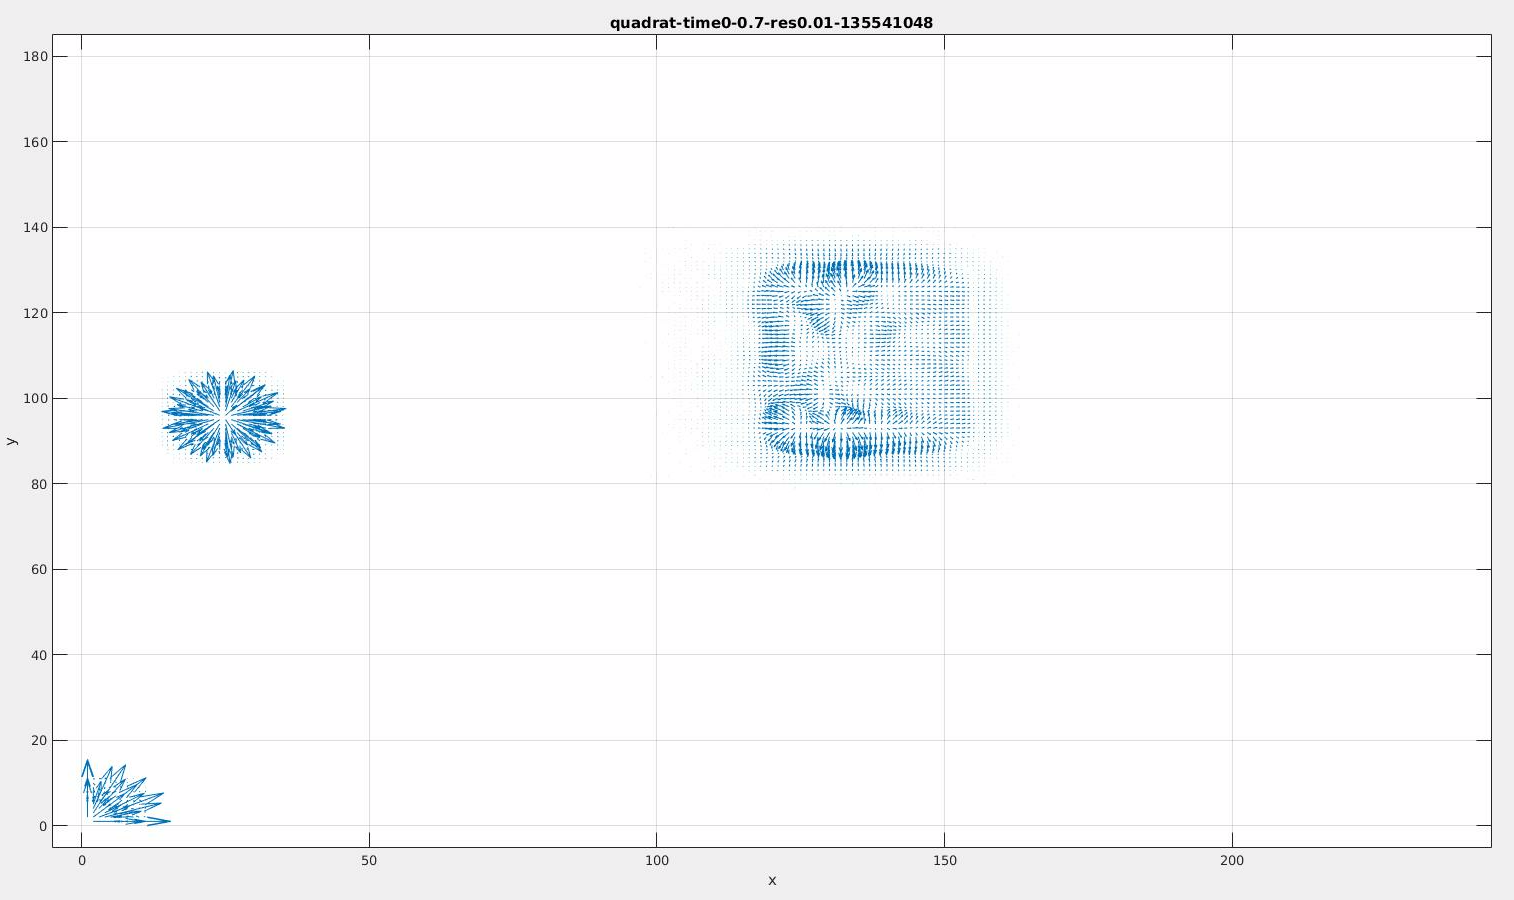
\includegraphics[height=.5\linewidth]{figs/defect-pixels/defect-quadrat.png}
  \caption{}
\end{subfigure}
\begin{subfigure}{.45\textwidth}
  \centering
  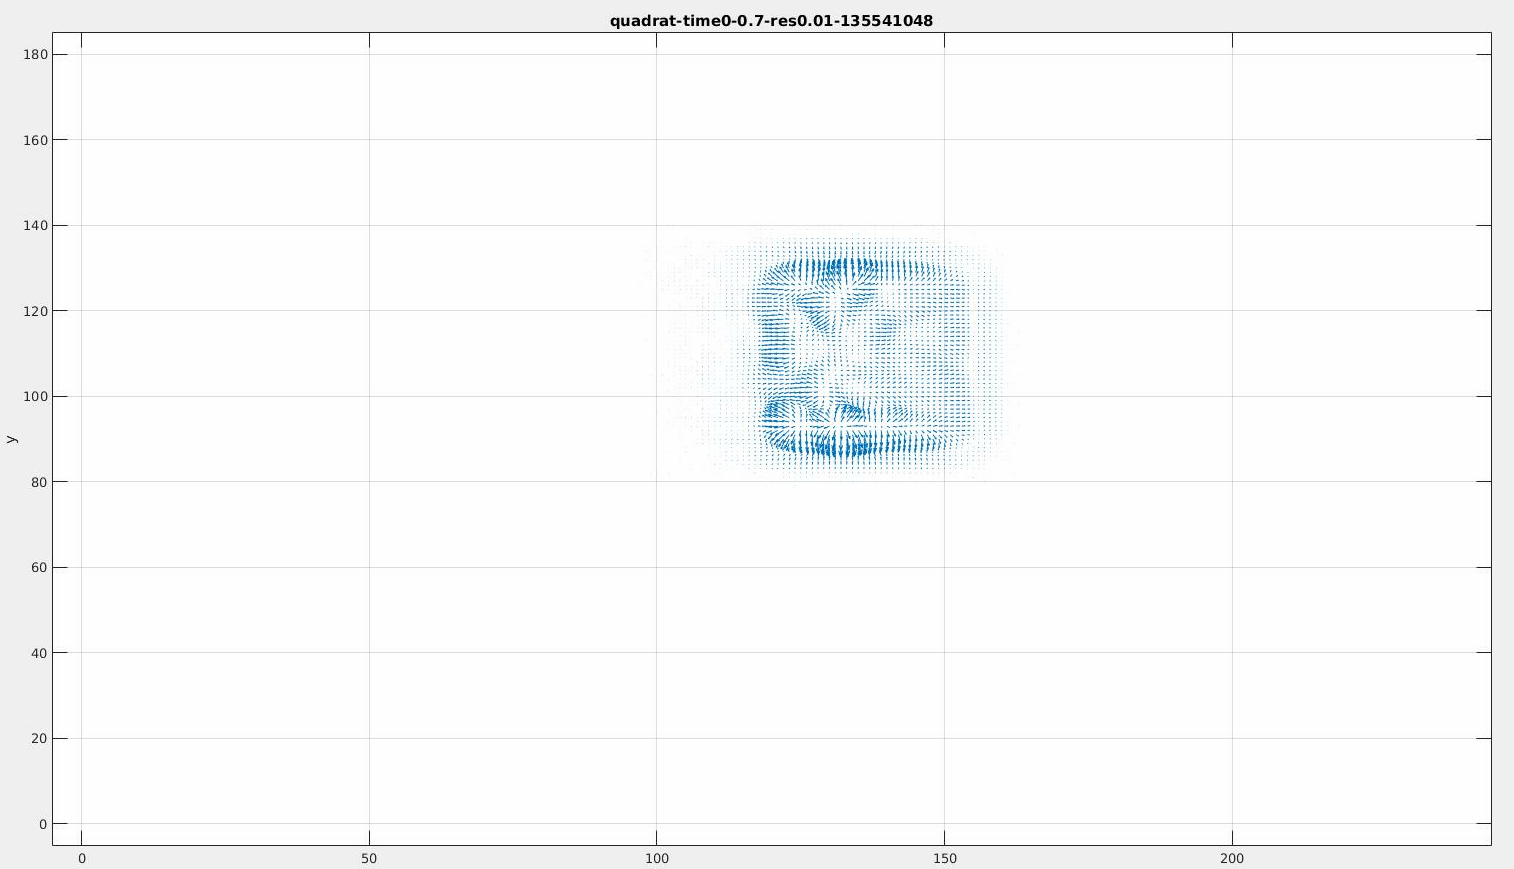
\includegraphics[height=.5\linewidth]{figs/defect-pixels/cleaned-quadrat.png}  \caption{}
\end{subfigure}
\caption[Preprocessing step: Removing events from defect pixels.]{Comparison of the flow before and after the defect pixel clean up. Image (a) shows high responses in the left and lower left corner, which are caused by defect pixels. Through manually feeding the coordinates into an event converter script, the defect events are removed from the data and artifacts are removed from the resulting flow field (b).}
\label{fig:defect-pixel-cleanup}
\end{figure}


To obtain more meaningful results, we manually eliminate these pixels from the event data.
To do so, the event data is firstly inspected in the jAER Viewer. 
Within the software, all recorded pixel coordinates can be analyzed individually.
With the \textit{Hot Pixels} filter, locations of pixels that are triggered very often within a certain time frame can be easily determined.
%Check whether florian mentions data formats
\edit{Given the locations of the defect pixels, a readout script for \textit{.aedat} files. }{ there's no verb; what's with the script?}
The script reads out the position, time and parity for all events and deletes all defect events.
The event data is then extended with a unique ID for each event and saved as a tabular file.
%This way, the event data is readable by the c++ program, which is used to read, write and convert event data.
% and decrements the index value for all following events.

%The event data is saved in a binary format.
%To further process the data, 

\paragraph{Evaluation}
\edit{A first,}{ was there A second?} thorough evaluation of a simple geometric scene was conducted.
This was done to ensure the correctness of the algorithm and test its performance for different parameter choices.
The scene consists of a horizontally moving rectaungular object (see Figure \ref{fig:quadrat-snapshots}).


In this experiment, we only inspect the locations of events of increasing intensity.
We do this, because we want to investigate the angular error in comparison to the ground truth in a meaningful way. 
At the \textit{off}-event locations, the event-based flow is pointing in opposite direction, which leads to a large offset of the average angular error. 
A close-up view that shows the described masking of the flow field is shown in Figure \ref{fig:qaudrat-close-masking}.


The ground truth provides a time stamp for each frame of the ground truth flow.
While the event data is quantized to Event Slices, a second set of time stamps is generated for each slice of events.
As the ground truth frames are not created for the exact same times as the quantized slices, we first have to determine the best fitting ground truth flow field for each slice.
For the evaluation, two different approaches of comparing the computed flow with the ground truth are applied.
Firstly, we directly compare each slice with the ground truth frame for which the difference of the two respective time stamps is smallest.
Secondly, we linearly interpolate from the two closest ground truth frames that have been recorded before and after the time of the event slice.


We observe that the flow directions at the corners of the vertical edge tend to point outwards instead of pointing in $x$-direction. 
This is likely caused by the aperture problem and could be tackled in future experiments by performing a normalization step in the preprocessing.
Table \ref{tab:error_comparison_square} shows a comparison of calculated errors for the moving square. The RMSE, mean, and median angular error between the computed flow and the ground truth are calculated. 
The median error dropped to below $5^\circ$ for some parameter settings without additional normalization. 


\begin{figure}[tb]
\centering
\begin{subfigure}{.45\textwidth}
  \centering
  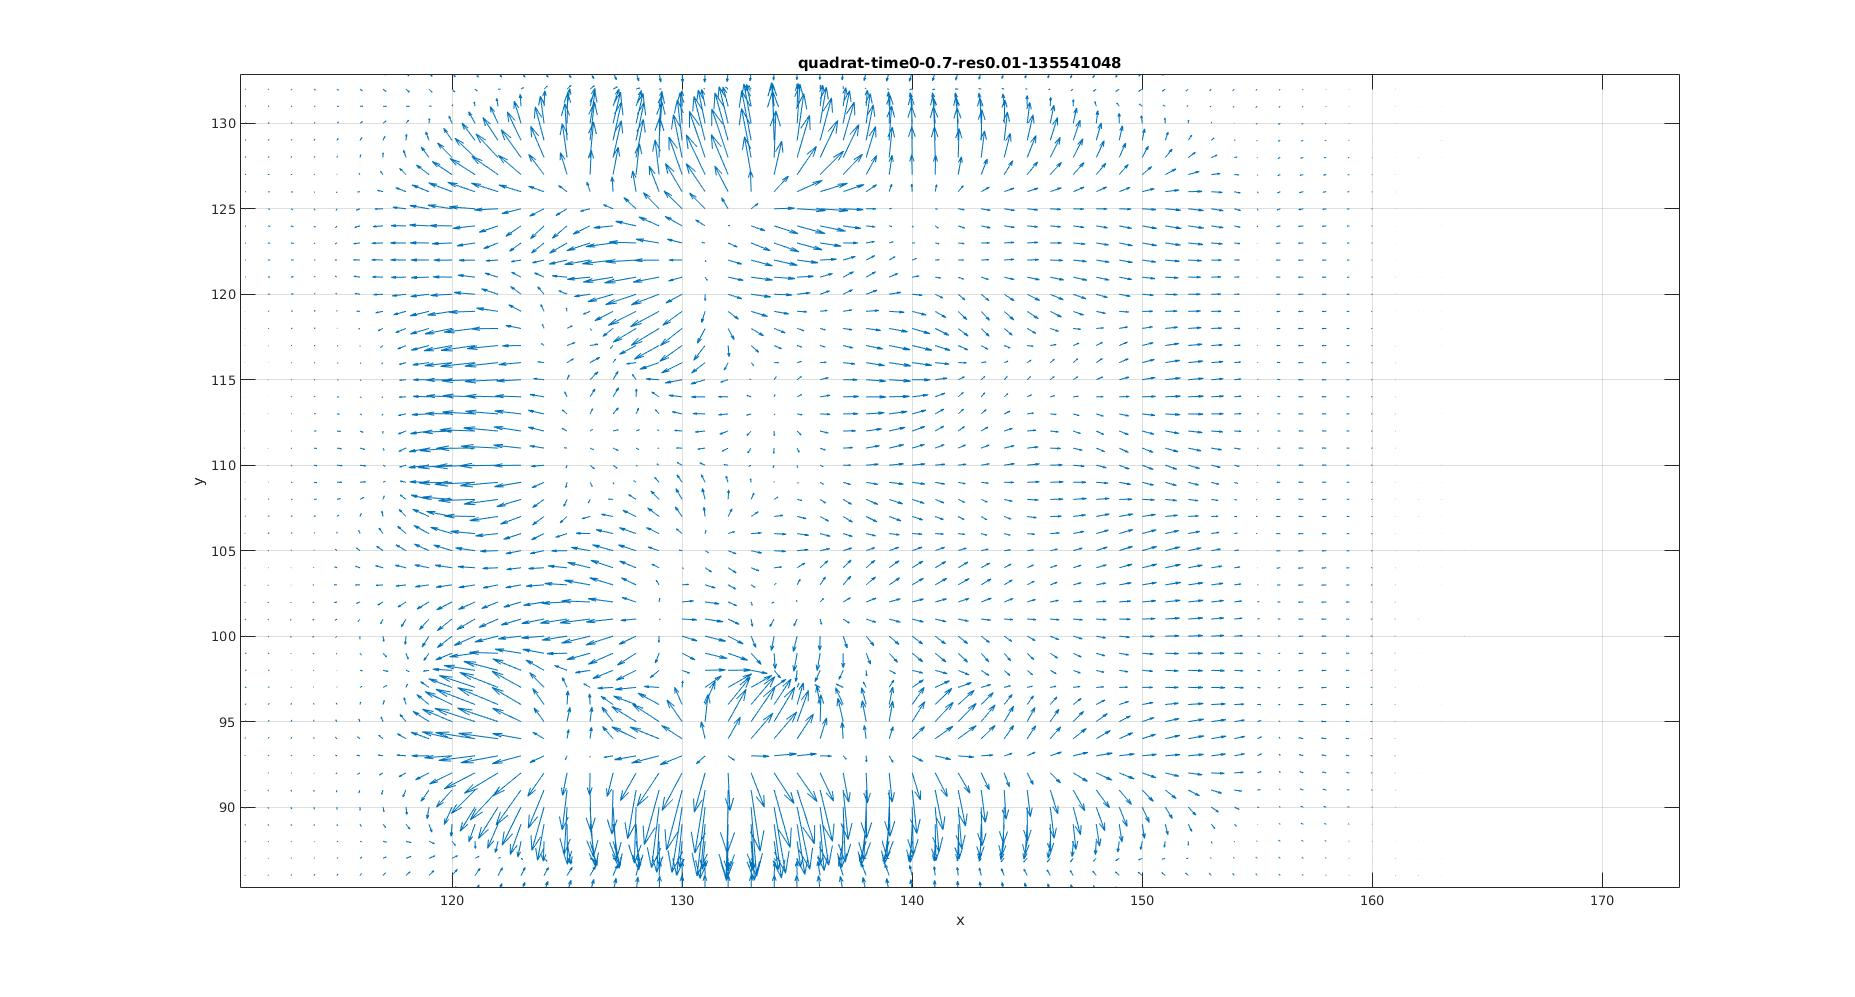
\includegraphics[height=.6\linewidth]{figs/quadrat_close.jpg}
  \caption{}
  \label{fig:qaudrat-close-masking-1}
\end{subfigure}
\begin{subfigure}{.45\textwidth}
  \centering
  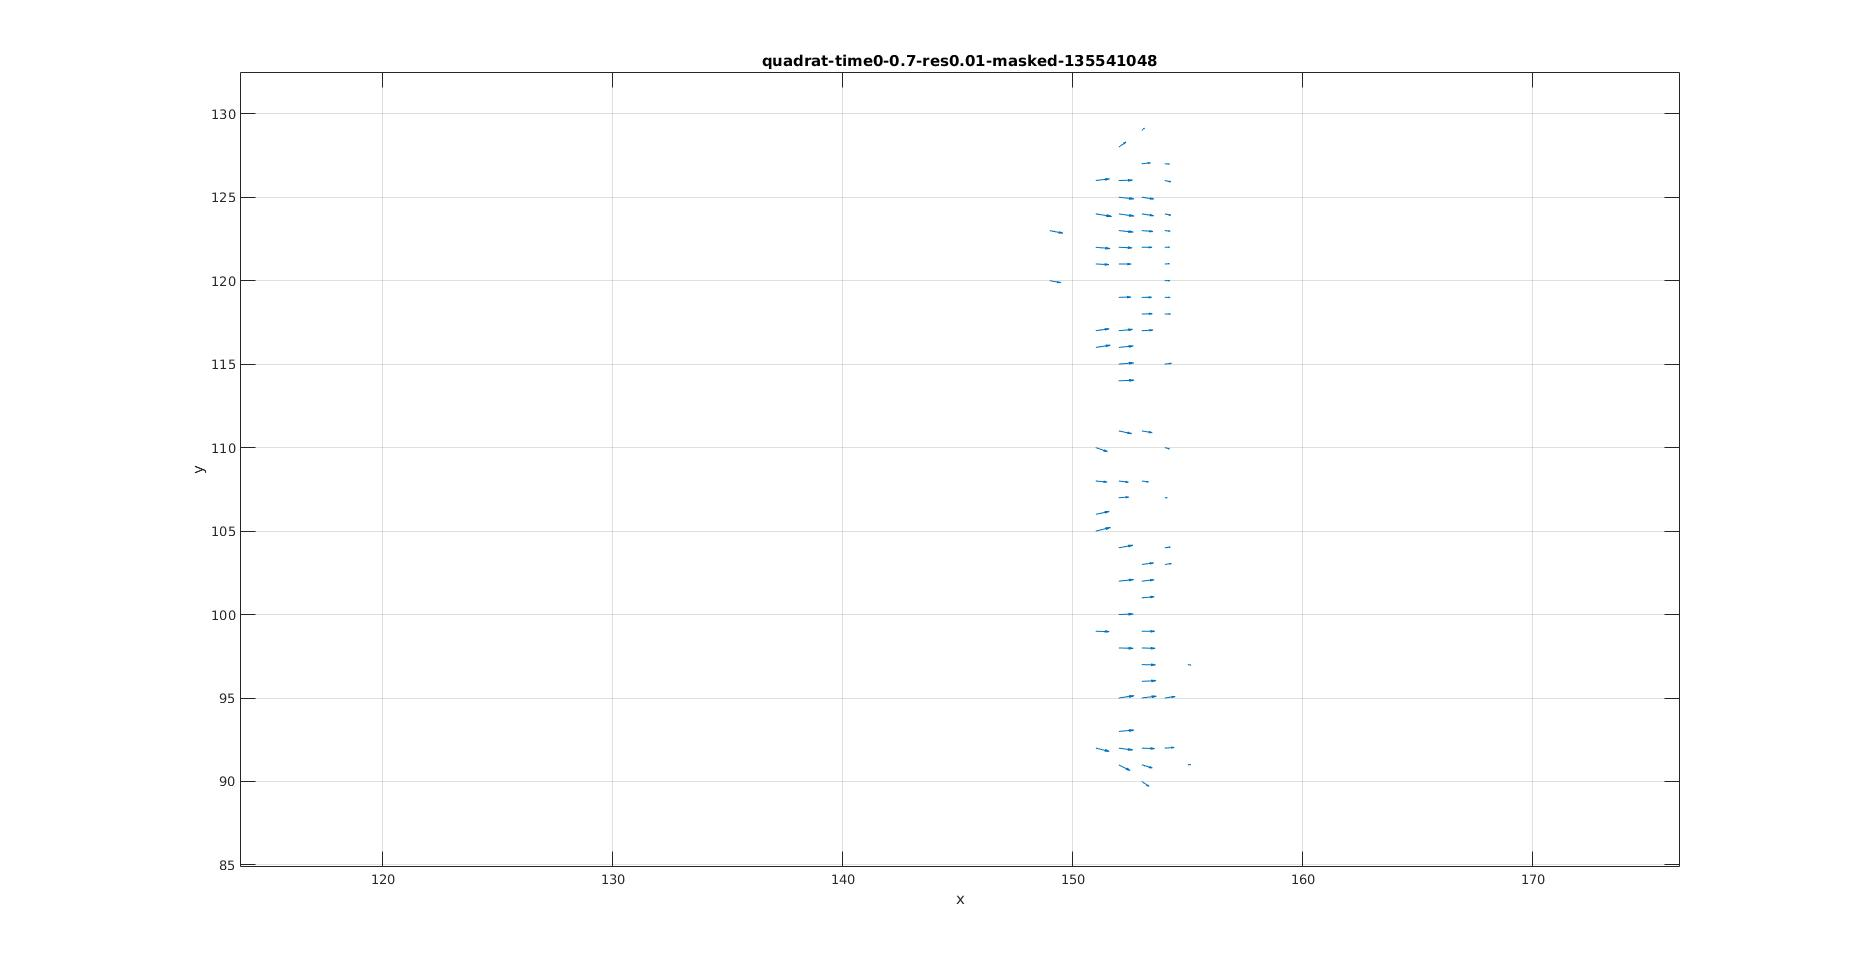
\includegraphics[height=.6\linewidth]{figs/quadrat_close_mask.jpg}
  \caption{}
  \label{fig:qaudrat-close-masking-2}
\end{subfigure}
\begin{subfigure}{.45\textwidth}
  \centering
  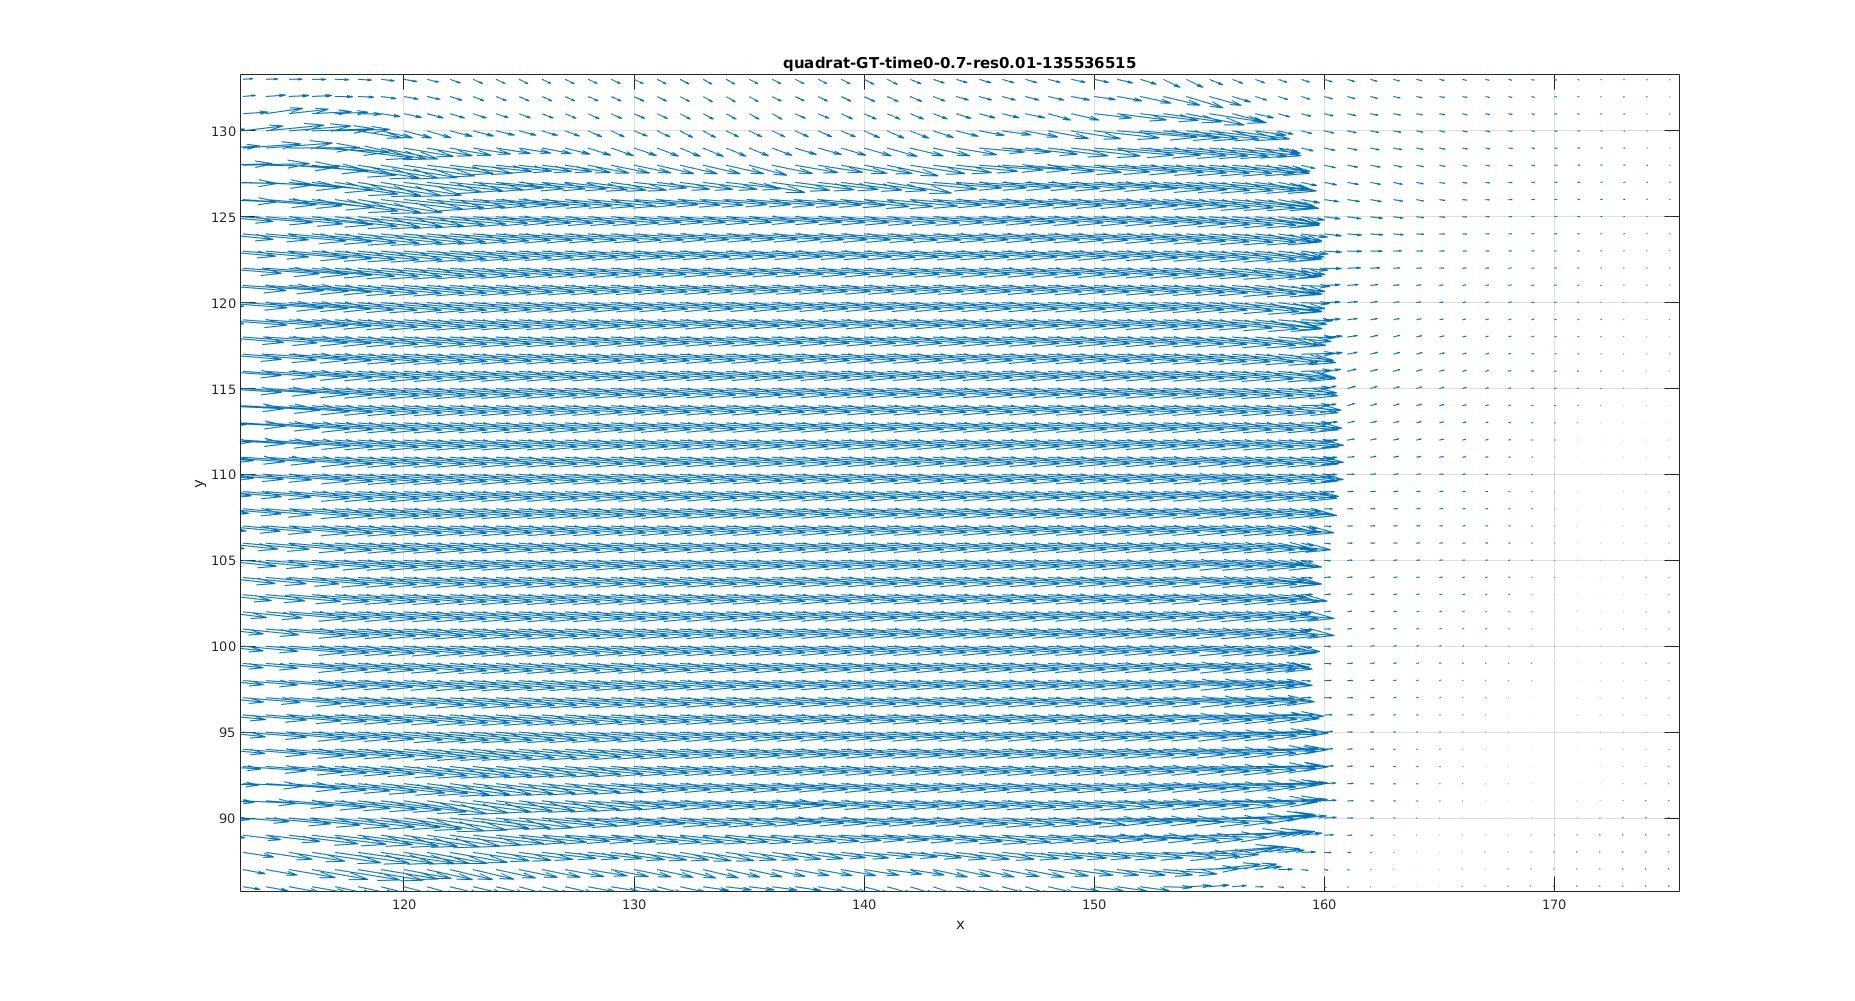
\includegraphics[height=.6\linewidth]{figs/quadrat_close_GT.jpg}
  \caption{}
  \label{fig:qaudrat-close-masking-3}
\end{subfigure}
\begin{subfigure}{.45\textwidth}
  \centering
  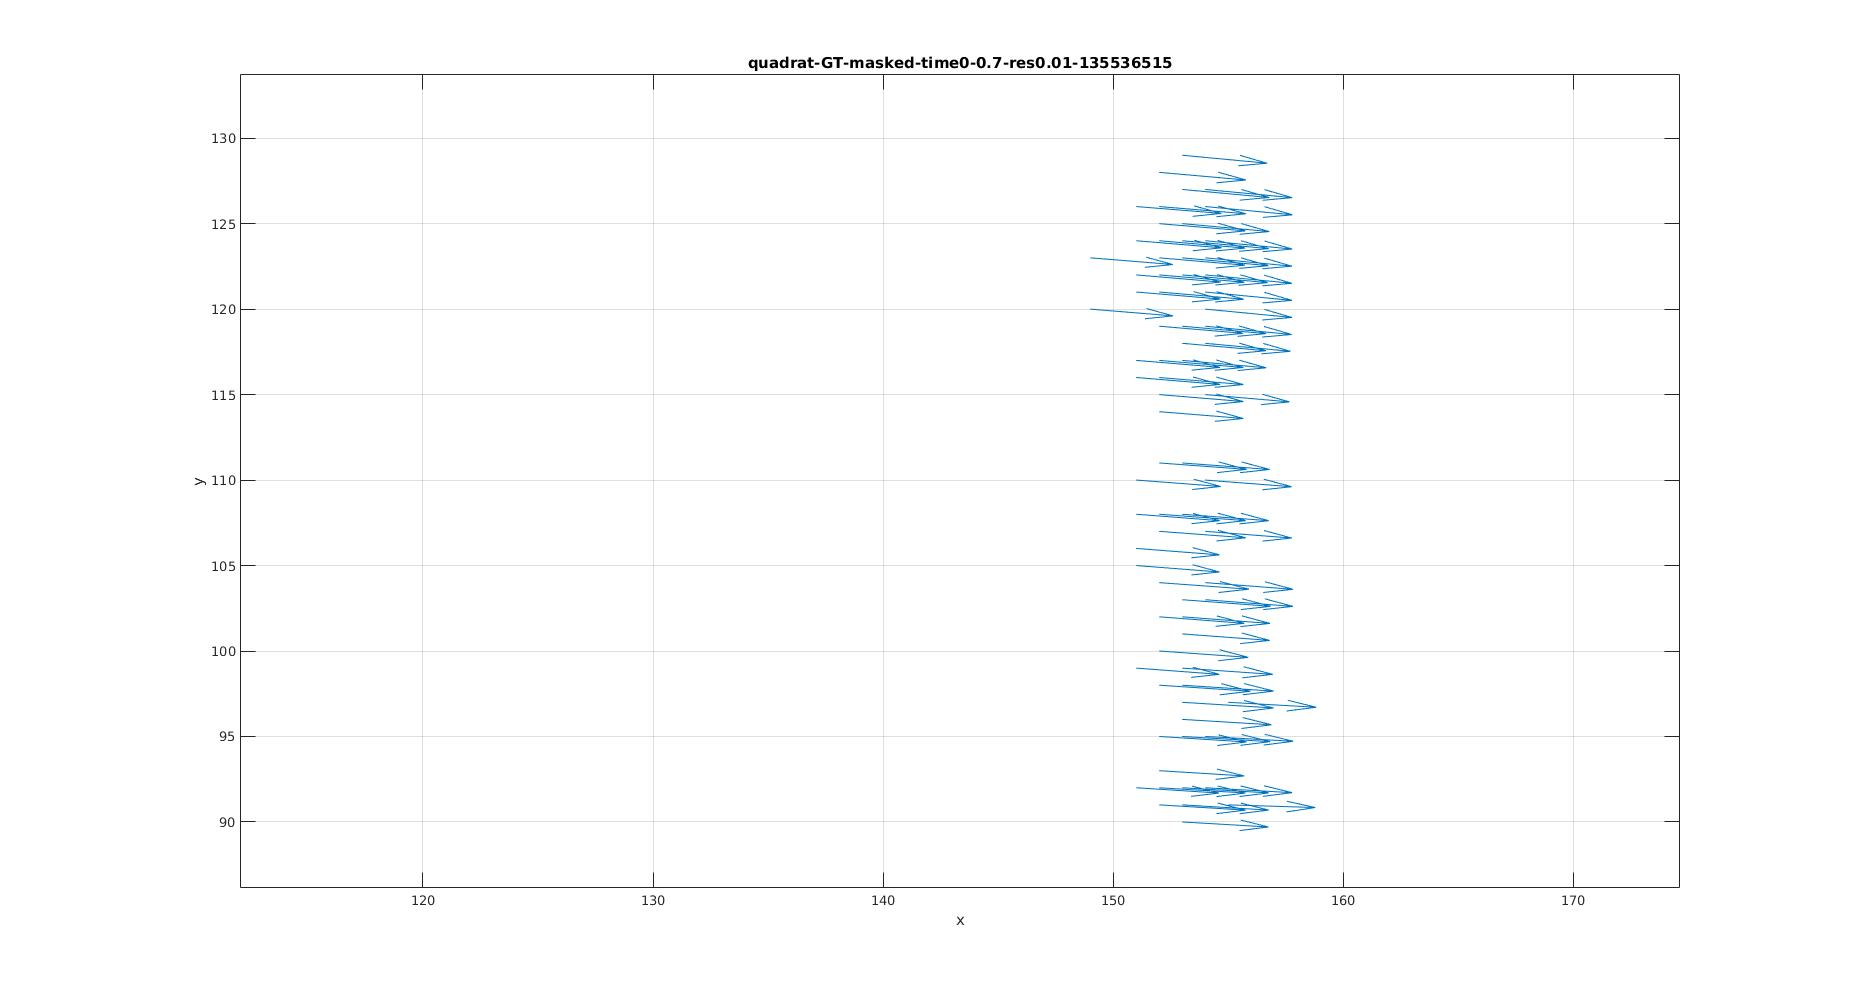
\includegraphics[height=.6\linewidth]{figs/quadrat_close_GT_masked.jpg}
  \caption{}
  \label{fig:qaudrat-close-masking-4}
\end{subfigure}
\caption[First scene: Square moving to the right.]{A moving square was recorded with the DVS sensor.
The flow field computed by the event-based optical flow algorithm is shown in (a).
The corresponding ground truth frame is shown in Figure (c).
To evaluate the optical flow, a mask with the event locations for the corresponding slice is applied to the flow fields.
Figures (b) and (d) show the flow at these locations for the computed flow and the ground truth.
Only the flow values at the event locations are considered in the evaluation.
The flow in the ground truth is consistently directed in $x$-direction, whereas the computed flow is pointing outwards at the outer edges. This aperture effect is likely compensable through normalization.}
\label{fig:qaudrat-close-masking}
\end{figure}

\begin{figure}[tb]
\centering
\begin{subfigure}{.45\textwidth}
  \centering
  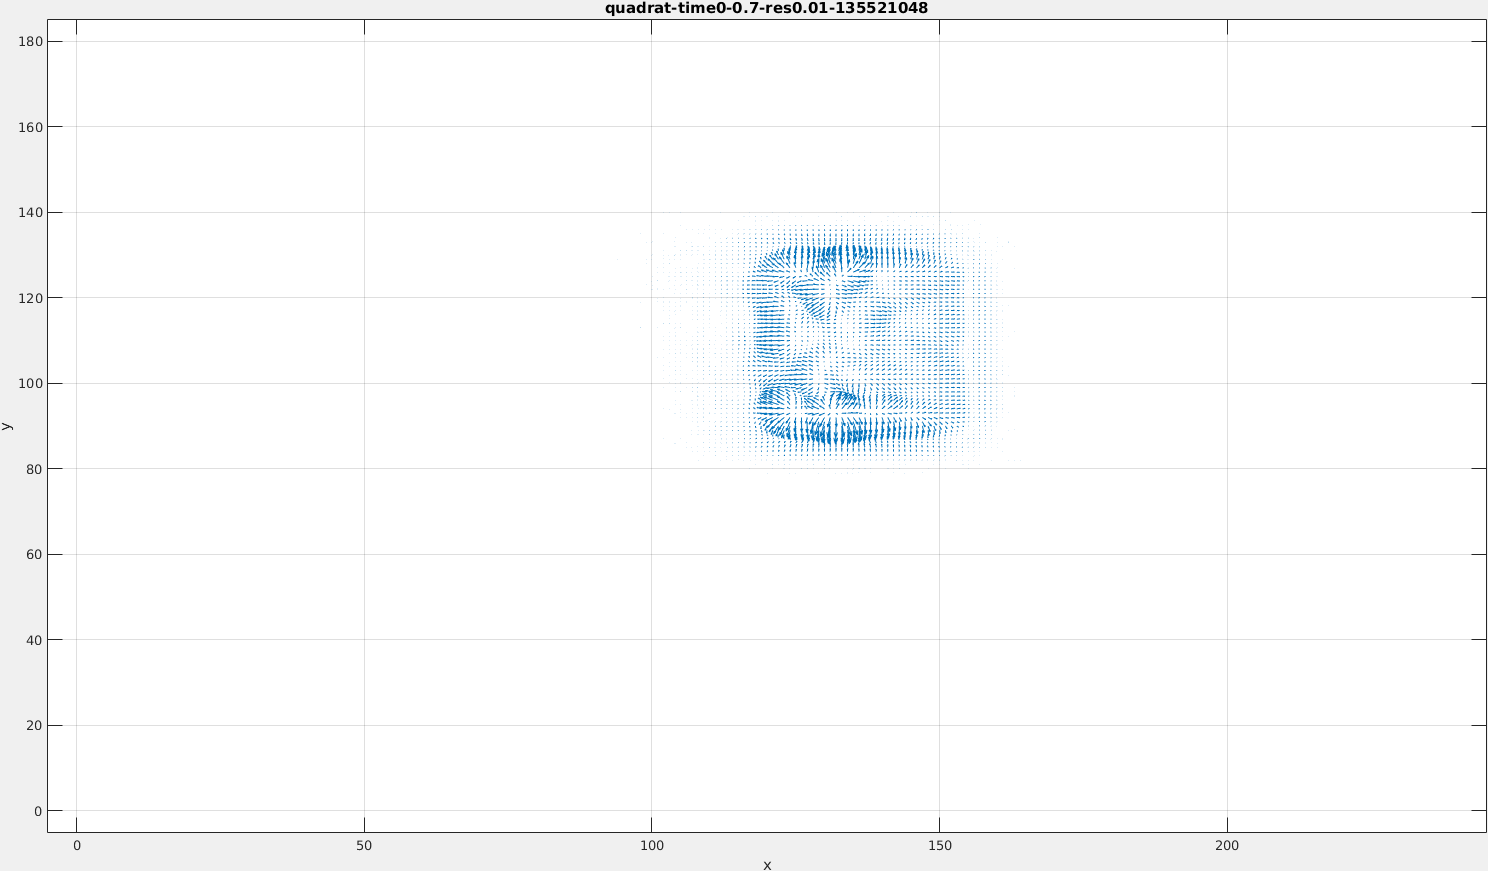
\includegraphics[height=.6\linewidth]{figs/quadrat/quadrat-1.png}
  \caption{}
\end{subfigure}
\begin{subfigure}{.45\textwidth}
  \centering
  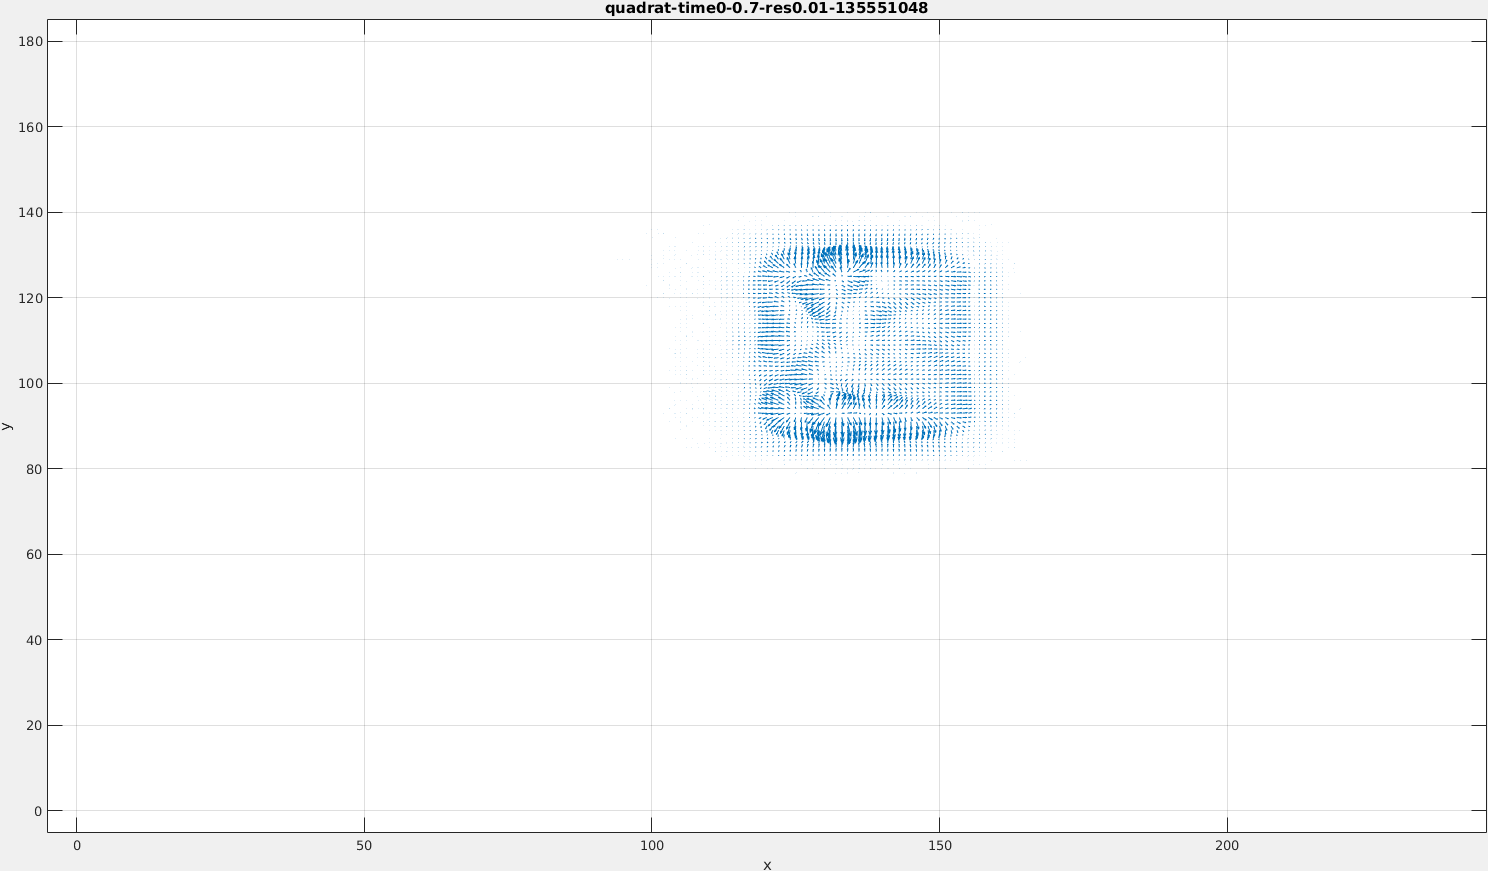
\includegraphics[height=.6\linewidth]{figs/quadrat/quadrat-2.png}
  \caption{}
\end{subfigure}
\begin{subfigure}{.45\textwidth}
  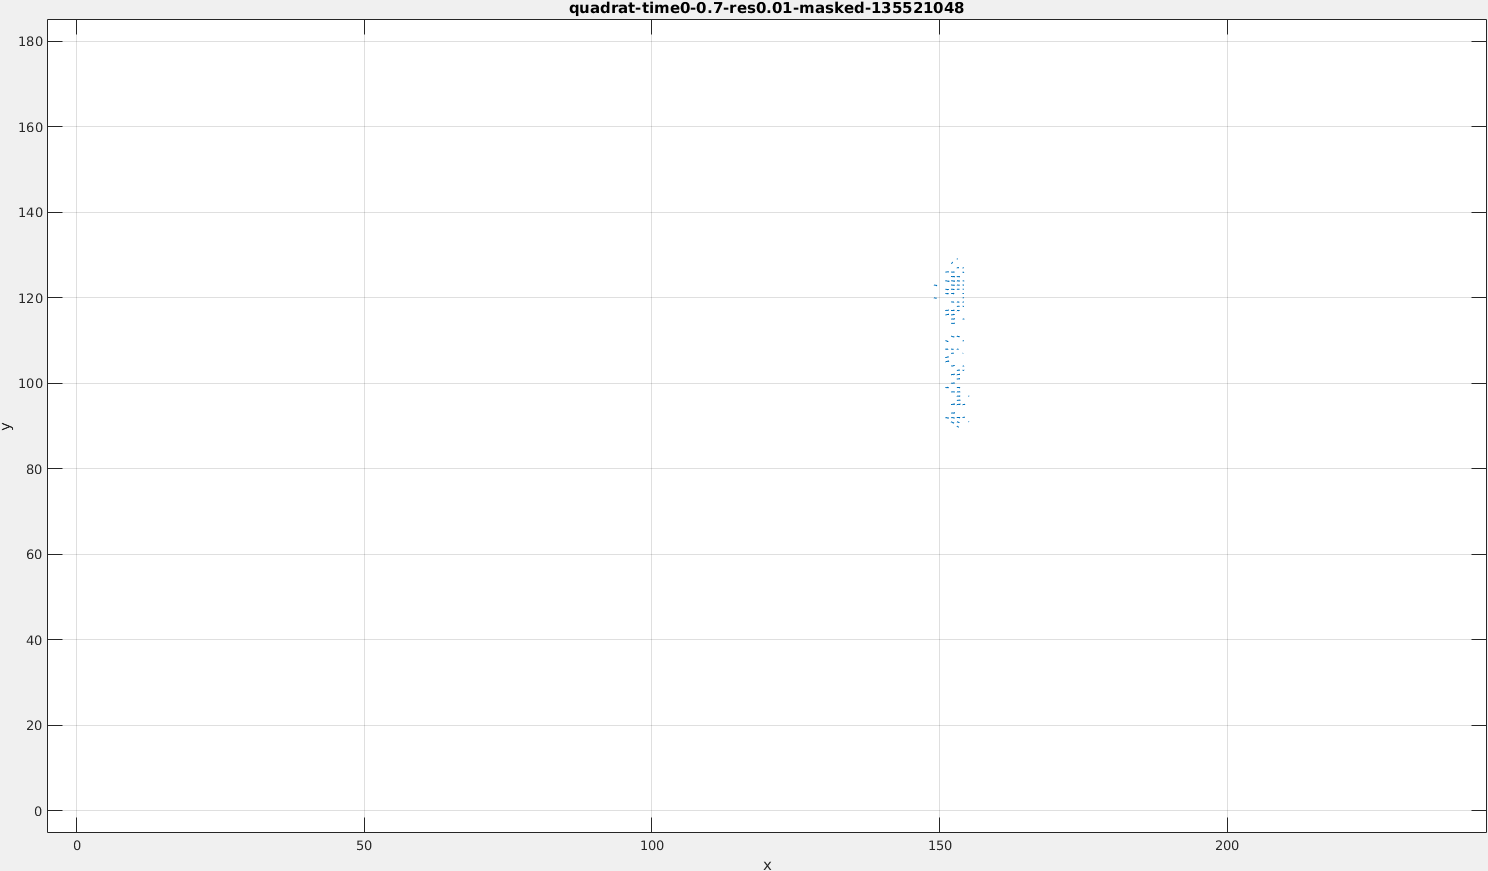
\includegraphics[height=.6\linewidth]{figs/quadrat/quadrat-masked-1.png}
  \caption{}
\end{subfigure}
\begin{subfigure}{.45\textwidth}
  \centering
  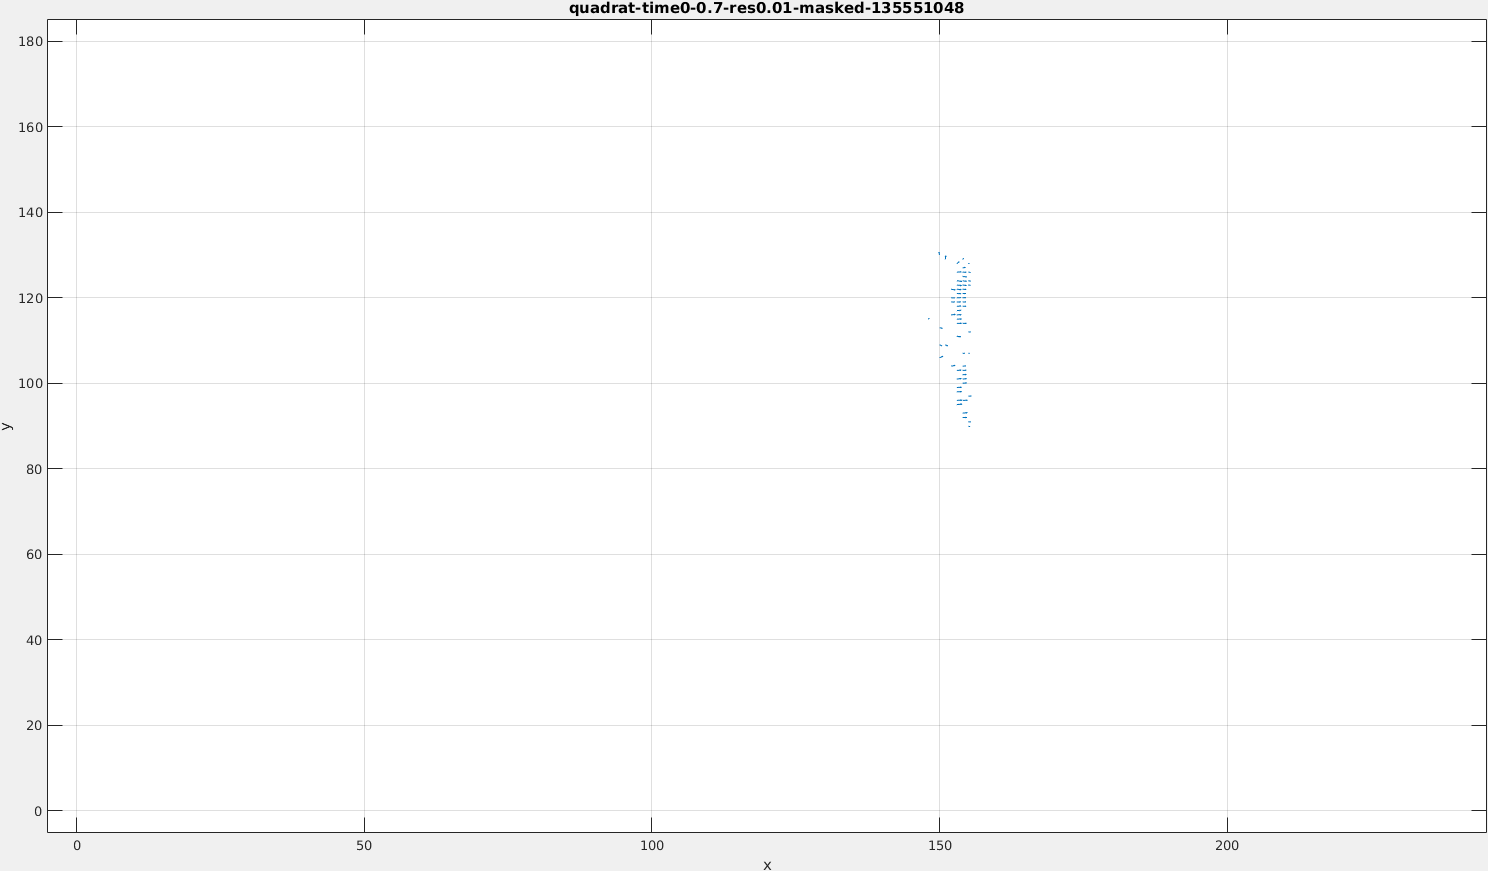
\includegraphics[height=.6\linewidth]{figs/quadrat/quadrat-masked-2.png}
  \caption{}
\end{subfigure}
\begin{subfigure}{.45\textwidth}
  \centering
  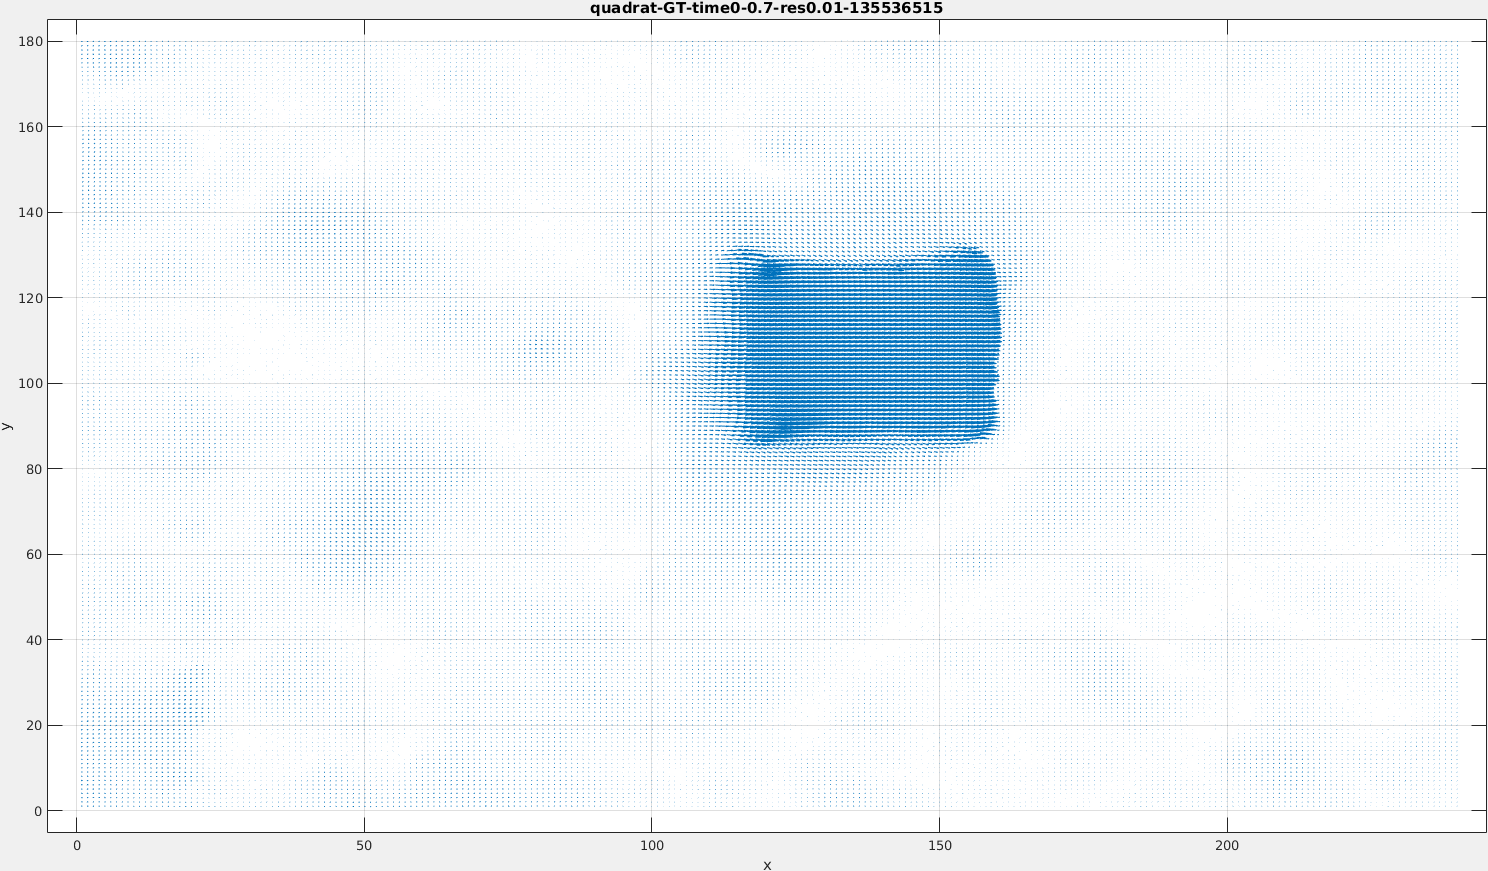
\includegraphics[height=.6\linewidth]{figs/quadrat/quadrat-GT-1.png}
  \caption{}
\end{subfigure}
\begin{subfigure}{.45\textwidth}
  \centering
  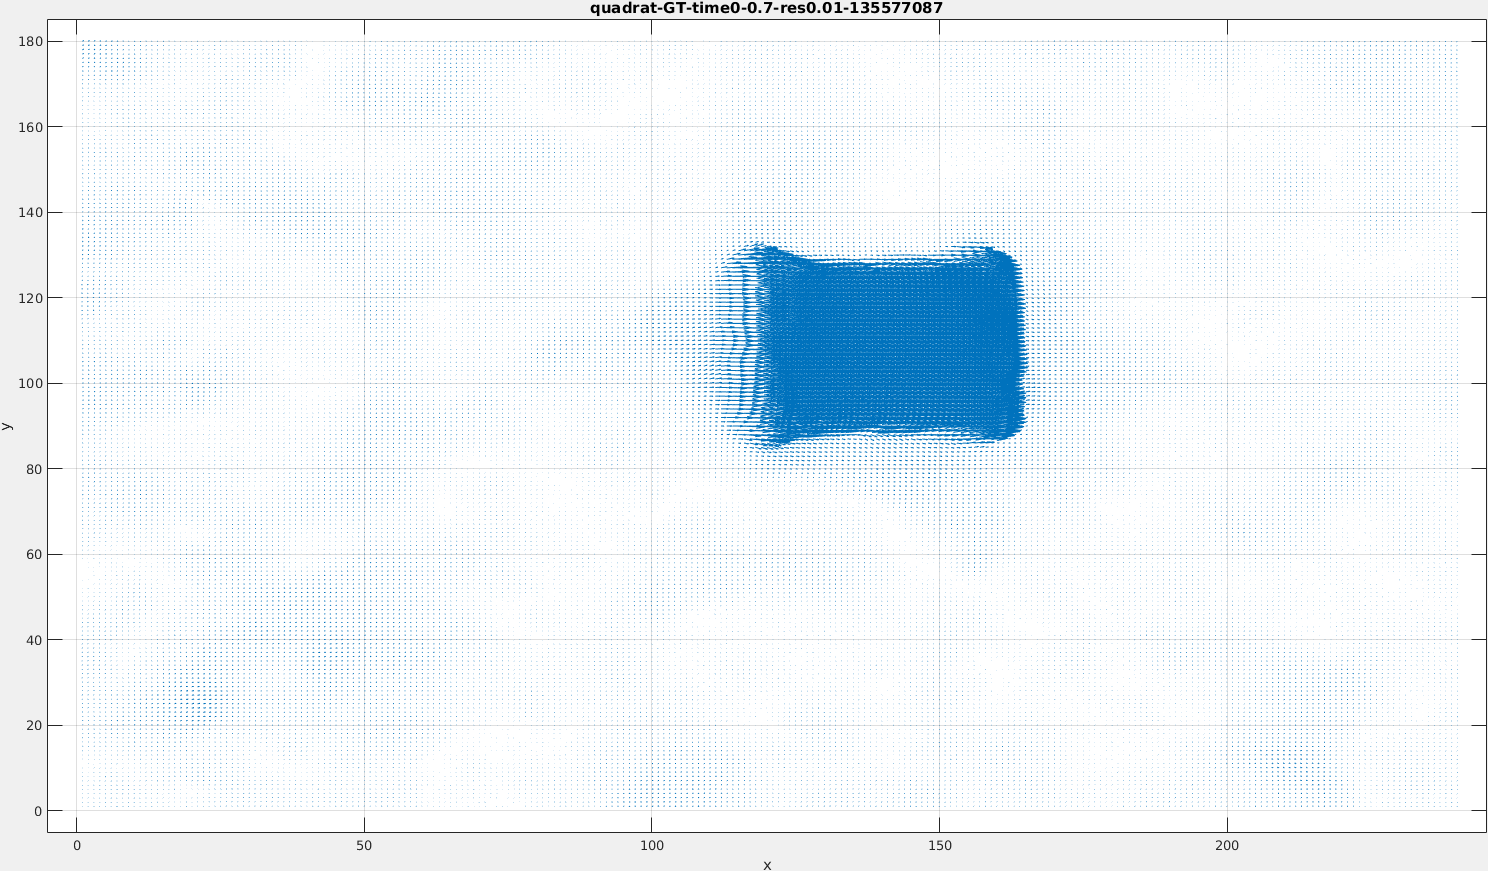
\includegraphics[height=.6\linewidth]{figs/quadrat/quadrat-GT-2.png}
  \caption{}
\end{subfigure}
\begin{subfigure}{.45\textwidth}
  \centering
  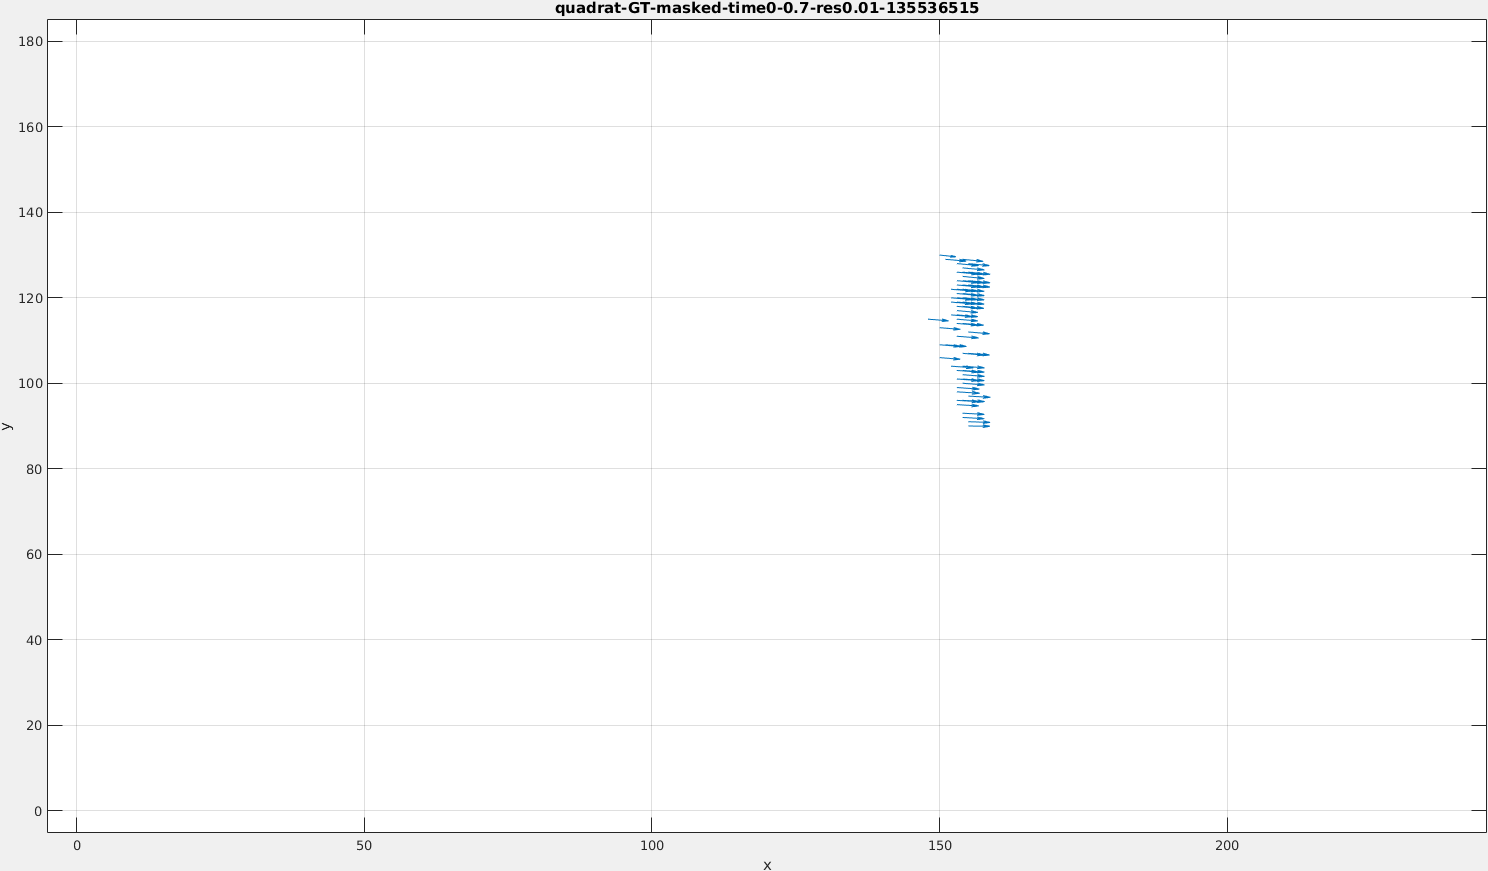
\includegraphics[height=.6\linewidth]{figs/quadrat/quadrat-GT-masked-1.png}
  \caption{}
\end{subfigure}
\begin{subfigure}{.45\textwidth}
  \centering
  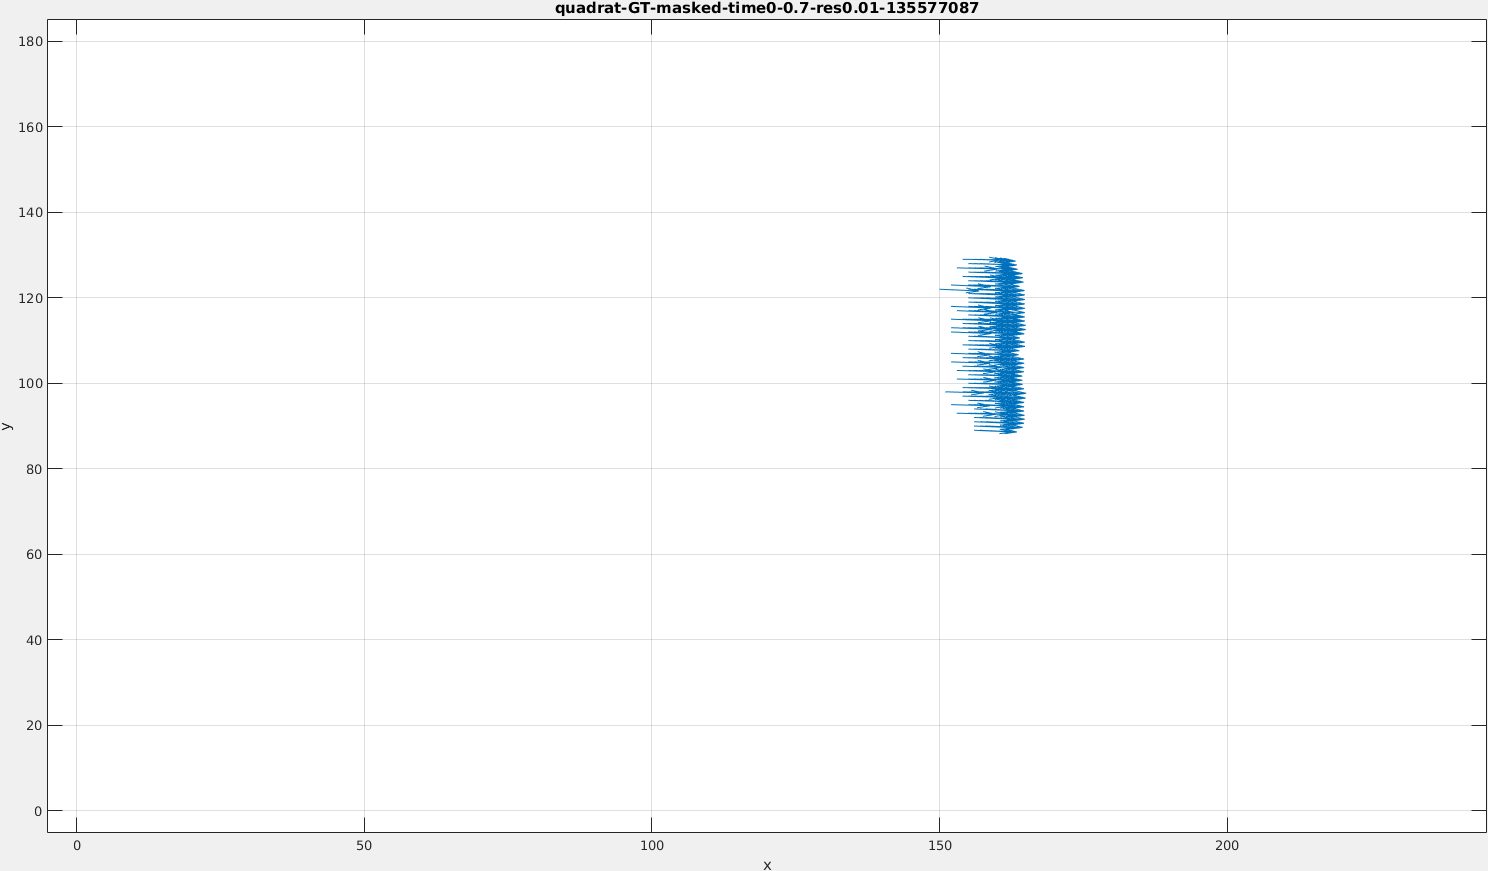
\includegraphics[height=.6\linewidth]{figs/quadrat/quadrat-GT-masked-2.png}
  \caption{}
\end{subfigure}
\caption[First scene: Robot approaching the DVS sensor.]{Second scene: Robot approaching the DVS sensor.
Figures (a) and (b) show the computed optical flow for the scene at two time steps. The masked flow fields are shown in Figures (c) and (d).
The corresponding ground truth is shown in Figures (e) and (f). Applying the same mask leads to Figures (g) and (h)}
\label{fig:quadrat-snapshots}
\end{figure}


\begin{table}[tb]
	\centering
		\begin{tabular}{lccccccc}
Scene & Setting & Matching & RMSE & MeanErr & MedianErr & Avg. Angle \\
\hline  \hline
quadrat & $1$ & direct & $33.70$ & $15.10$ & $5.13$ & $1.15$ & \\
quadrat & $1$ & interp & $33.79$ & $15.26$ & $5.09$ &  & \\
quadrat & $2$ & direct & $33.48$ & $15.04$ & $5.20$ & $1.23$ & \\
quadrat & $2$ & interp & $33.57$ & $15.21$ & $5.16$ &  & \\
quadrat & $3$ & direct & $22.41$ & $11.04$ & $4.89$ & $1.12$ & \\
quadrat & $3$ & interp & $22.48$ & $11.14$ & $4.91$ &  & \\
quadrat & $4$ & direct & $21.84$ & $10.85$ & $4.96$ & $1.16$ & \\
quadrat & $4$ & interp & $21.82$ & $10.96$ & $4.97$ &  & \\
quadrat & $5$ & direct & $19.58$ & $11.66$ & $6.19$ & $1.29$ & \\
quadrat & $5$ & interp & $20.93$ & $12.61$ & $6.53$ &  & \\
quadrat & $6$ & direct & $19.21$ & $11.36$ & $6.19$ & $1.31$ & \\
quadrat & $6$ & interp & $20.69$ & $12.45$ & $6.75$ &  & \\
quadrat & $7$ & direct & $32.76$ & $15.46$ & $5.37$ & $1.18$ & \\
quadrat & $7$ & interp & $33.19$ & $15.75$ & $5.35$ &  & \\
quadrat & $8$ & direct & $32.53$ & $15.39$ & $5.43$ & $1.29$ & \\
quadrat & $8$ & interp & $32.96$ & $15.68$ & $5.43$ &  & \\
quadrat & $9$ & direct & $21.84$ & $11.14$ & $4.92$ & $1.12$ & \\
quadrat & $9$ & interp & $22.55$ & $11.44$ & $4.92$ &  & \\
quadrat & $10$ & direct & $21.60$ & $11.03$ & $4.93$ & $1.17$ & \\
quadrat & $10$ & interp & $22.32$ & $11.36$ & $4.97$ &  & \\
quadrat & $11$ & direct & $16.33$ & $10.38$ & $6.24$ & $1.21$ & \\
quadrat & $11$ & interp & $17.12$ & $10.81$ & $6.48$ &  & \\
quadrat & $12$ & direct & $15.99$ & $10.17$ & $6.26$ & $1.26$ & \\
quadrat & $12$ & interp & $16.86$ & $10.72$ & $6.62$ &  & \\
		\end{tabular}
	\caption[First scene: Comparison of angular errors for different parameters.]{Comparison of angular errors for the moving square scene.
	The Setting attribute describes the composition of the temporal filter length as well as temporal resolution.
	 These settings can be compared in table \ref{tab:parameter_settings}. Considering the provided ground truth, parameter combination 3 lead to the lowest median error. When considering the underlying scene with vertical edges moving in $x$-direction, the average angle in setting 5 points to even better results.}
	\label{tab:error_comparison_square}
\end{table}

\begin{table}[tb]
	\centering
		\begin{tabular}{lccc}
Setting & Filter Length [ms] & Temp. Res. [ms] & Angle incr. ($0$ to $360^\circ$) \\
\hline  \hline
$1$ & $0.30$ & $0.010$ & $45.00$\\
$2$ & $0.30$ & $0.010$ & $30.00$\\
$3$ & $0.50$ & $0.010$ & $45.00$\\
$4$ & $0.50$ & $0.010$ & $30.00$\\
$5$ & $0.70$ & $0.010$ & $45.00$\\
$6$ & $0.70$ & $0.010$ & $30.00$\\
$7$ & $0.30$ & $0.005$ & $45.00$\\
$8$ & $0.30$ & $0.005$ & $30.00$\\
$9$ & $0.50$ & $0.005$ & $45.00$\\
$10$ & $0.50$ & $0.005$ & $30.00$\\
$11$ & $0.70$ & $0.005$ & $45.00$\\
$12$ & $0.70$ & $0.005$ & $30.00$\\
$13$ & $0.20$ & $0.005$ & $45.00$\\
$14$ & $0.20$ & $0.005$ & $30.00$\\
$15$ & $0.03$ & $0.001$ & $45.00$\\
$16$ & $0.03$ & $0.001$ & $30.00$\\
		\end{tabular}
	\caption[Different parameter settings for the evaluations]{Different parameter settings have been used for the evaluation of the flow.
	 The spatial size of the filter remained constant during the experiments.
	 The filter length was adjusted as well as the temporal resolution, i.e. the distance between time slices. 
	 Furthermore, the composition of the filter bank was varied by changing the rotation of the individual Gabor filters. 
	 For this, Gabor filters were rotated by angles between $0$ and $360$ degrees with constant angular increments.}
	\label{tab:parameter_settings}
\end{table}


In the second scene, a small robot is approaching the DVS sensor.
In the ground truth we can observe that the average angle of the computed flow is about $-135^\circ$ (see Figure \ref{fig:pushbot-snapshots}). 
As seen in Table \ref{tab:error_comparison_pushbot}, angular error between the event-based optical flow and the ground truth is rather high in this case.
One reason for this is the movement direction of the robot.
In contrast to the first scene, the robot does not move in any direction perpendicular to its edges.
Without additional normalization the computed optical flow points only in the directions perpendicular to the edges, which is why the actual movement direction is not reflected properly by the computed flow.
Furthermore, noise and other contours on the surface of the robot cause flow in random directions to be detected.
This further increases the calculated angular error.
The average angle of the computed flow amounts to about $-100^\circ$, which is close to average angle of the ground truth flow, considering the missing normalization.


\begin{figure}[tb]
\centering
\begin{subfigure}{.45\textwidth}
  \centering
  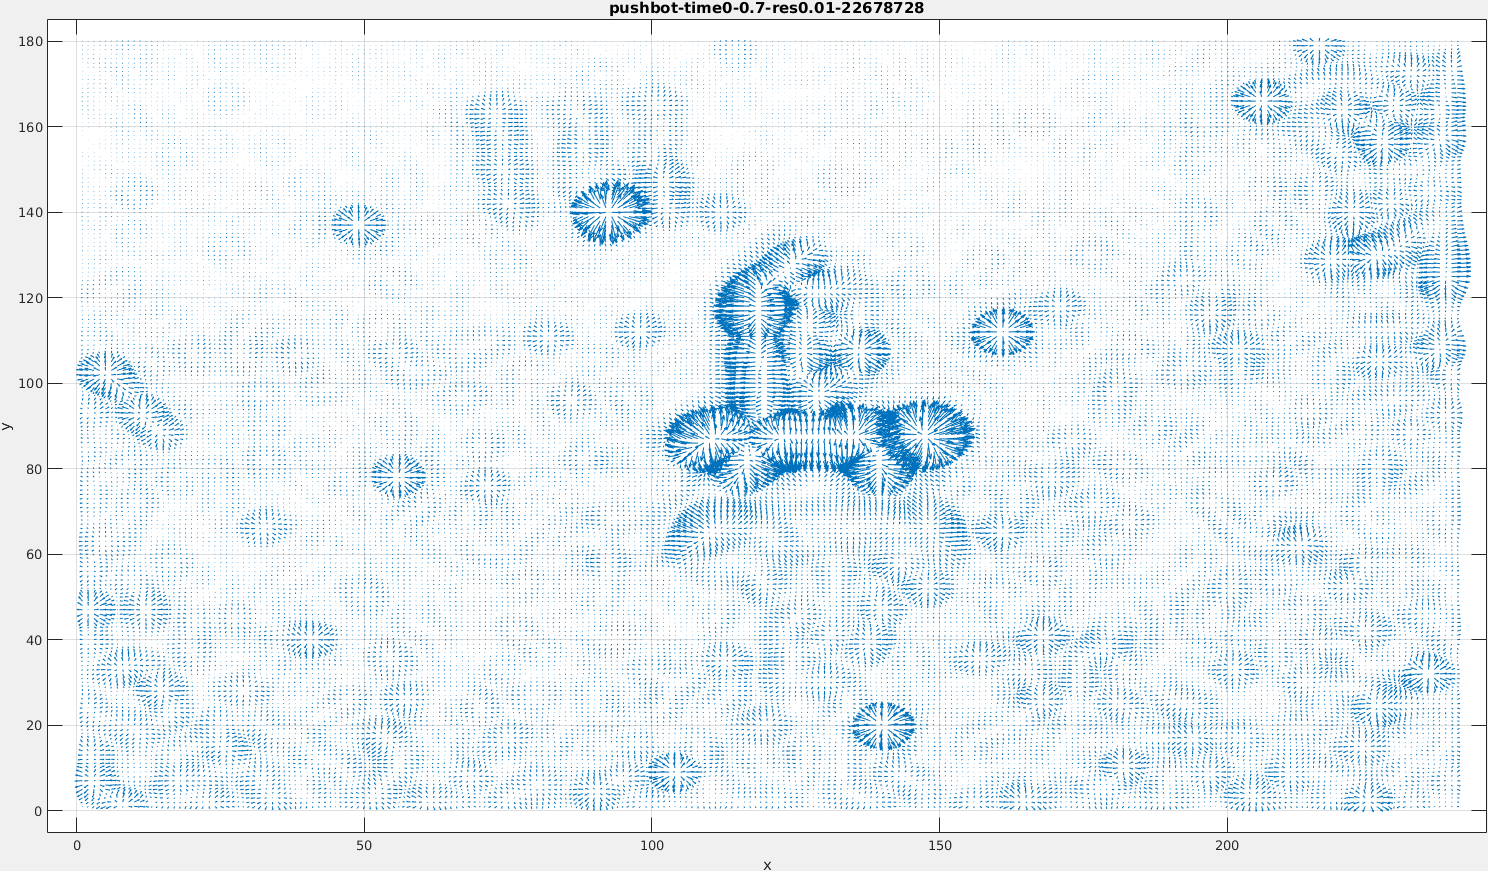
\includegraphics[height=.6\linewidth]{figs/pushbot/pushbot-1.png}
  \caption{}
\end{subfigure}
\begin{subfigure}{.45\textwidth}
  \centering
  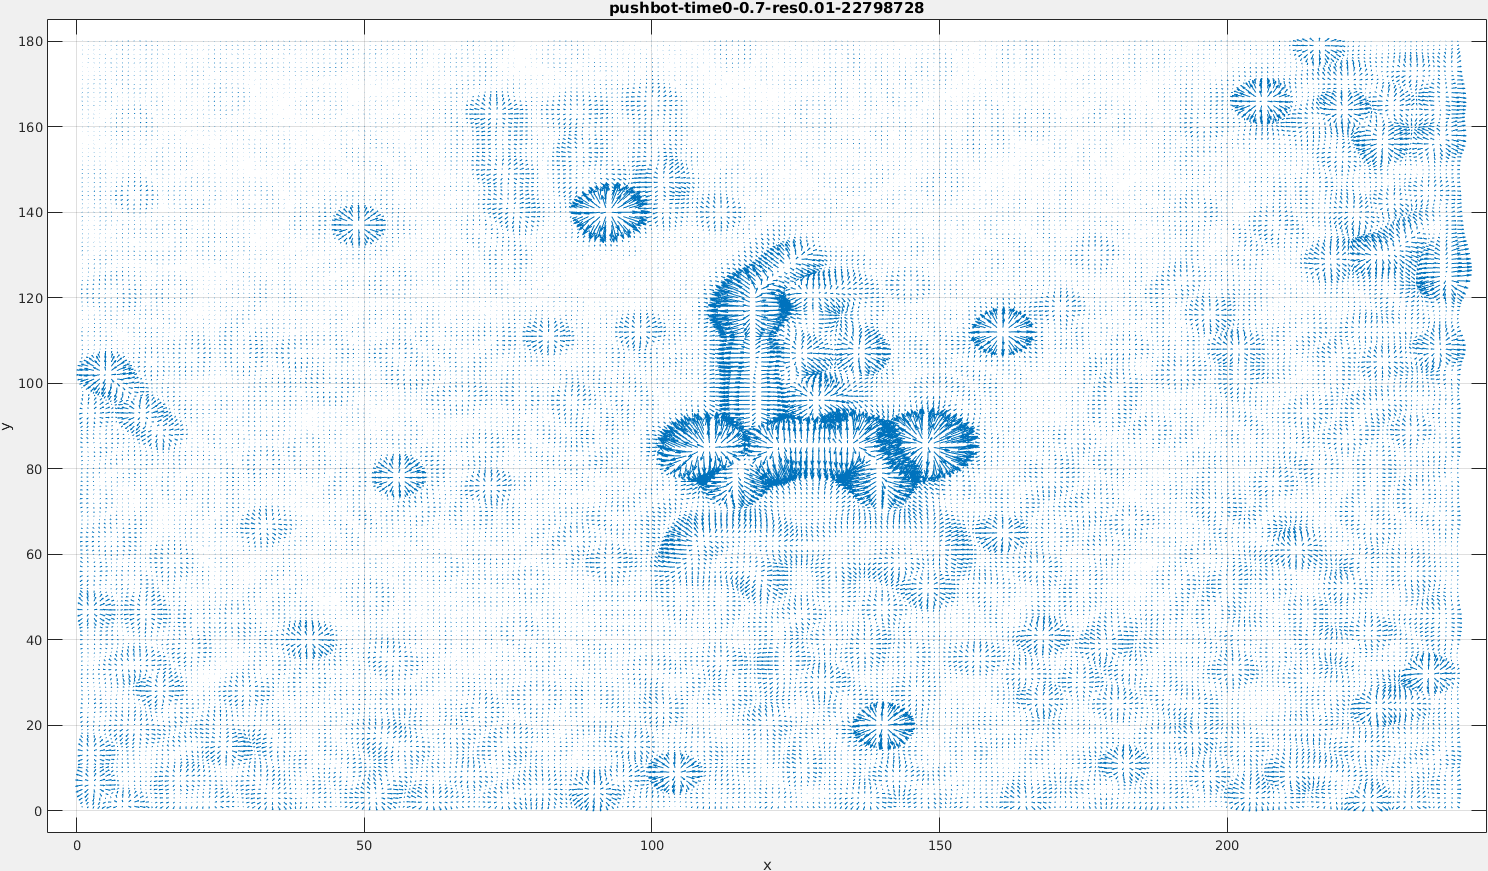
\includegraphics[height=.6\linewidth]{figs/pushbot/pushbot-2.png}
  \caption{}
\end{subfigure}
\begin{subfigure}{.45\textwidth}
  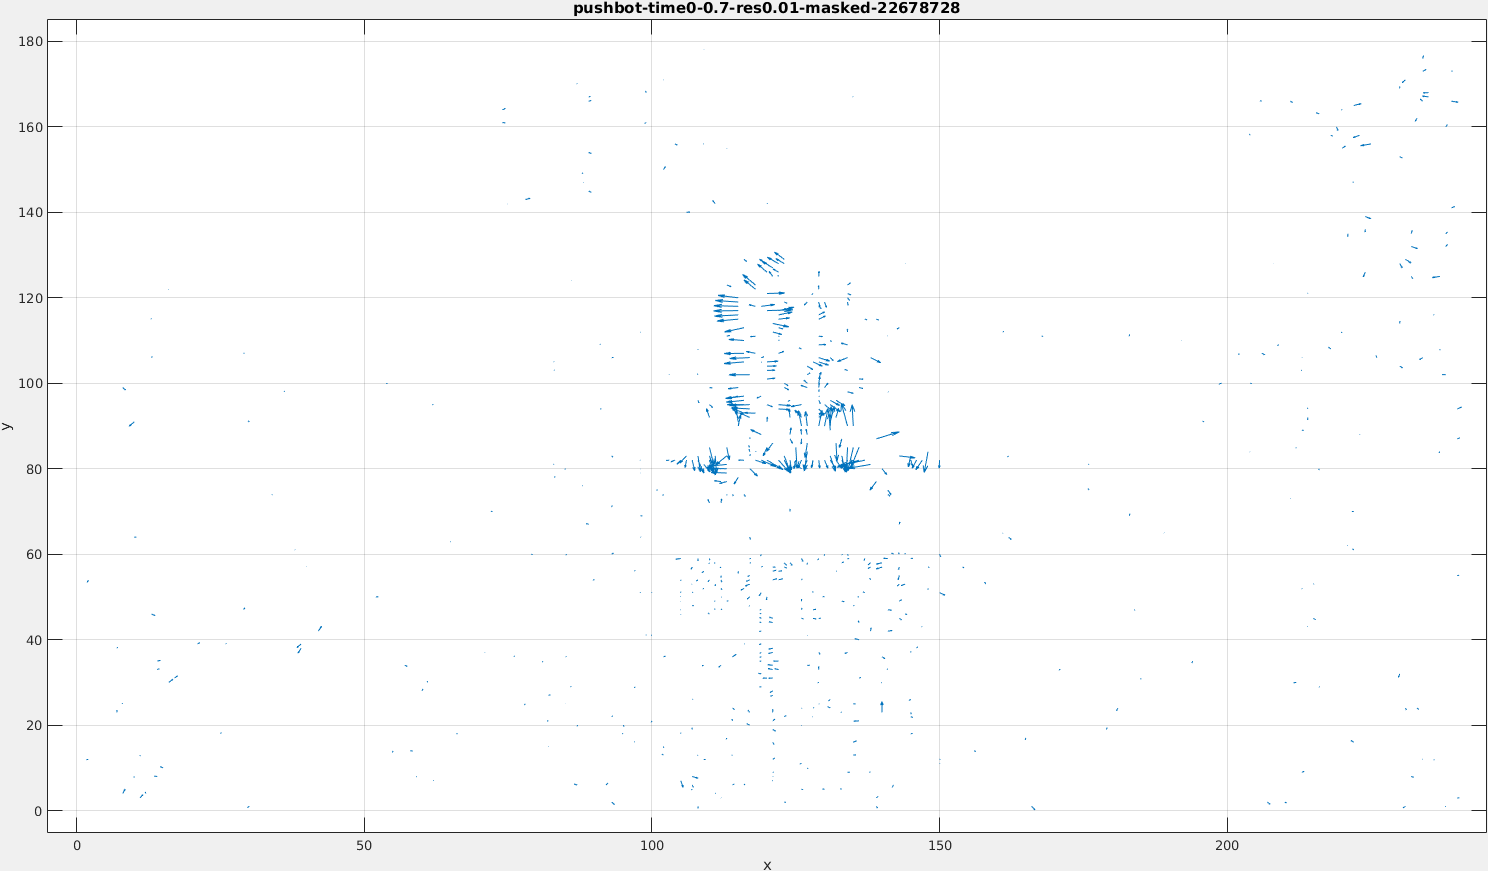
\includegraphics[height=.6\linewidth]{figs/pushbot/pushbot-masked-1.png}
  \caption{}
\end{subfigure}
\begin{subfigure}{.45\textwidth}
  \centering
  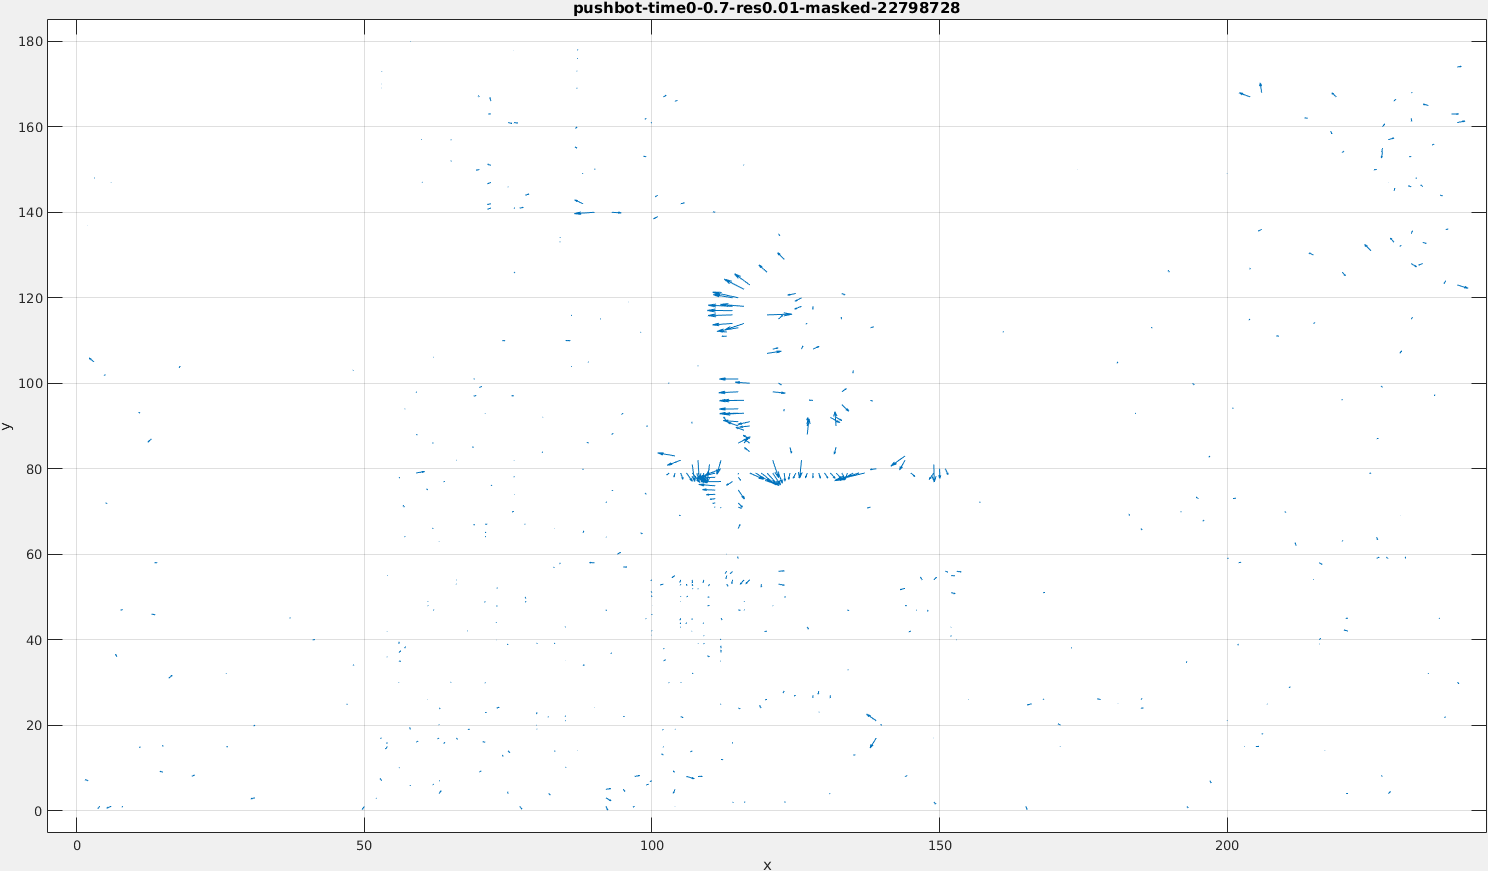
\includegraphics[height=.6\linewidth]{figs/pushbot/pushbot-masked-2.png}
  \caption{}
\end{subfigure}
\begin{subfigure}{.45\textwidth}
  \centering
  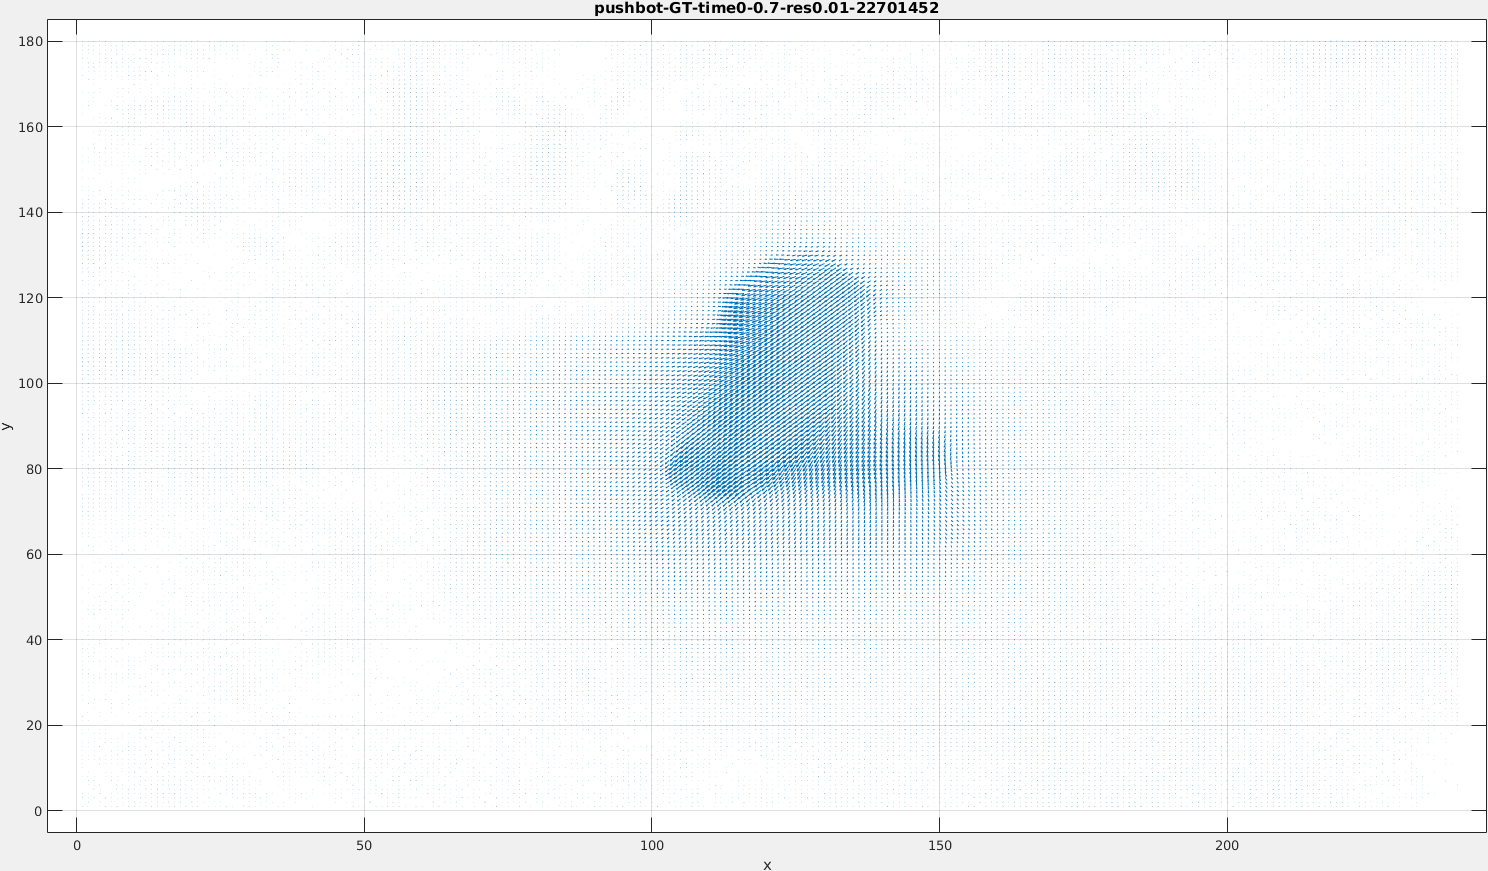
\includegraphics[height=.6\linewidth]{figs/pushbot/pushbot-GT-1.png}
  \caption{}
\end{subfigure}
\begin{subfigure}{.45\textwidth}
  \centering
  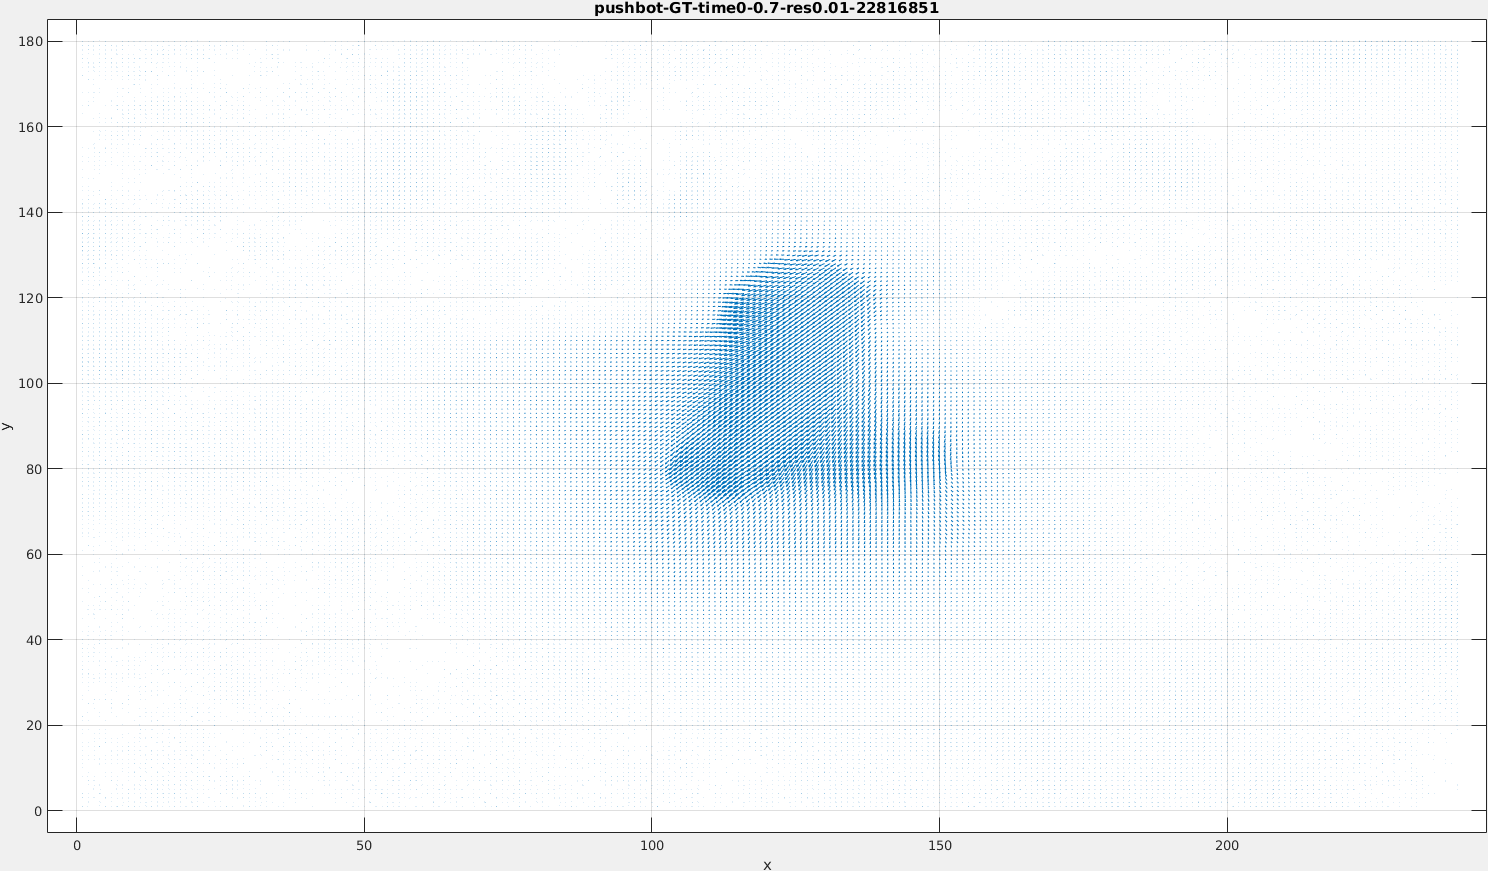
\includegraphics[height=.6\linewidth]{figs/pushbot/pushbot-GT-2.png}
  \caption{}
\end{subfigure}
\begin{subfigure}{.45\textwidth}
  \centering
  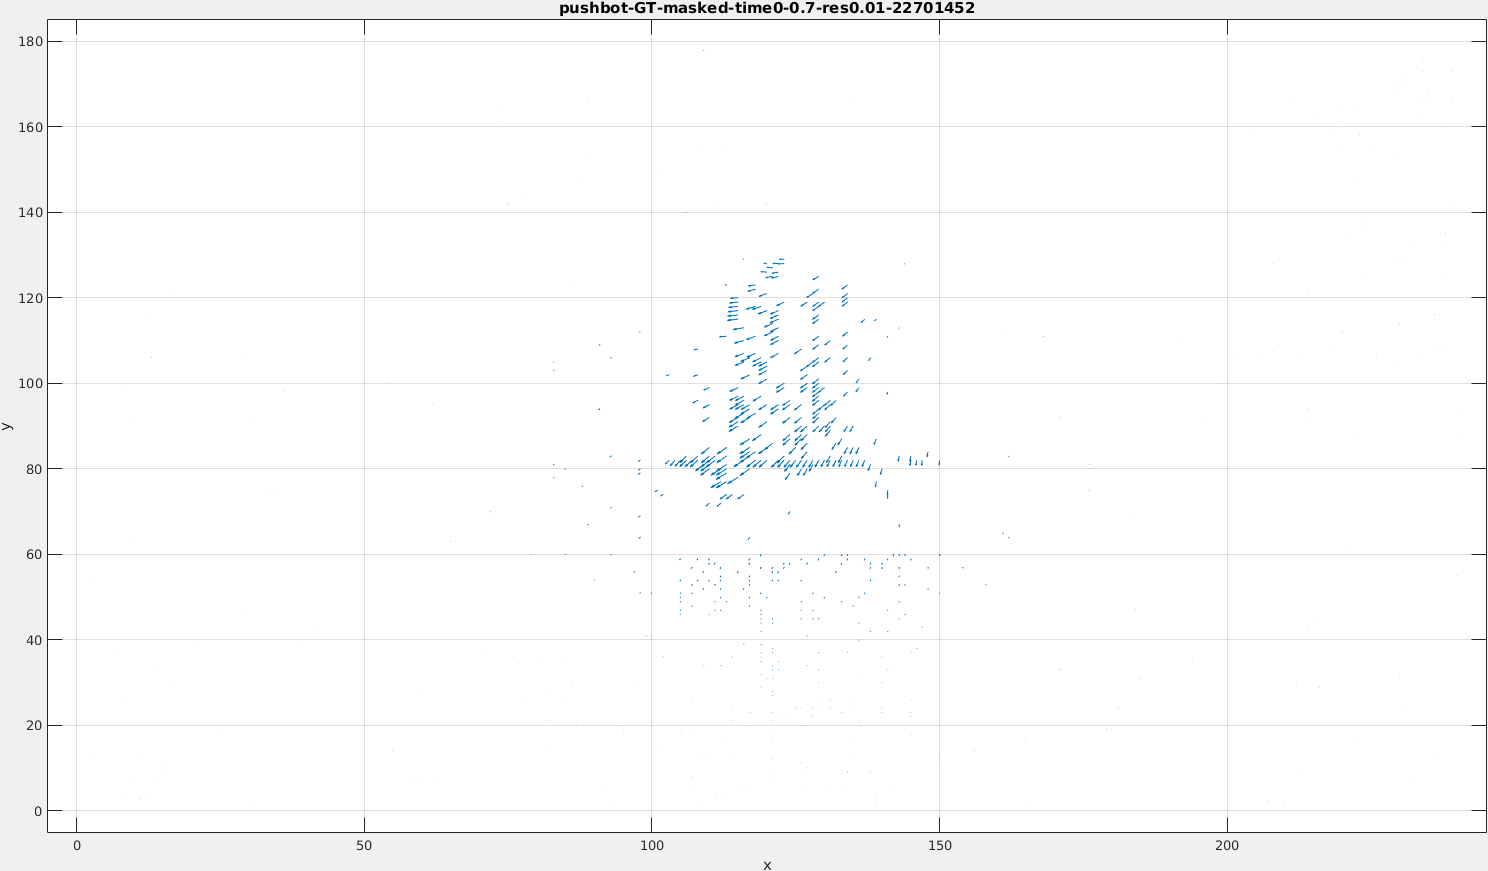
\includegraphics[height=.6\linewidth]{figs/pushbot/pushbot-GT-masked-1.png}
  \caption{}
\end{subfigure}
\begin{subfigure}{.45\textwidth}
  \centering
  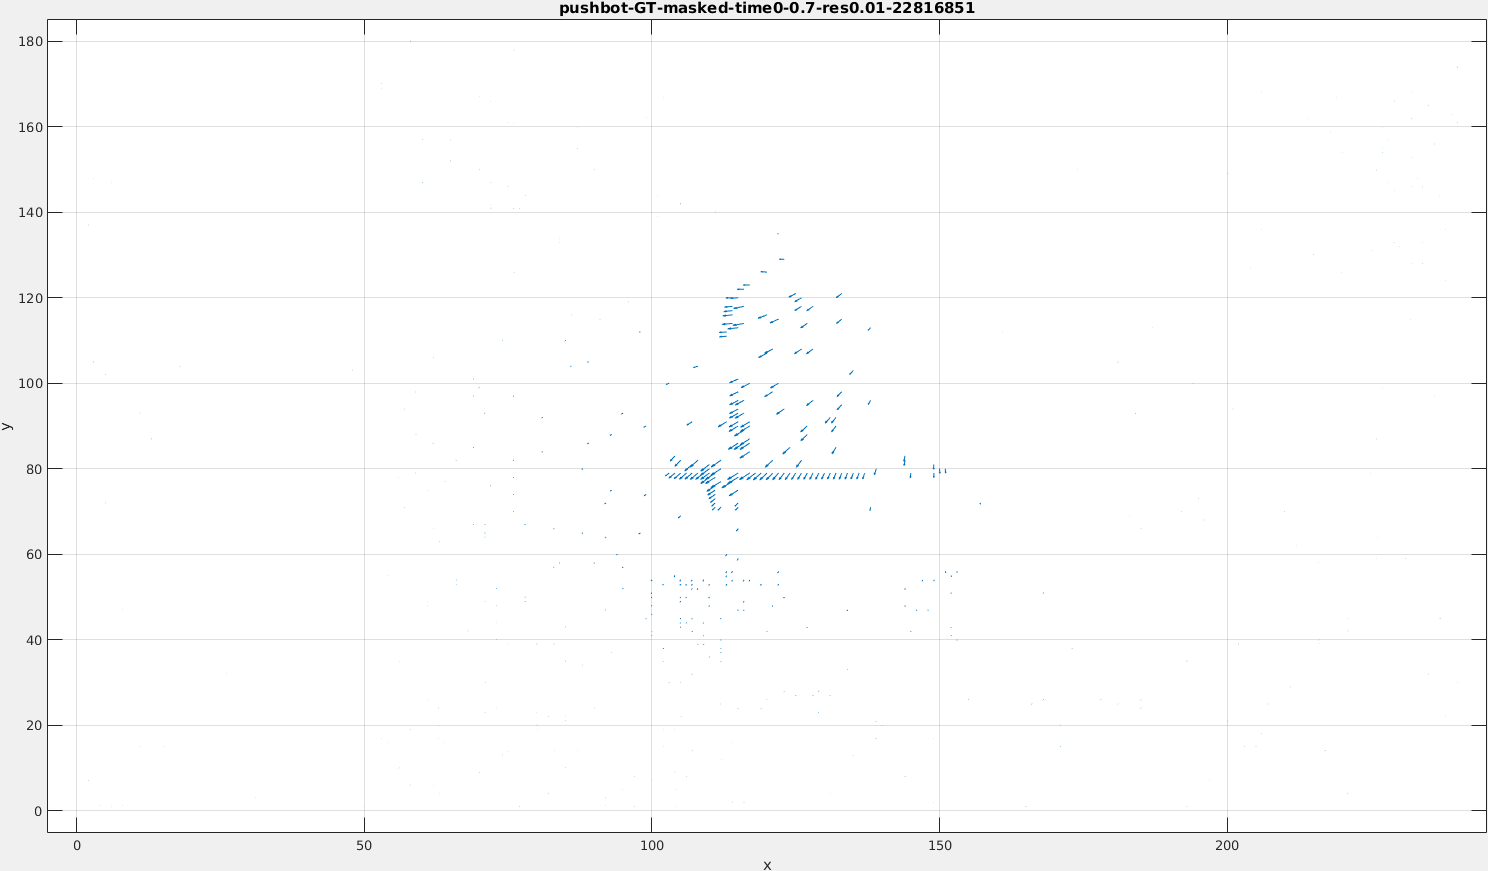
\includegraphics[height=.6\linewidth]{figs/pushbot/pushbot-GT-masked-2.png}
  \caption{}
\end{subfigure}
\caption[Second scene: Robot approaching the DVS sensor.]{Second scene: A small robot is approaching the DVS sensor. Figures (a) and (b) show the computed optical flow for the scene at two time steps. The masked flow fields are shown in Figures (c) and (d).
The corresponding ground truth is shown in Figures (e) and (f). Applying the same mask leads to Figures (g) and (h).
In the ground truth it can be observed that flow is directed to the bottom left of the frame (g)(h). 
In the computed flow, a horizontal edge at the bottom and a vertical edge at the left of the robot are clearly visible (c)(d).
The flow pointing from these edges indicates the direction of movement. 
It is most likely not pointing to the bottom left because of the missing normalization.}
\label{fig:pushbot-snapshots}
\end{figure}

\begin{table}[tb]
	\centering
		\begin{tabular}{lccccccc}
Scene & Setting & Matching & RMSE & MeanErr & MedianErr & Avg. Angle \\
\hline  \hline
pushbot & $1$ & direct & $94.54$ & $78.14$ & $69.79$ & -$101.37$ & \\
pushbot & $1$ & interp & $95.22$ & $78.85$ & $70.87$ &  & \\
pushbot & $2$ & direct & $94.54$ & $78.13$ & $69.83$ & -$101.27$ & \\
pushbot & $2$ & interp & $95.23$ & $78.87$ & $70.97$ &  & \\
pushbot & $3$ & direct & $92.84$ & $76.28$ & $66.58$ & -$103.75$ & \\
pushbot & $3$ & interp & $93.43$ & $76.85$ & $67.59$ &  & \\
pushbot & $4$ & direct & $92.79$ & $76.23$ & $66.73$ & -$103.29$ & \\
pushbot & $4$ & interp & $93.39$ & $76.80$ & $67.87$ &  & \\
pushbot & $5$ & direct & $94.05$ & $78.66$ & $71.46$ & -$101.32$ & \\
pushbot & $5$ & interp & $94.34$ & $78.96$ & $71.96$ &  & \\
pushbot & $6$ & direct & $94.12$ & $78.69$ & $71.32$ & -$101.33$ & \\
pushbot & $6$ & interp & $94.35$ & $78.96$ & $71.98$ &  & \\
pushbot & $7$ & direct & $93.73$ & $77.22$ & $68.16$ & -$99.43$ & \\
pushbot & $7$ & interp & $94.69$ & $78.23$ & $69.74$ &  & \\
pushbot & $8$ & direct & $93.74$ & $77.22$ & $68.27$ & -$99.06$ & \\
pushbot & $8$ & interp & $94.72$ & $78.26$ & $69.90$ &  & \\
pushbot & $9$ & direct & $91.69$ & $74.93$ & $64.18$ & -$102.94$ & \\
pushbot & $9$ & interp & $92.62$ & $75.91$ & $65.97$ &  & \\
pushbot & $10$ & direct & $91.66$ & $74.89$ & $64.03$ & -$102.48$ & \\
pushbot & $10$ & interp & $92.56$ & $75.84$ & $65.61$ &  & \\
pushbot & $11$ & direct & $92.64$ & $77.16$ & $69.08$ & -$100.00$ & \\
pushbot & $11$ & interp & $93.39$ & $77.89$ & $70.17$ &  & \\
pushbot & $12$ & direct & $92.71$ & $77.18$ & $69.12$ & -$99.99$ & \\
pushbot & $12$ & interp & $93.41$ & $77.89$ & $70.33$ &  & \\
		\end{tabular}
	\caption[Second scene: Comparison of angular errors for different parameters.]{Second scene: Comparison of angular errors for different parameters. The algorithm could not properly compute the flow for movement that is not perpendicular to the object's edges. This leads to a rather high angular error for all settings.}
	\label{tab:error_comparison_pushbot}
\end{table}


In the third investigated scene, the sensor itself is moved while observing the interior of a room (see Figure \ref{fig:skateboard-snapshots}). 
Due to the differences in how the flow was computed for the ground truth and the event-based optical flow, the angular errors are rather high as well in this scene.

The ground truth algorithm that works on dense images computes optical flow with rather homogeneous intensity for the whole scene.
In Figures \ref{fig:skateboard-snapshots1} and \ref{fig:skateboard-snapshots2} one can see that the edges of the walls are causing high responses and are clearly differentiable from the rest of the scene with the event-based optical flow.
Furthermore, it is notable that the algorithm was able to properly distinguish the rather high noise caused by the floor and actual edges in the scene.
The angular errors for this particular scene are rather high and the average angle of the computed flow varies significantly (see Table \ref{tab:error_comparison_skateboard}). 
One of the reasons for this is the rather high amount of noise, which partly leads to computed flow of arbitrary angles.
However, the figures of the masked ground truth and computed flow indicate a \edit{general concurrence.}{ was?}
Weighting the angular errors with the response intensity is likely to further reduce the error.


\begin{figure}[tb]
\centering
\begin{subfigure}{.45\textwidth}
  \centering
  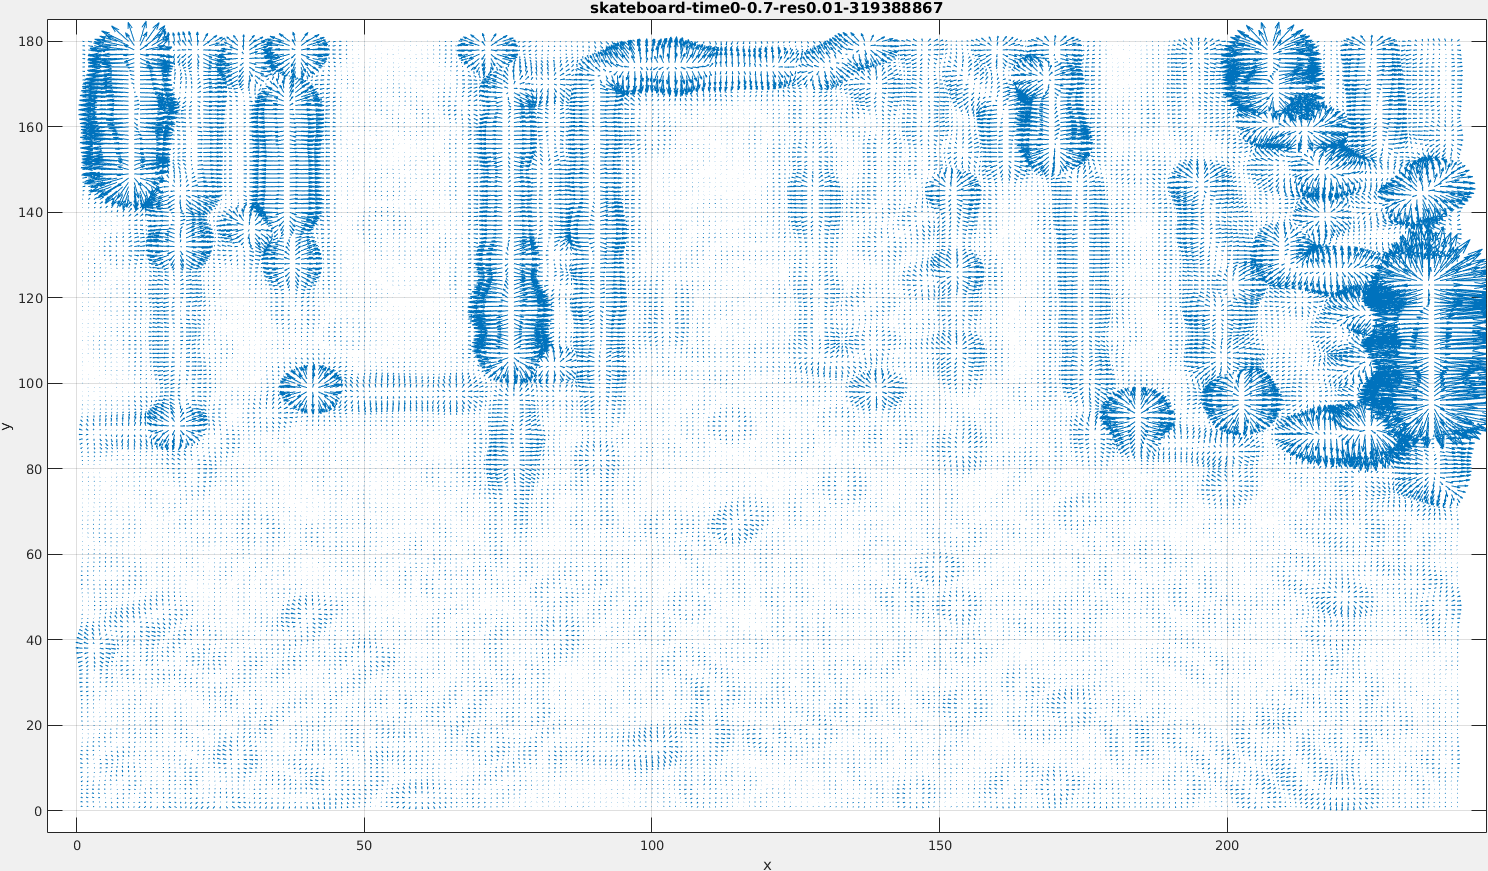
\includegraphics[height=.6\linewidth]{figs/skateboard/skateboard-1.png}
  \caption{}
  \label{fig:skateboard-snapshots1}
\end{subfigure}
\begin{subfigure}{.45\textwidth}
  \centering
  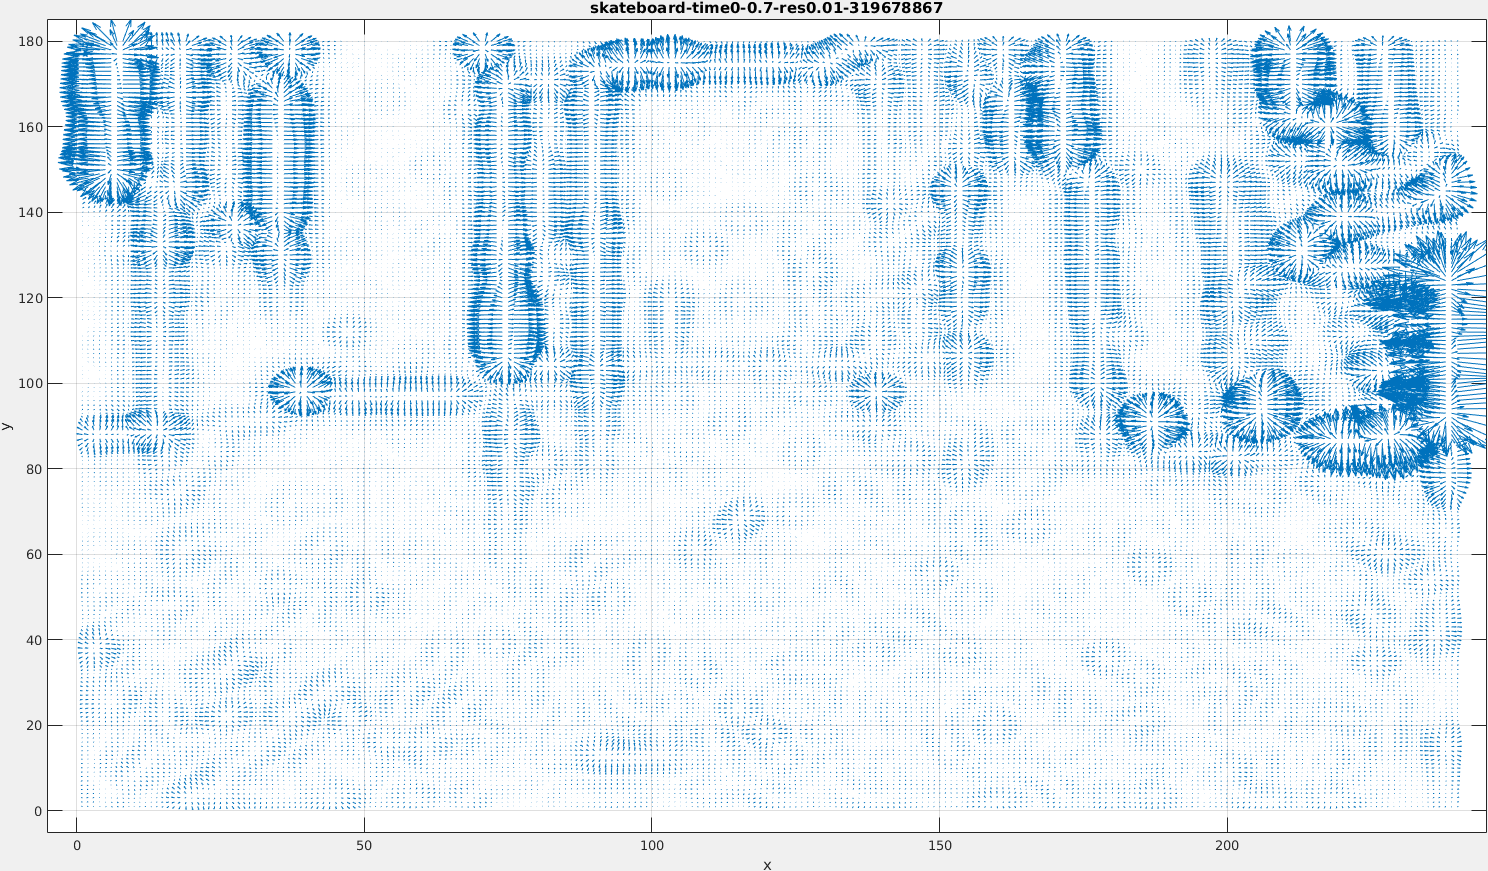
\includegraphics[height=.6\linewidth]{figs/skateboard/skateboard-2.png}
  \caption{}
  \label{fig:skateboard-snapshots2}
\end{subfigure}
\begin{subfigure}{.45\textwidth}
  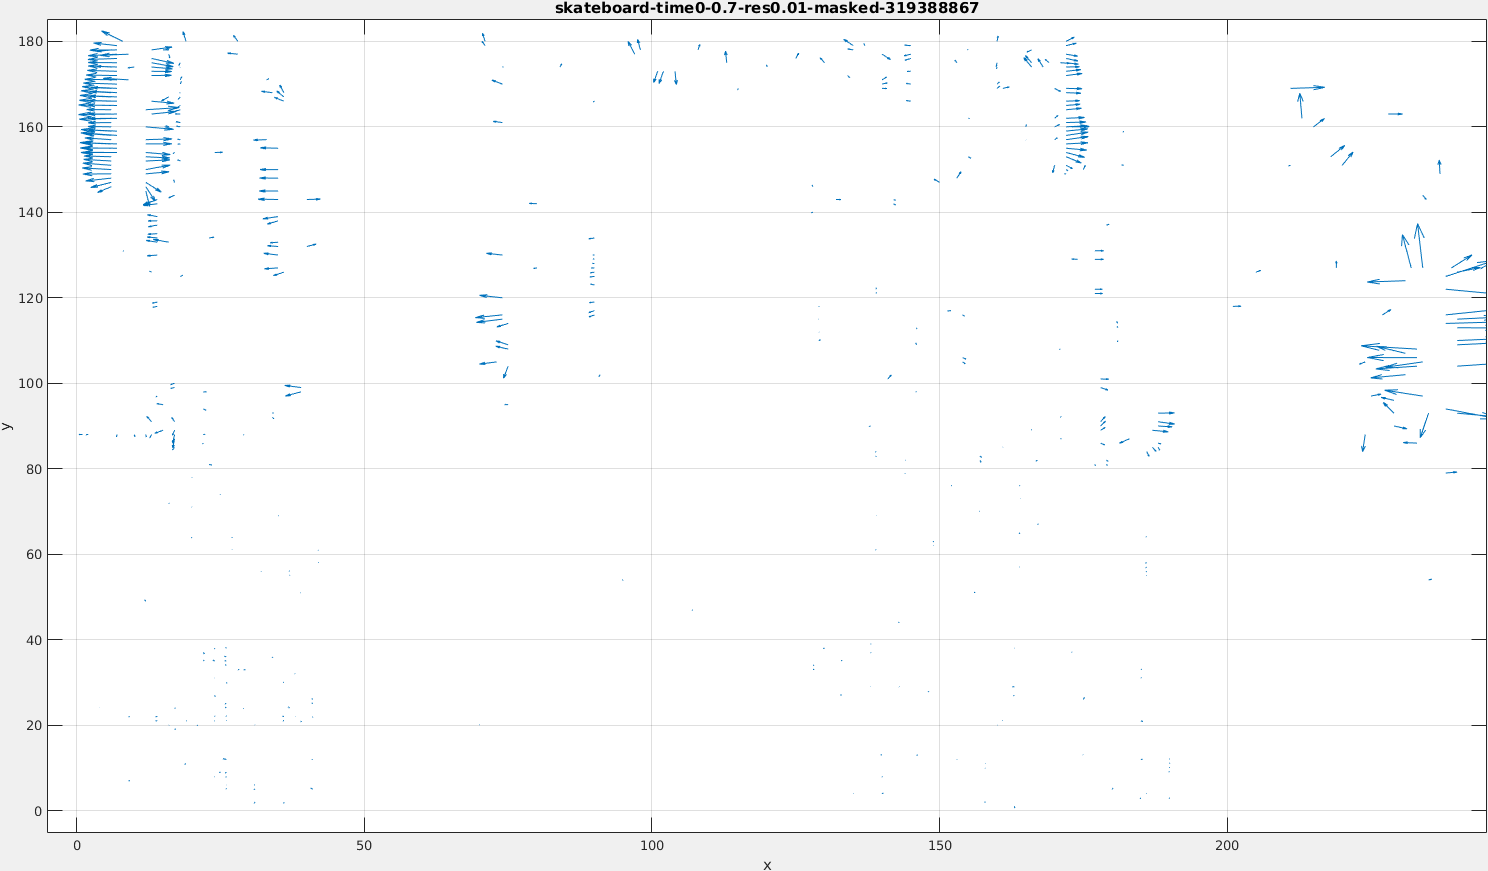
\includegraphics[height=.6\linewidth]{figs/skateboard/skateboard-masked-1.png}
  \caption{}
\end{subfigure}
\begin{subfigure}{.45\textwidth}
  \centering
  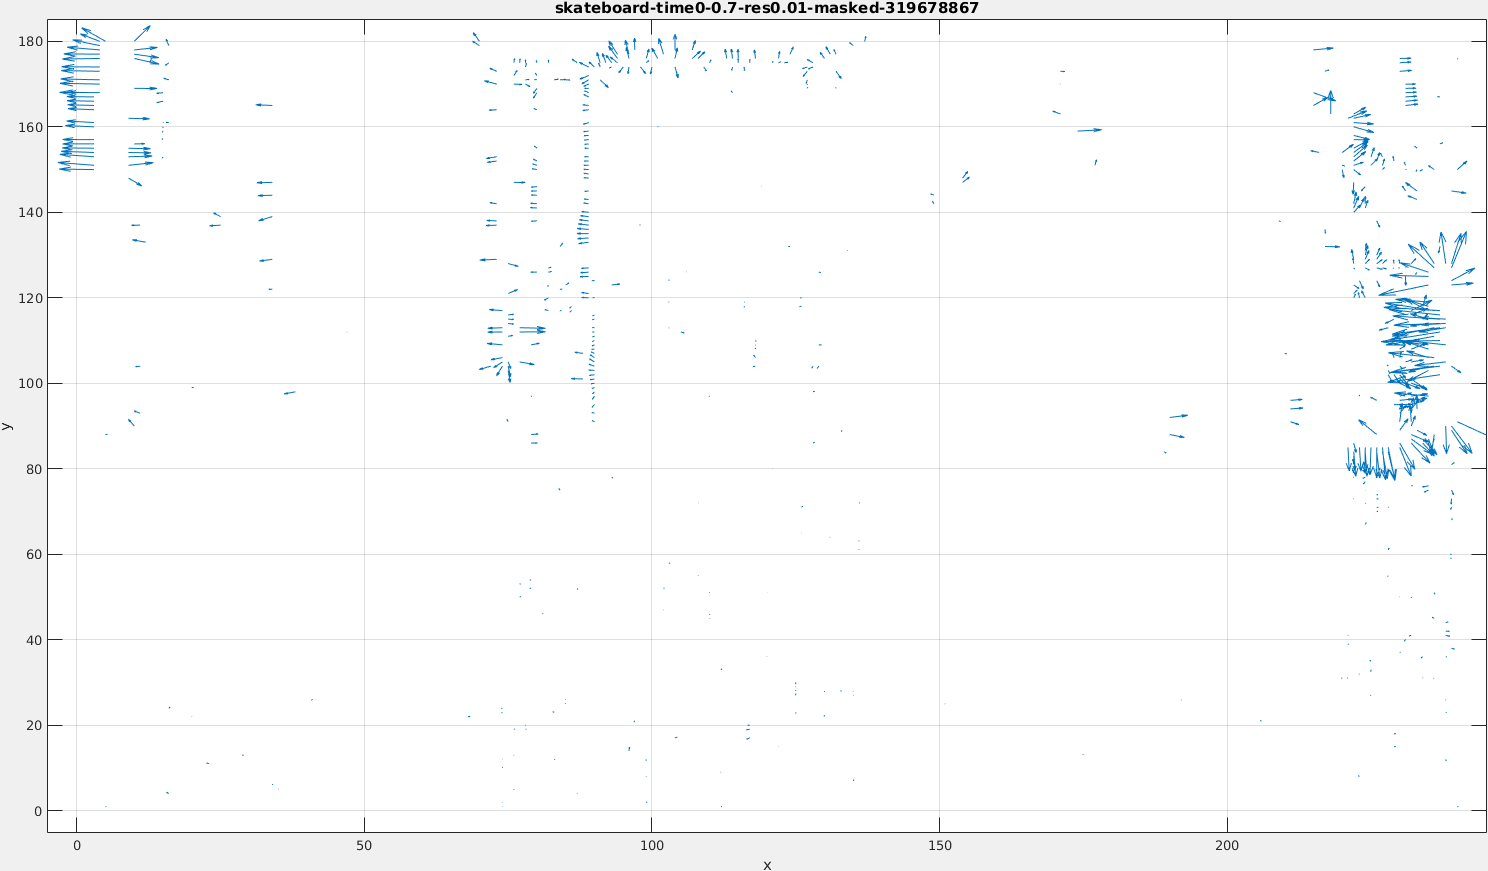
\includegraphics[height=.6\linewidth]{figs/skateboard/skateboard-masked-2.png}
  \caption{}
\end{subfigure}
\begin{subfigure}{.45\textwidth}
  \centering
  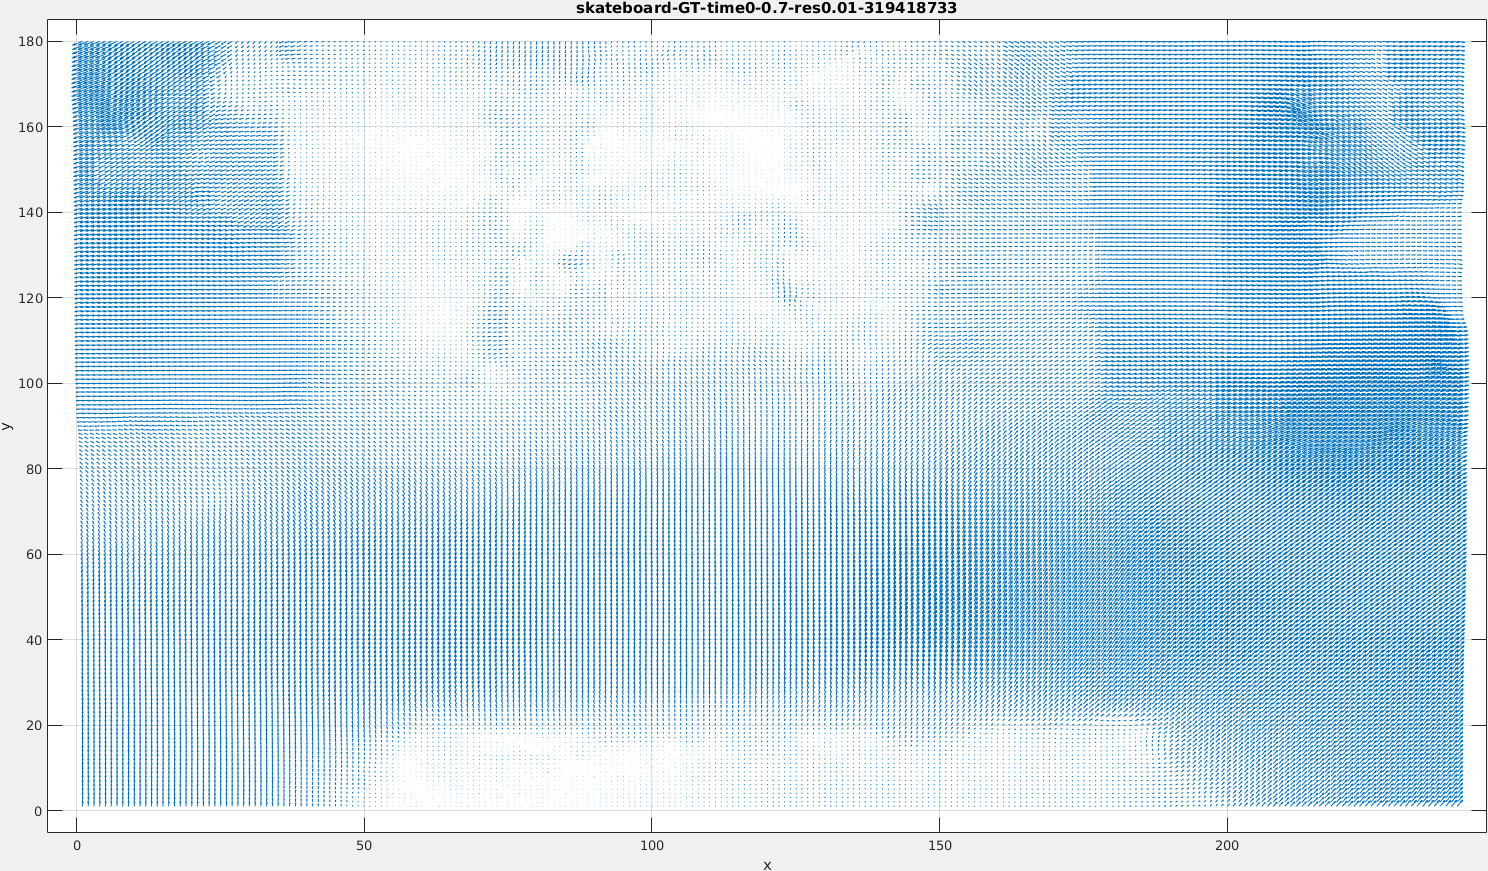
\includegraphics[height=.6\linewidth]{figs/skateboard/skateboard-GT-1.png}
  \caption{}
\end{subfigure}
\begin{subfigure}{.45\textwidth}
  \centering
  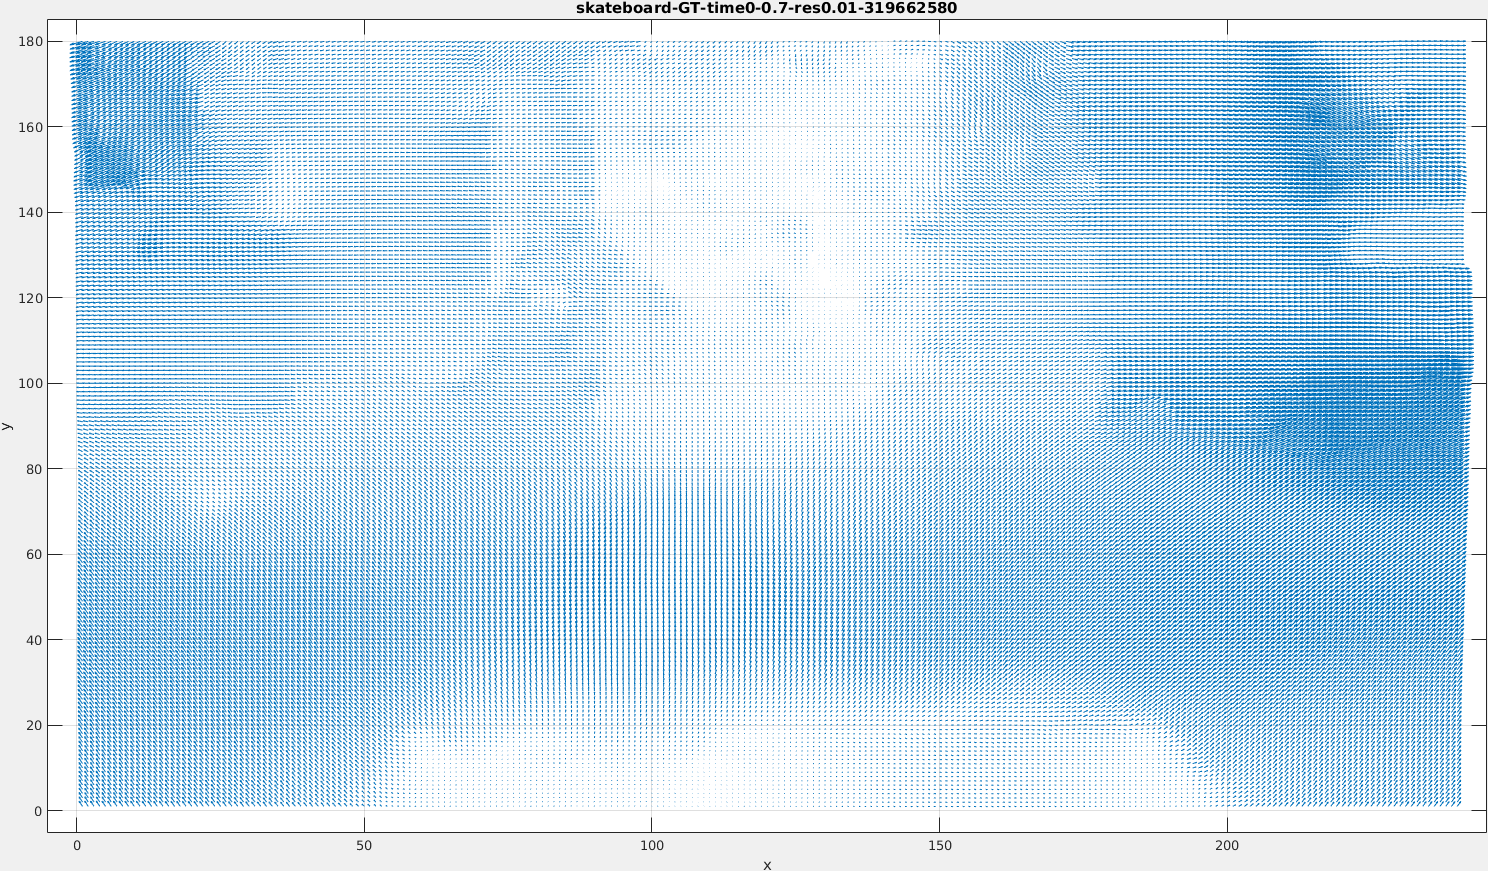
\includegraphics[height=.6\linewidth]{figs/skateboard/skateboard-GT-2.png}
  \caption{}
\end{subfigure}
\begin{subfigure}{.45\textwidth}
  \centering
  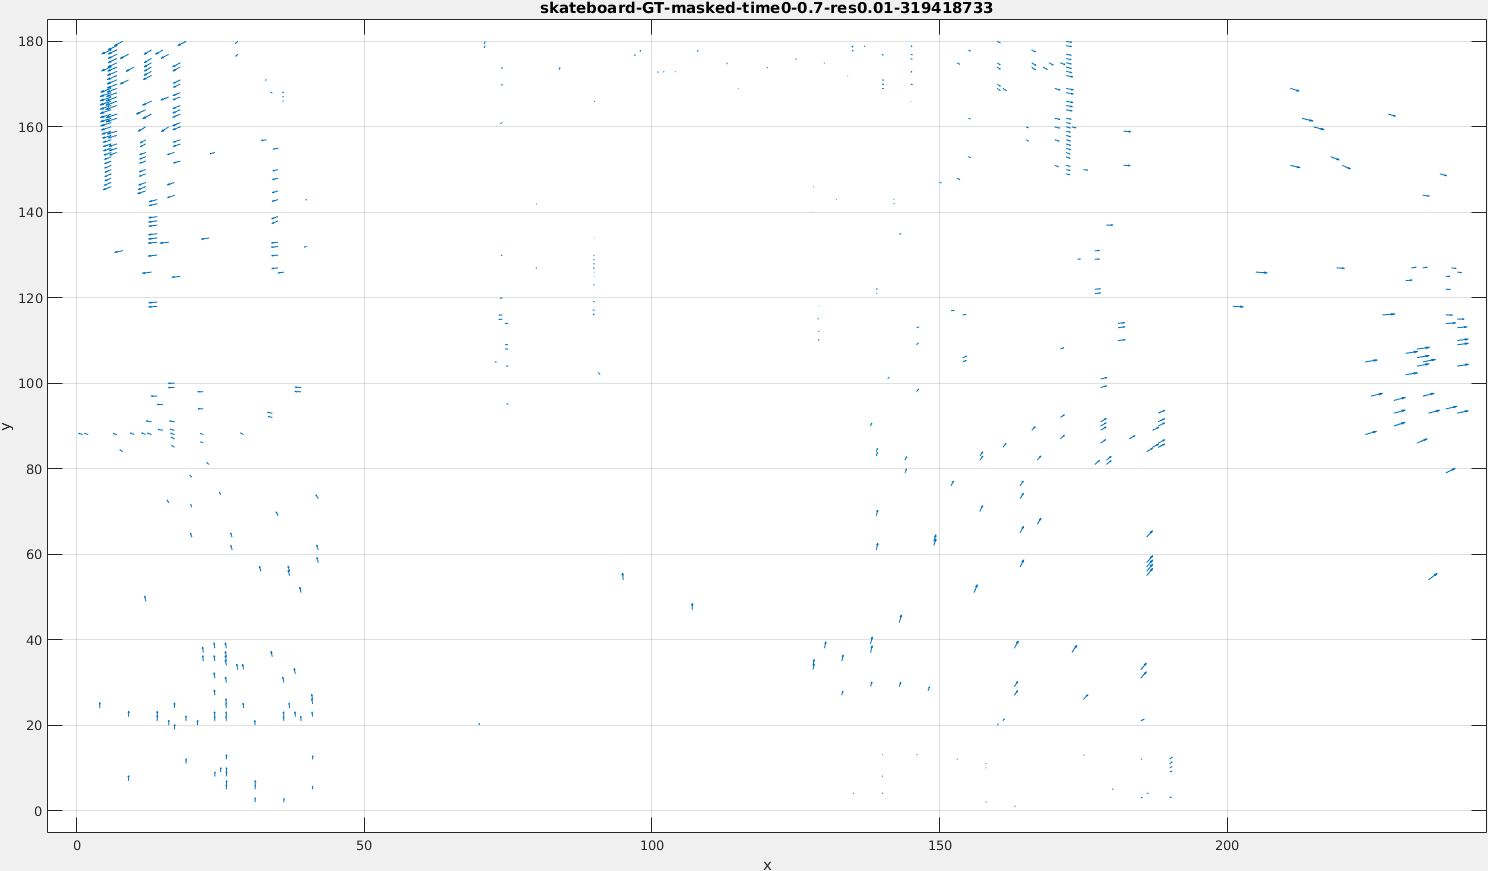
\includegraphics[height=.6\linewidth]{figs/skateboard/skateboard-GT-masked-1.png}
  \caption{}
\end{subfigure}
\begin{subfigure}{.45\textwidth}
  \centering
  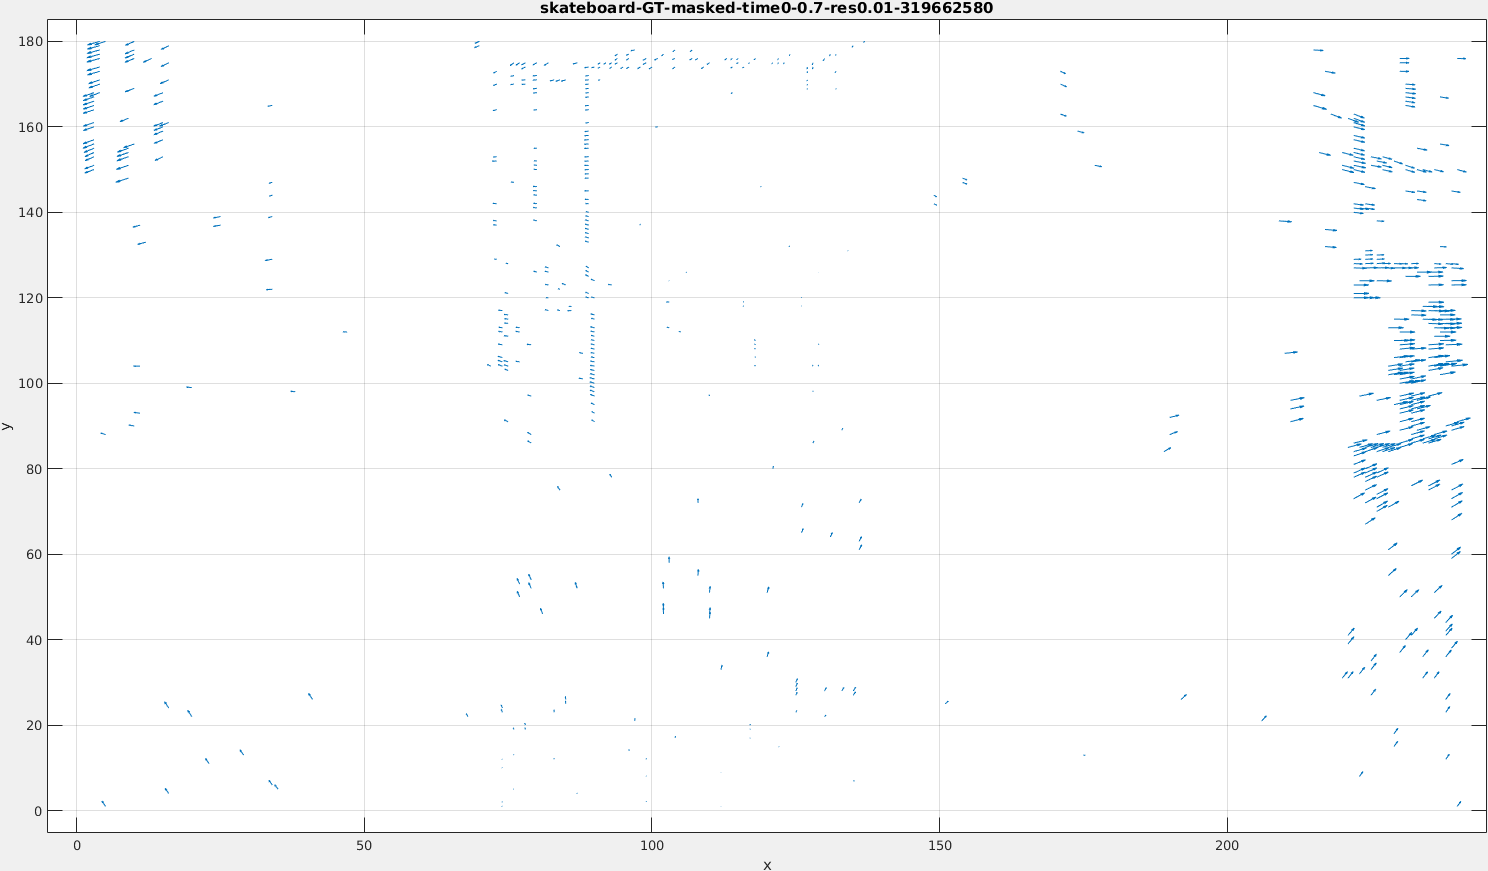
\includegraphics[height=.6\linewidth]{figs/skateboard/skateboard-GT-masked-2.png}
  \caption{}
\end{subfigure}
\caption[Third scene: Moving DVS sensor observing interior of a room.]{Third scene: Moving DVS sensor observing interior of a room. 
Figures (a) and (b) show the computed optical flow for the scene at two time steps. The masked flow fields are shown in Figures (c) and (d).
The corresponding ground truth is shown in Figures (e) and (f). 
Applying the same mask leads to Figures (g) and (h).

The computed flow clearly detects edges and dominant structures in the room (a)(b).
Trough masking, the visual similarities between the results (Figures (c) and (d)) and the ground truth ((g) and (h)) at the event locations become visible.
}
\label{fig:skateboard-snapshots}
\end{figure}

\begin{table}[tb]
	\centering
		\begin{tabular}{lccccccc}
Scene & Setting & Matching & RMSE & MeanErr & MedianErr & Avg. Angle \\
\hline  \hline
skateboard & $1$ & direct & $93.29$ & $75.56$ & $64.11$ & -$58.31$ & \\
skateboard & $1$ & interp & $92.90$ & $74.98$ & $62.95$ &  & \\
skateboard & $2$ & direct & $93.37$ & $75.82$ & $64.66$ & -$53.51$ & \\
skateboard & $2$ & interp & $93.01$ & $75.27$ & $63.60$ &  & \\
skateboard & $3$ & direct & $90.76$ & $72.70$ & $59.52$ & -$25.82$ & \\
skateboard & $3$ & interp & $90.38$ & $72.16$ & $58.44$ &  & \\
skateboard & $4$ & direct & $90.95$ & $73.07$ & $60.28$ & -$13.33$ & \\
skateboard & $4$ & interp & $90.60$ & $72.54$ & $59.14$ &  & \\
skateboard & $5$ & direct & $91.93$ & $73.85$ & $61.86$ & $58.94$ & \\
skateboard & $5$ & interp & $91.75$ & $73.47$ & $60.94$ &  & \\
skateboard & $6$ & direct & $91.78$ & $73.75$ & $61.77$ & $58.37$ & \\
skateboard & $6$ & interp & $91.58$ & $73.36$ & $61.02$ &  & \\
skateboard & $7$ & direct & $93.08$ & $75.39$ & $64.09$ & -$59.19$ & \\
skateboard & $7$ & interp & $92.65$ & $74.78$ & $62.82$ &  & \\
skateboard & $8$ & direct & $93.14$ & $75.63$ & $64.59$ & -$53.95$ & \\
skateboard & $8$ & interp & $92.73$ & $75.04$ & $63.33$ &  & \\
skateboard & $9$ & direct & $90.87$ & $72.91$ & $59.92$ & -$14.68$ & \\
skateboard & $9$ & interp & $90.46$ & $72.35$ & $58.71$ &  & \\
skateboard & $10$ & direct & $91.06$ & $73.28$ & $60.82$ & $2.49$ & \\
skateboard & $10$ & interp & $90.69$ & $72.73$ & $59.71$ &  & \\
skateboard & $11$ & direct & $92.06$ & $74.18$ & $62.78$ & $64.44$ & \\
skateboard & $11$ & interp & $91.92$ & $73.85$ & $61.97$ &  & \\
skateboard & $12$ & direct & $91.91$ & $74.09$ & $62.62$ & $64.99$ & \\
skateboard & $12$ & interp & $91.77$ & $73.75$ & $61.84$ &  & \\
		\end{tabular}
	\caption[Third scene: Comparison of angular errors for different parameters.]{Third scene: Comparison of angular errors for different parameters. 
	Due to a high degree of noise, the angular error is rather high and the average angle greatly varies.}
	\label{tab:error_comparison_skateboard}
\end{table}



The following evaluations have been conducted with a synthetically created set of event data and ground truths.
Due to the method of creating the scenes with a 3D software, the scenes are rather short ($0.3$ s) and the depicted geometrical objects move faster.
The temporal resolution for the filtering is increased in order to deal with the higher number of events due to the fast movement.
The responses of the event-based flow are very low in the three investigated cases. 
This is likely caused by the very high movement speed of the observed object.
The Gabor filters we used in the experiments have a fixed speed selectivity. 
If the movement speed of objects in the scene differs a lot from this speed, the filter response is rather low.
To still properly visually compare the computed flow fields, we magnify the values in the quiver plot by $10$ for the 'square1.2' and 'square2' scene, and by $100$ for the 'baelle' scene.


In the first synthetic scene, a square is linearly moving from the middle of the window to the lower right corner of the window with constant speed.
It is interesting to note that the algorithm fails to recognize the right and bottom edge of the square (see Figure \ref{fig:square12-snapshots}).
This is likely caused by the perfectly aligned simultaneous movement off all pixels on the outer edges.
%Explain further
The object is moving in a direction not perpendicular to its edges.
As in the previous scenes, the angular error is likely increased due to the missing normalization and amounts to about $40^\circ$ for different measurement metrics (see Table \ref{tab:error_comparison_square12}). 
 
Furthermore, the effects of the aperture are visible again at the outer corners of the edges.

\begin{figure}[tb]
\centering
\begin{subfigure}{.45\textwidth}
  \centering
  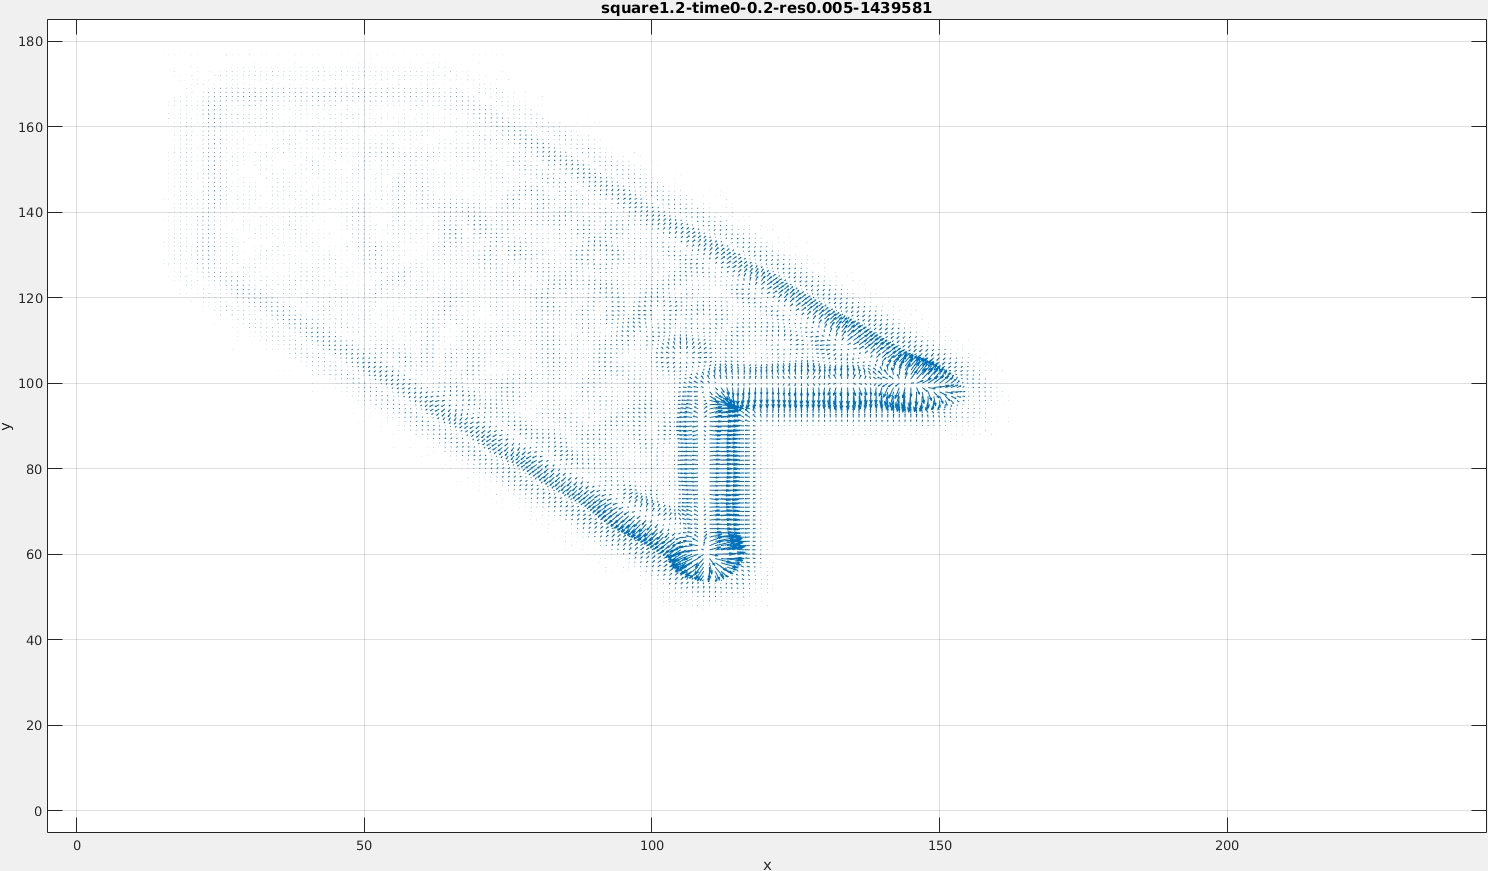
\includegraphics[height=.6\linewidth]{figs/square12/square12-1.png}
  \caption{}
\end{subfigure}
\begin{subfigure}{.45\textwidth}
  \centering
  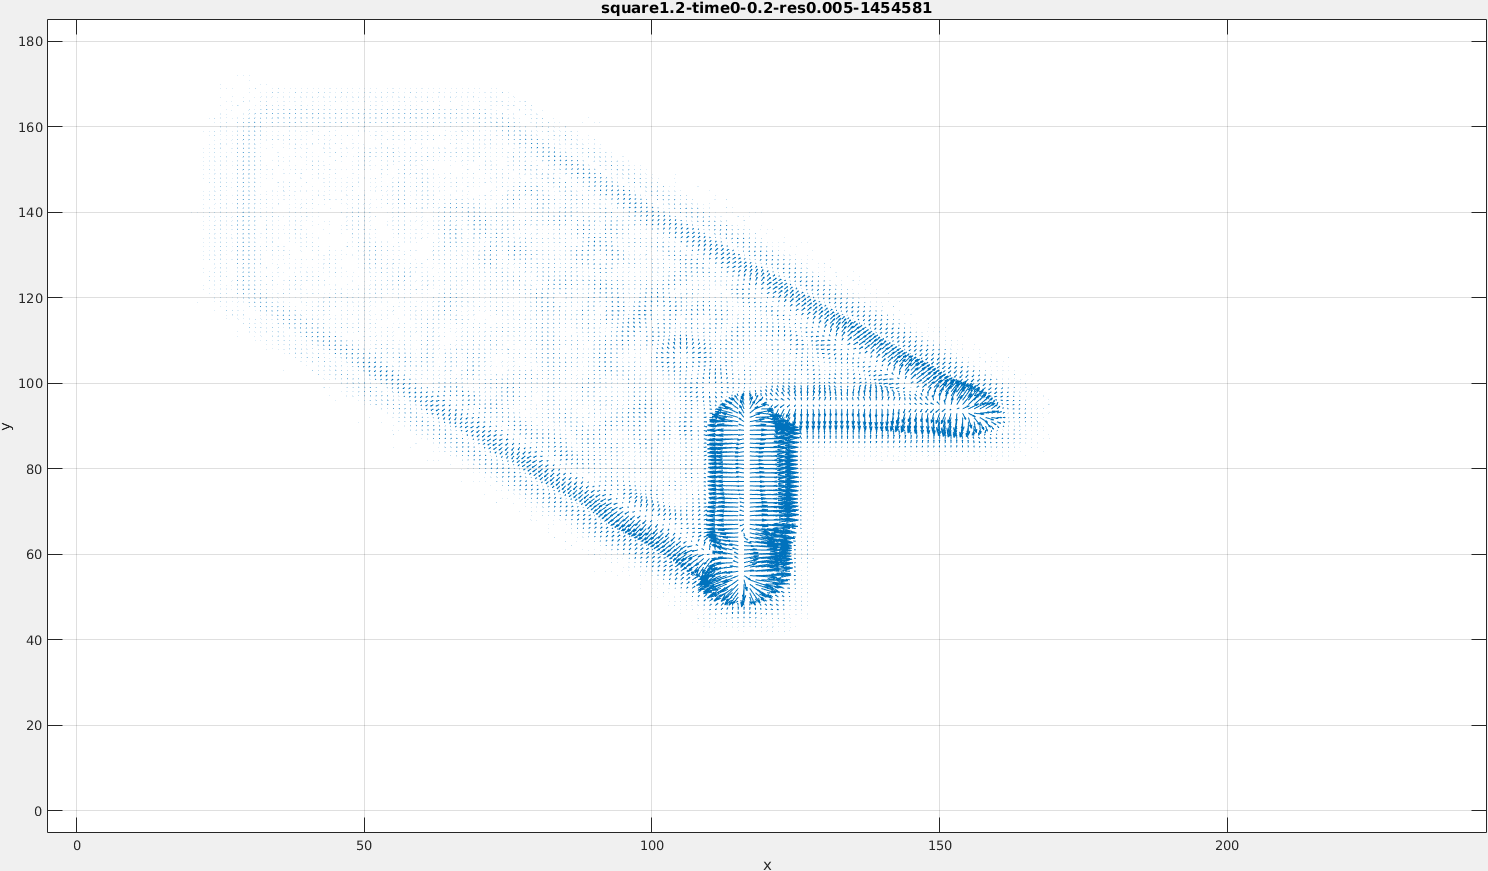
\includegraphics[height=.6\linewidth]{figs/square12/square12-2.png}
  \caption{}
\end{subfigure}
\begin{subfigure}{.45\textwidth}
  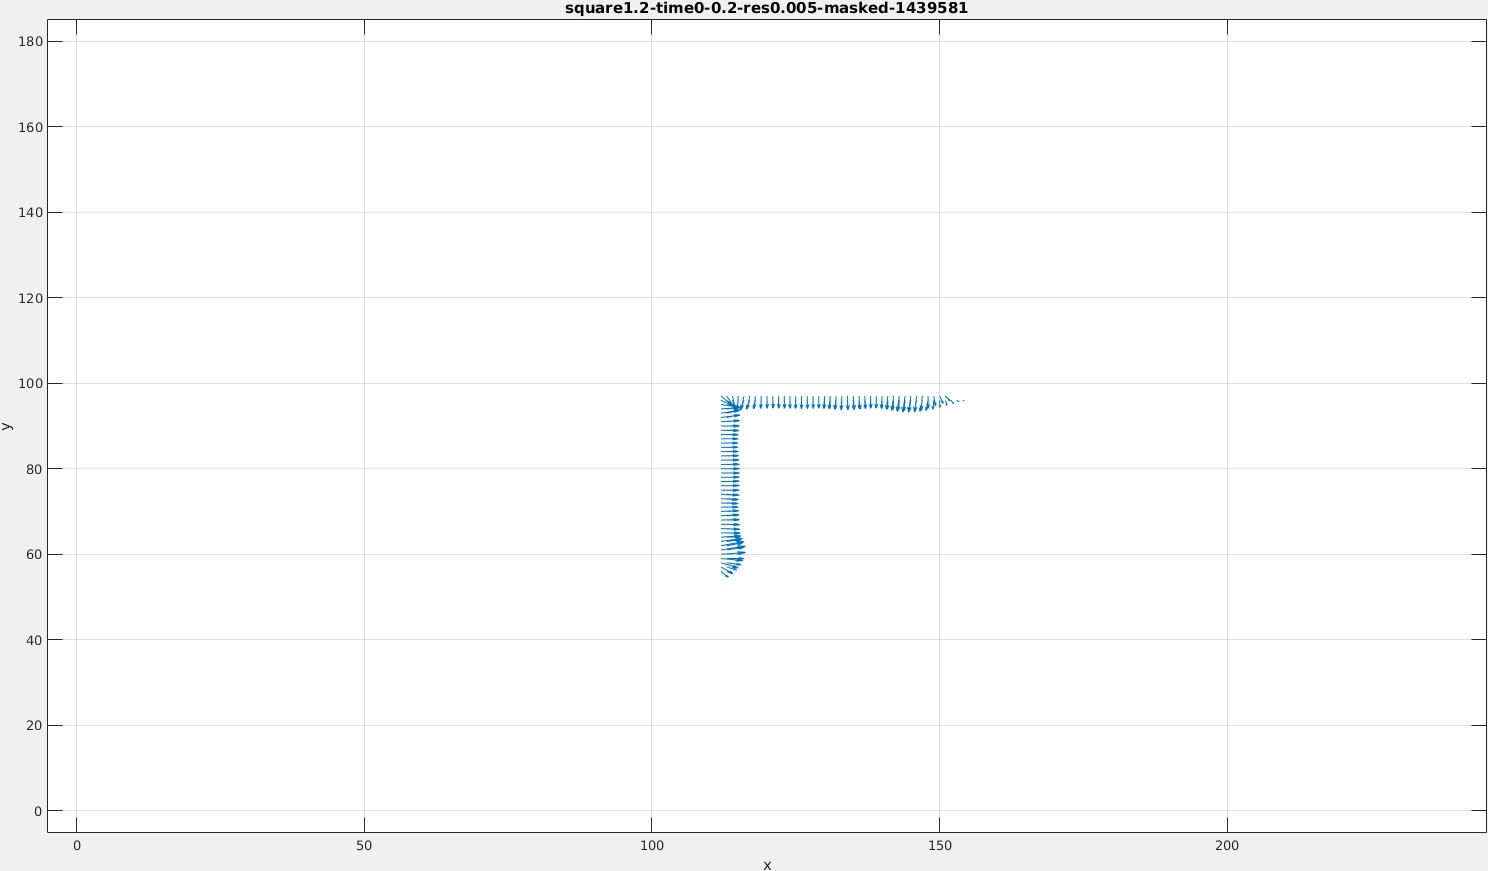
\includegraphics[height=.6\linewidth]{figs/square12/square12-masked-1.png}
  \caption{}
\end{subfigure}
\begin{subfigure}{.45\textwidth}
  \centering
  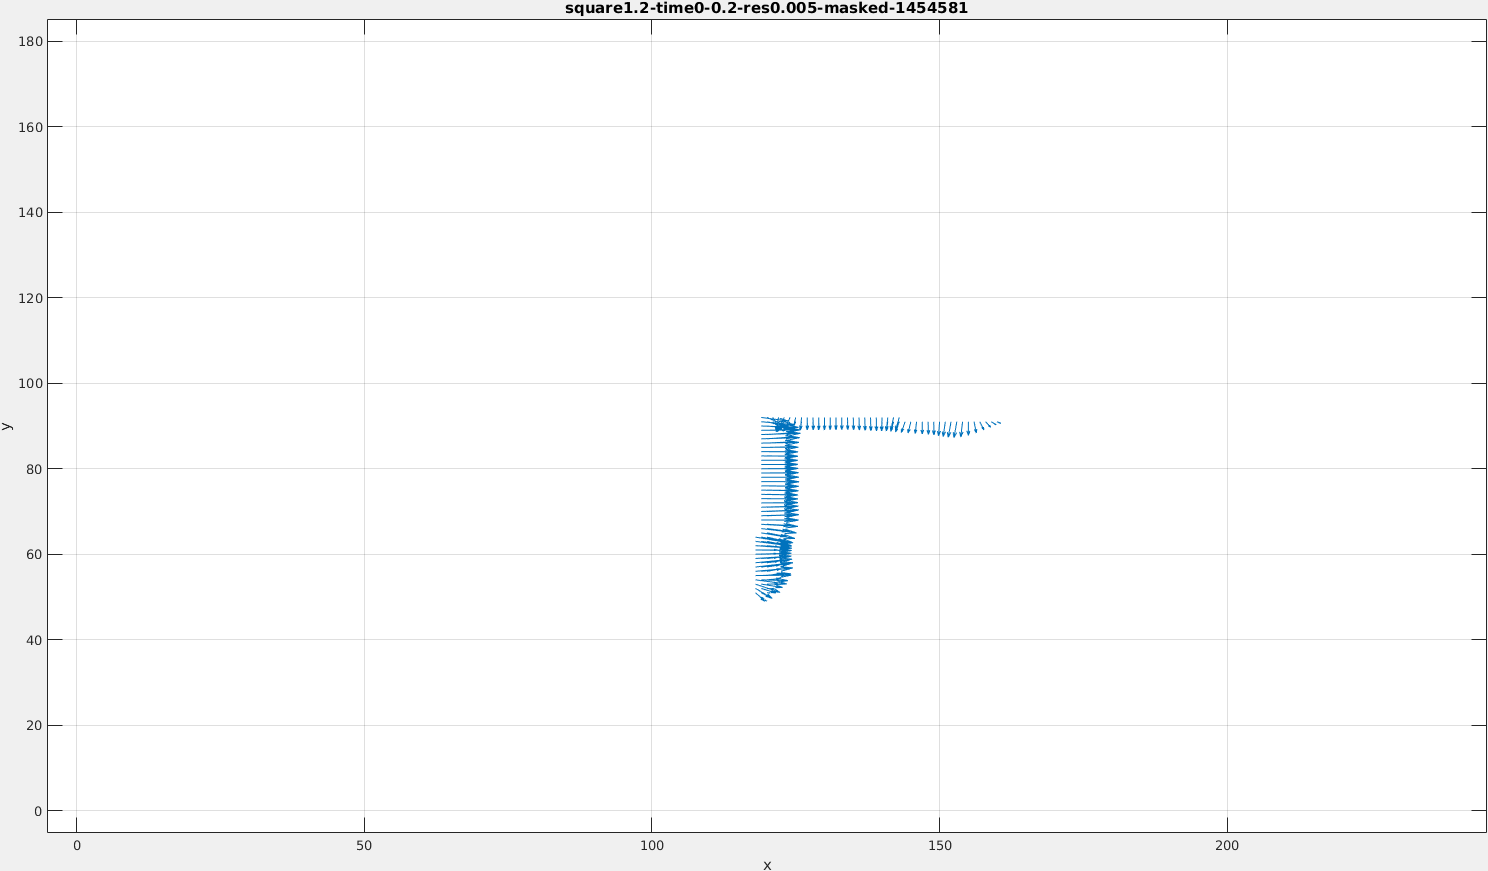
\includegraphics[height=.6\linewidth]{figs/square12/square12-masked-2.png}
  \caption{}
\end{subfigure}
\begin{subfigure}{.45\textwidth}
  \centering
  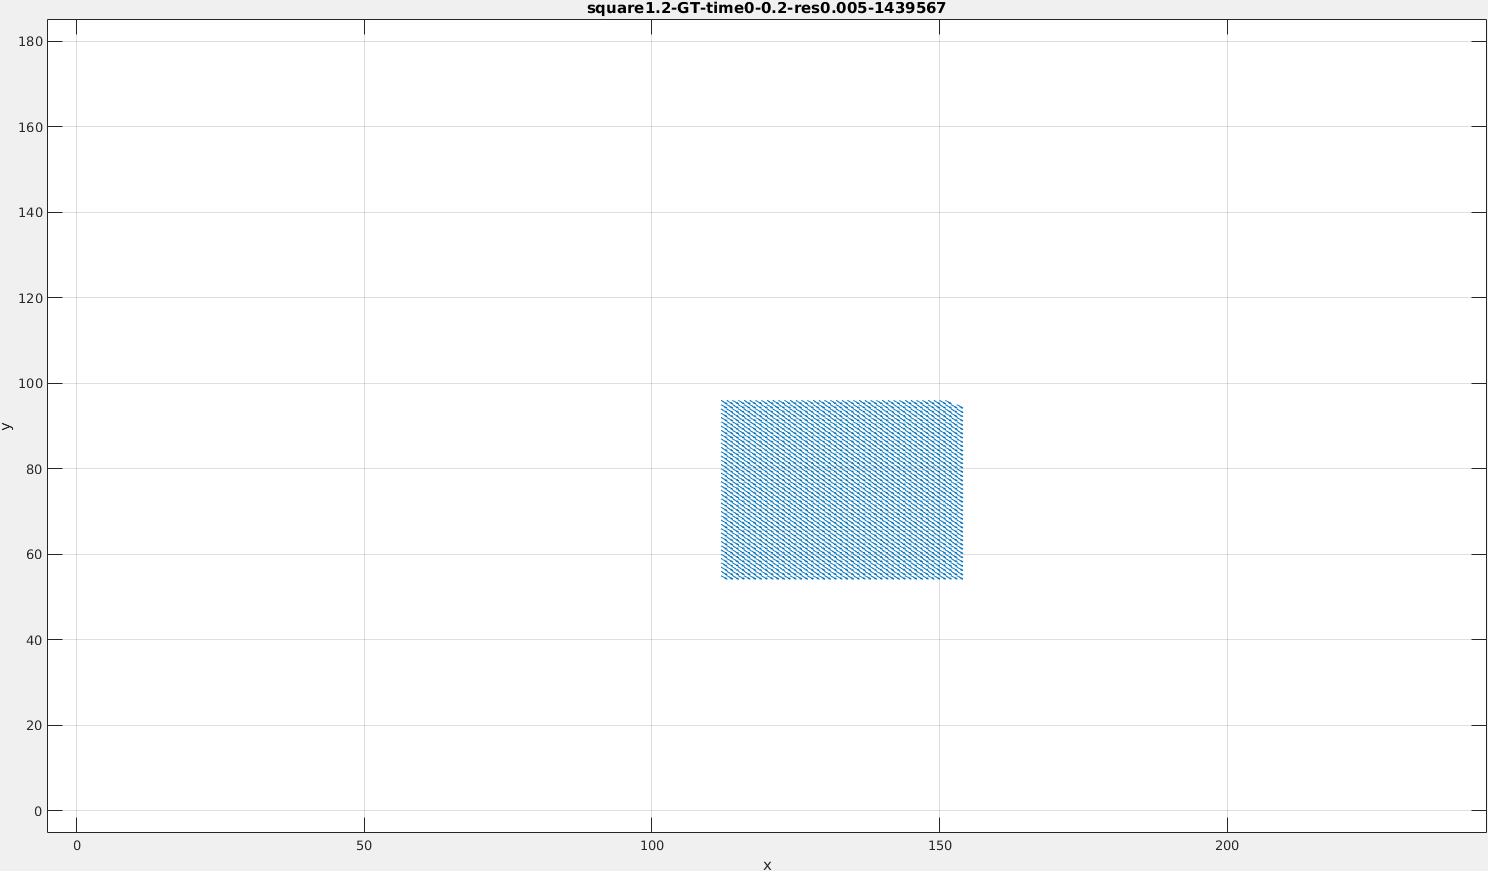
\includegraphics[height=.6\linewidth]{figs/square12/square12-GT-1.png}
  \caption{}
\end{subfigure}
\begin{subfigure}{.45\textwidth}
  \centering
  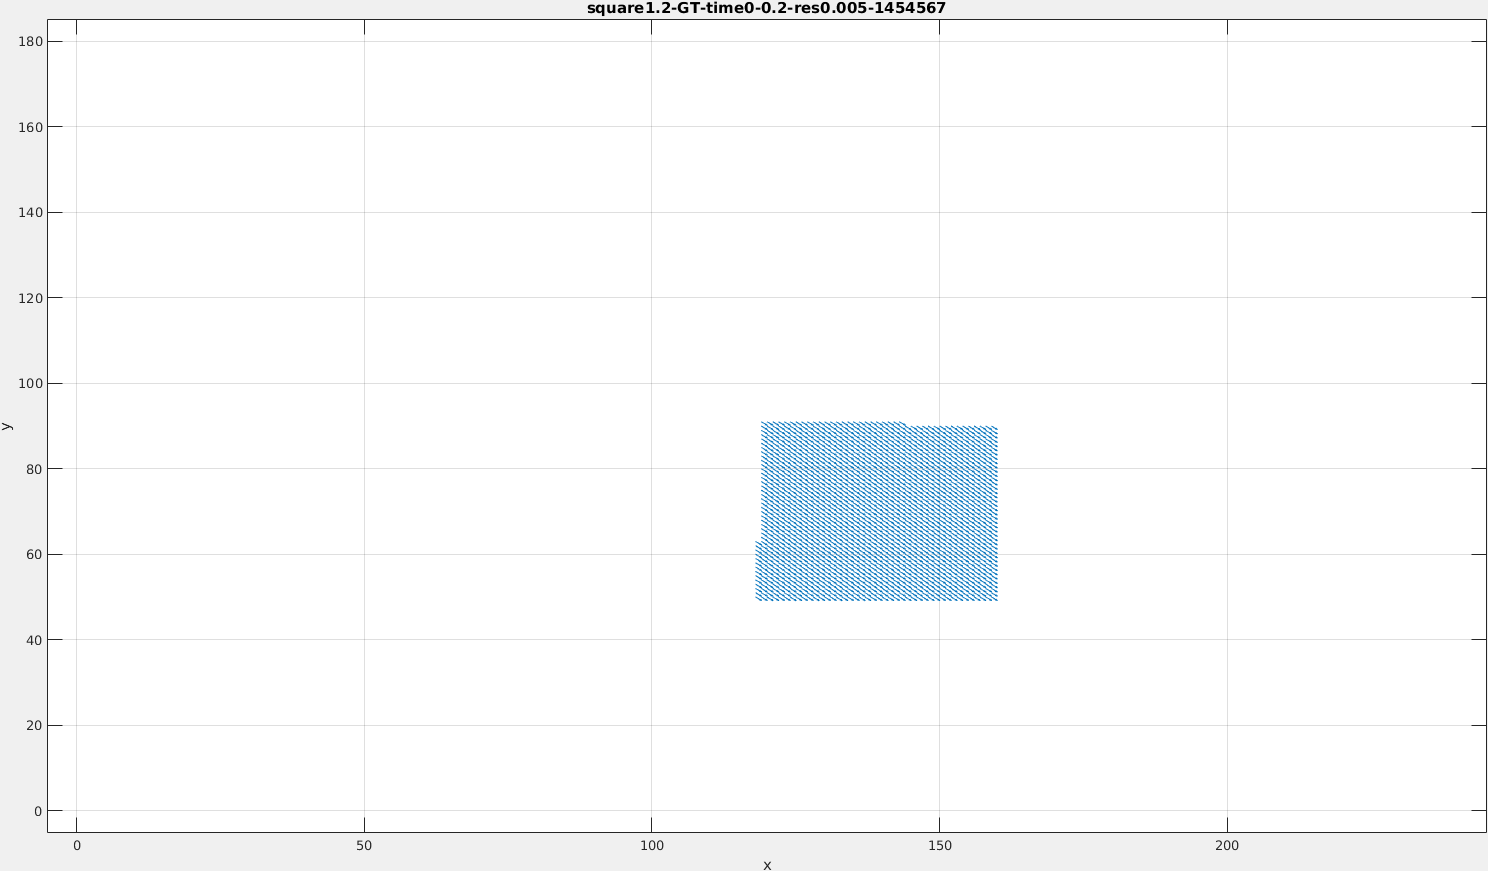
\includegraphics[height=.6\linewidth]{figs/square12/square12-GT-2.png}
  \caption{}
\end{subfigure}
\begin{subfigure}{.45\textwidth}
  \centering
  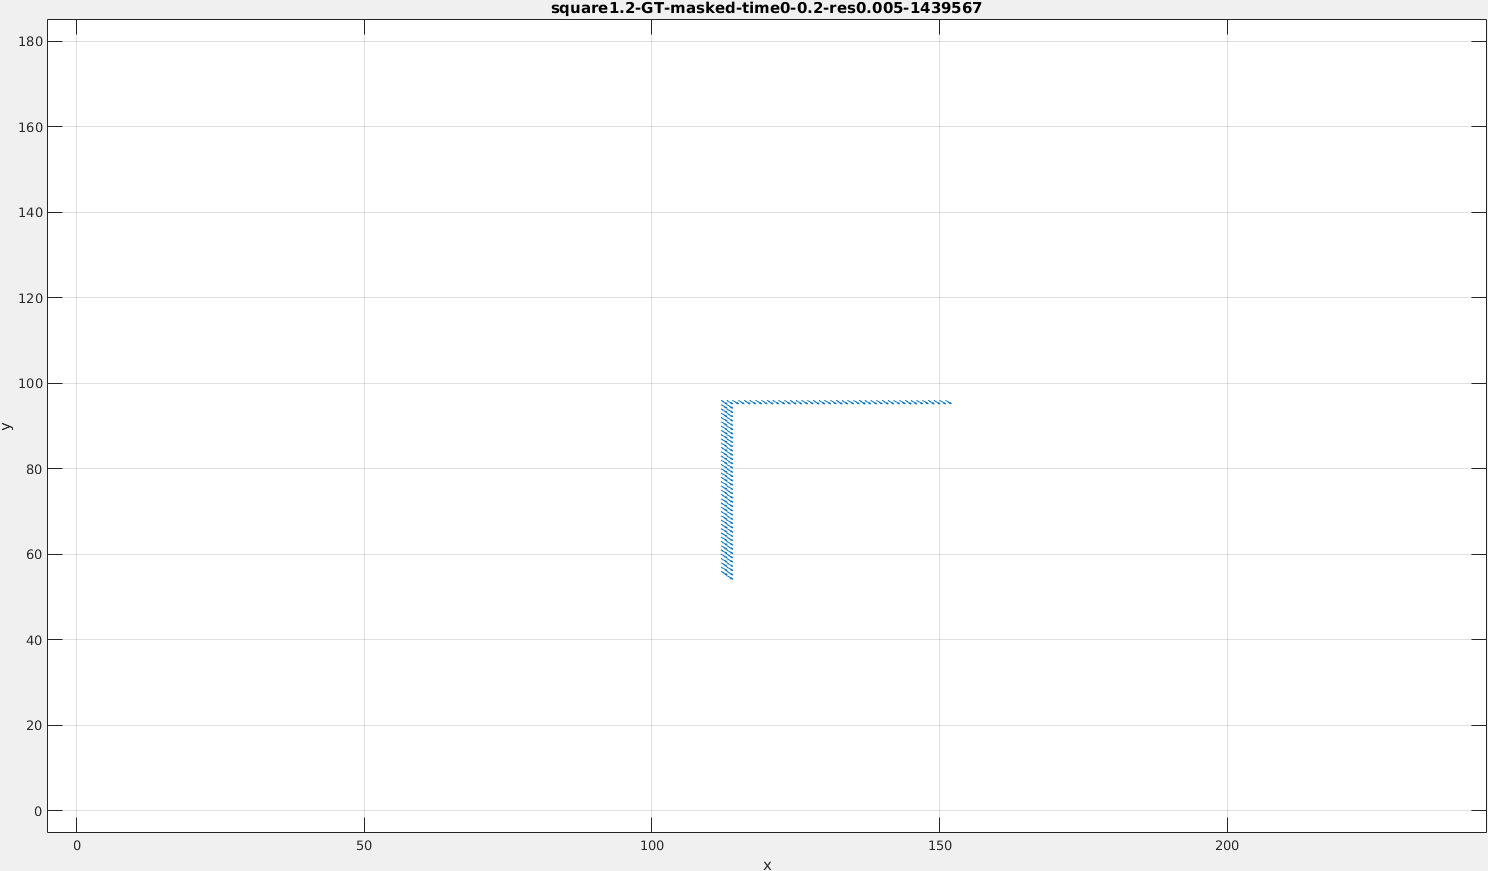
\includegraphics[height=.6\linewidth]{figs/square12/square12-GT-masked-1.png}
  \caption{}
\end{subfigure}
\begin{subfigure}{.45\textwidth}
  \centering
  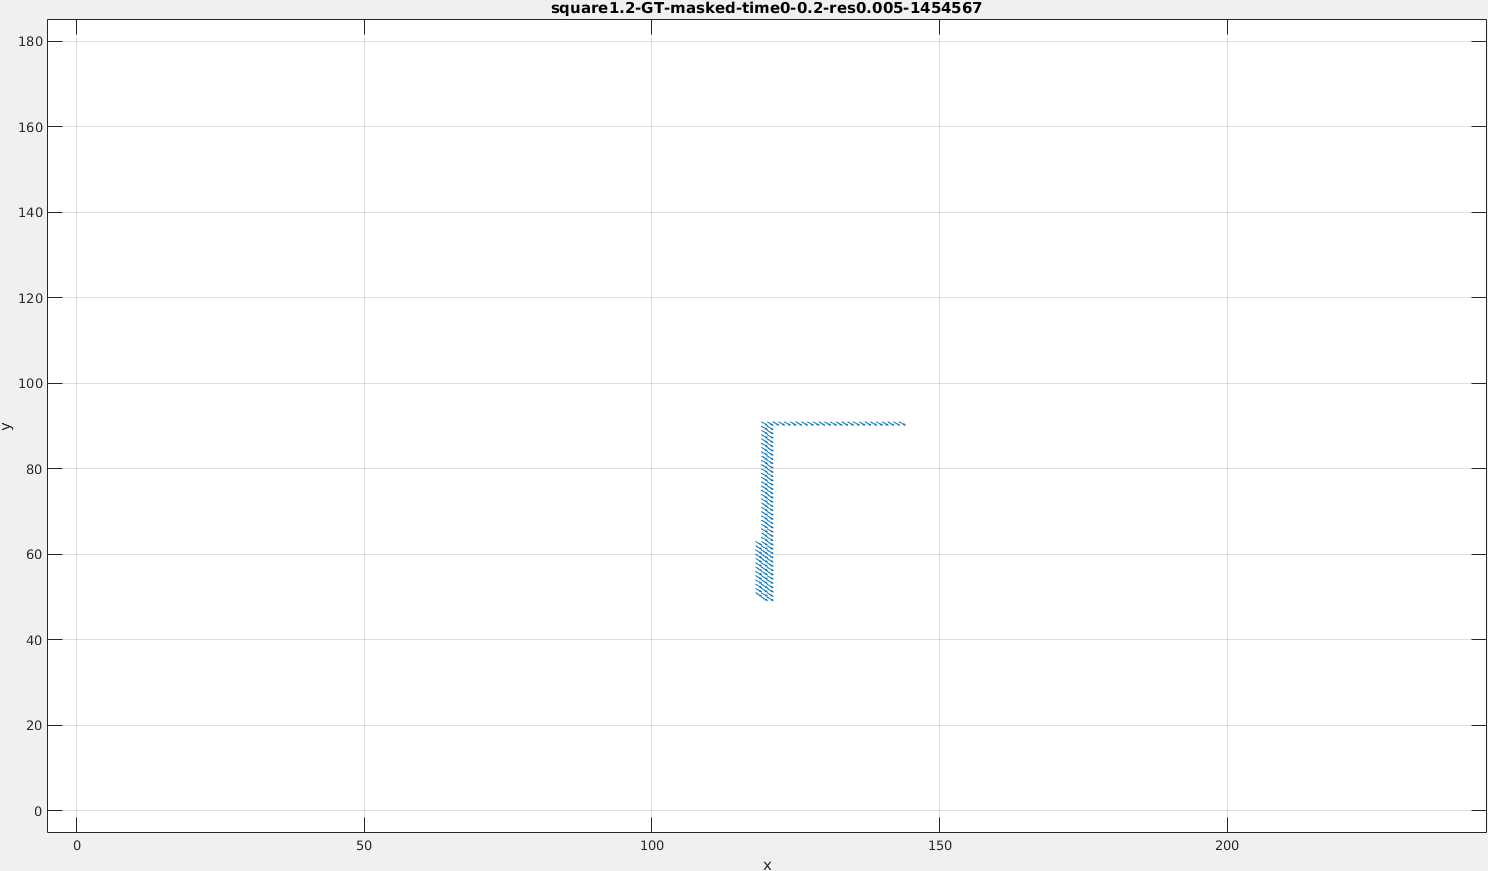
\includegraphics[height=.6\linewidth]{figs/square12/square12-GT-masked-2.png}
  \caption{}
\end{subfigure}
\caption[Fourth scene: Synthetic data of a linearly moving square.]{Fourth scene: Synthetic data of a linearly moving square.
Figures (a) and (b) show the computed optical flow for the scene at two time steps. The masked flow fields are shown in Figures (c) and (d).
The corresponding ground truth is shown in Figures (e) and (f). Applying the same mask leads to Figures (g) and (h).
Due to the synthetic nature of the data, all pixels of the outer edges moved simultaneously.
This leads to our algorithm failing to recognize the edges at all.
The effects of the aperture problem are visible a the right and bottom corner of the edges in Figures (a) and (b).
}
\label{fig:square12-snapshots}
\end{figure}

\begin{table}[tb]
	\centering
		\begin{tabular}{lccccccc}
Scene & Setting & Matching & RMSE & MeanErr & MedianErr & Avg. Angle \\
\hline  \hline
square1.2 & $13$ & direct & $42.71$ & $40.86$ & $39.17$ & -$37.72$ & \\
square1.2 & $13$ & interp & $42.84$ & $40.89$ & $39.17$ &  & \\
square1.2 & $14$ & direct & $42.55$ & $40.78$ & $39.10$ & -$38.04$ & \\
square1.2 & $14$ & interp & $42.65$ & $40.81$ & $39.11$ &  & \\
		\end{tabular}
	\caption[Fourth scene: Comparison of angular errors for different parameters.]{Fourth scene: Comparison of angular errors for different parameters.
	The angular error is rather high for all measurement metrics.
	A likely reason is the movement direction of the square, which is non-perpendicular to its edges.}
	\label{tab:error_comparison_square12}
\end{table}

In the second synthetic scene, a square is moving in a circular trajectory (see Figure \ref{fig:square2-snapshots}).
The square is moving such that its front edge is always perpendicular to the direction of movement.
In comparison to the fourth scene, the angular error is greatly reduced, which emphasizes the effect of the normalization (see Table \ref{tab:error_comparison_square2}).
Again, the algorithm fails to recognize the outer edge in movement direction.

\begin{figure}[tb]
\centering
\begin{subfigure}{.45\textwidth}
  \centering
  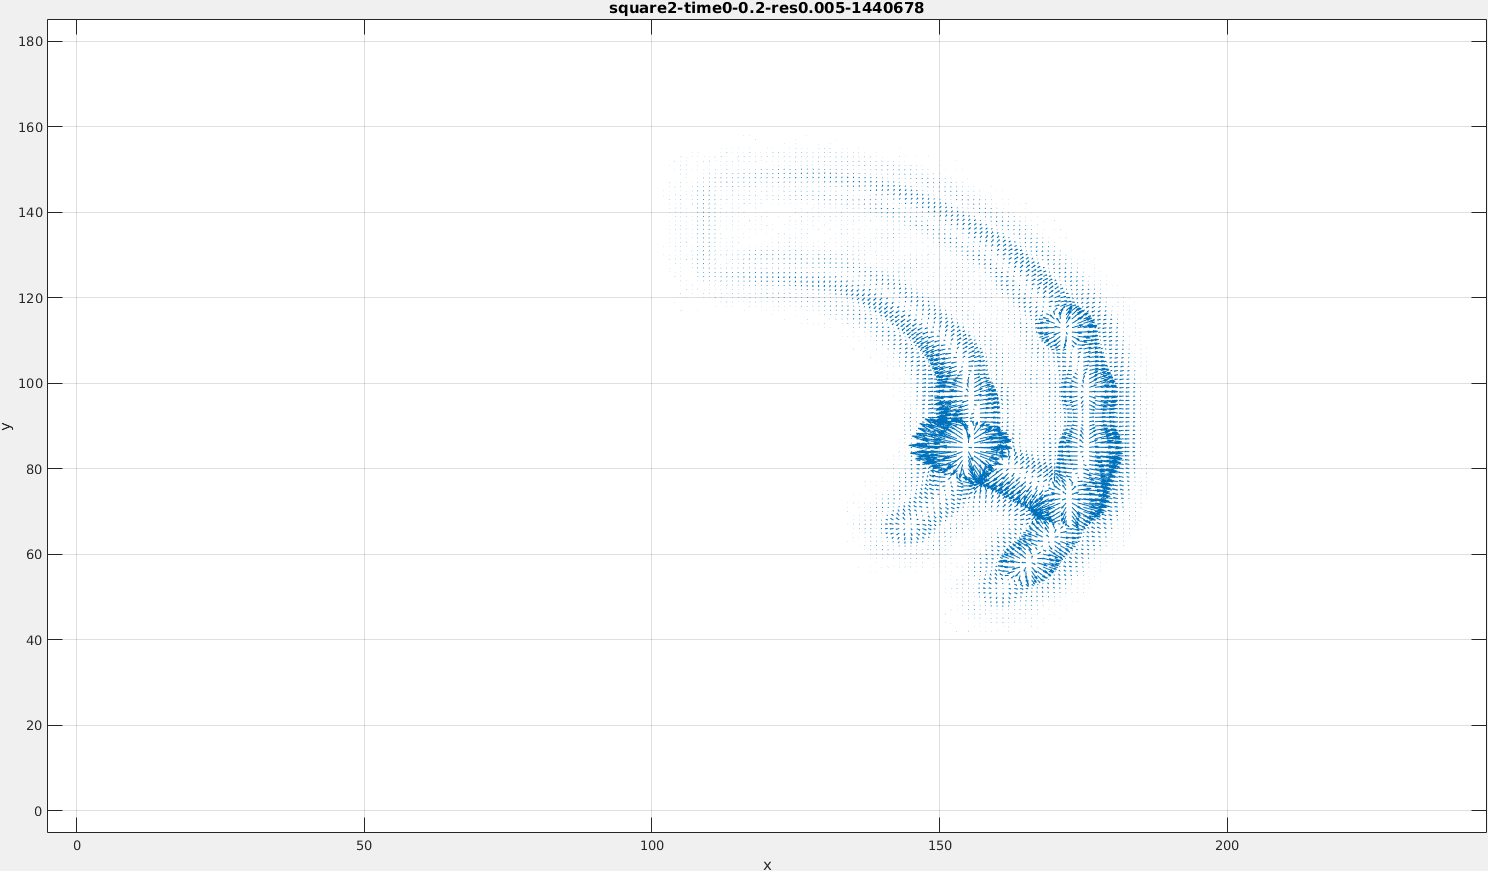
\includegraphics[height=.6\linewidth]{figs/square2/square2-1.png}
  \caption{}
\end{subfigure}
\begin{subfigure}{.45\textwidth}
  \centering
  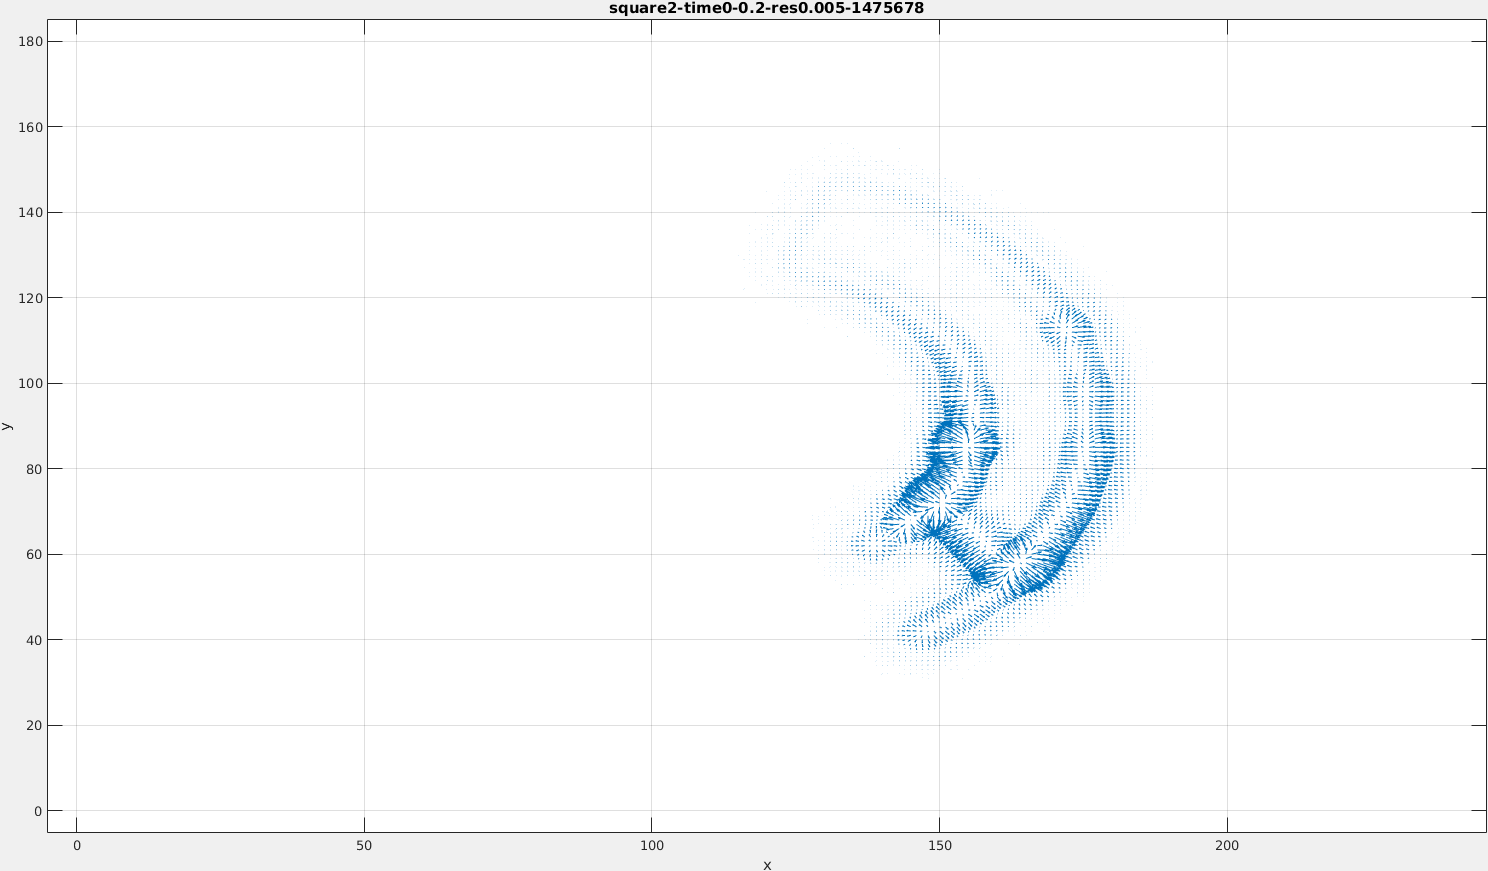
\includegraphics[height=.6\linewidth]{figs/square2/square2-2.png}
  \caption{}
\end{subfigure}
\begin{subfigure}{.45\textwidth}
  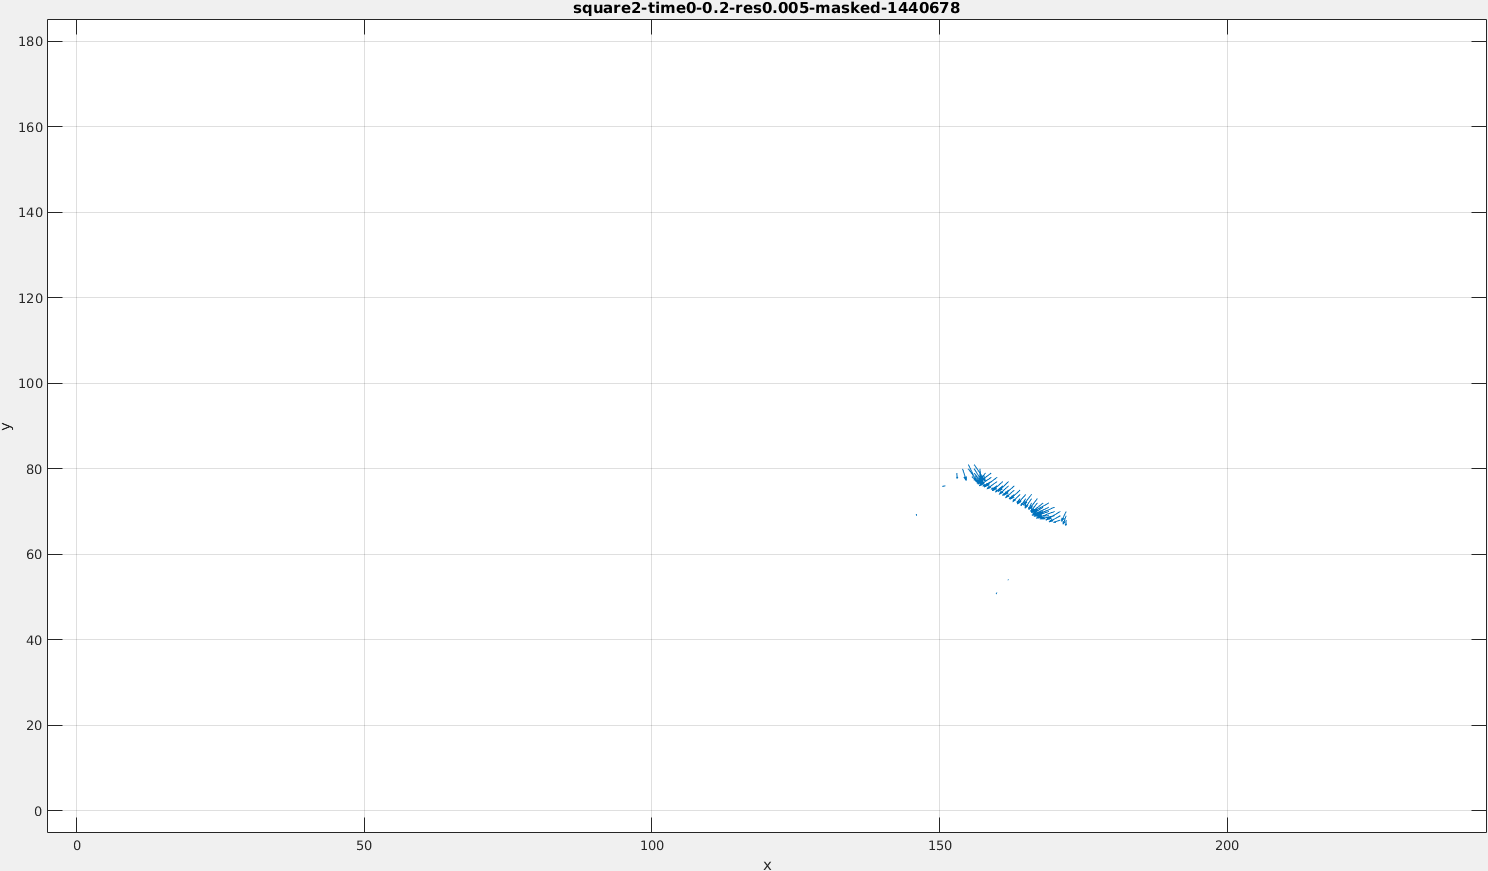
\includegraphics[height=.6\linewidth]{figs/square2/square2-masked-1.png}
  \caption{}
\end{subfigure}
\begin{subfigure}{.45\textwidth}
  \centering
  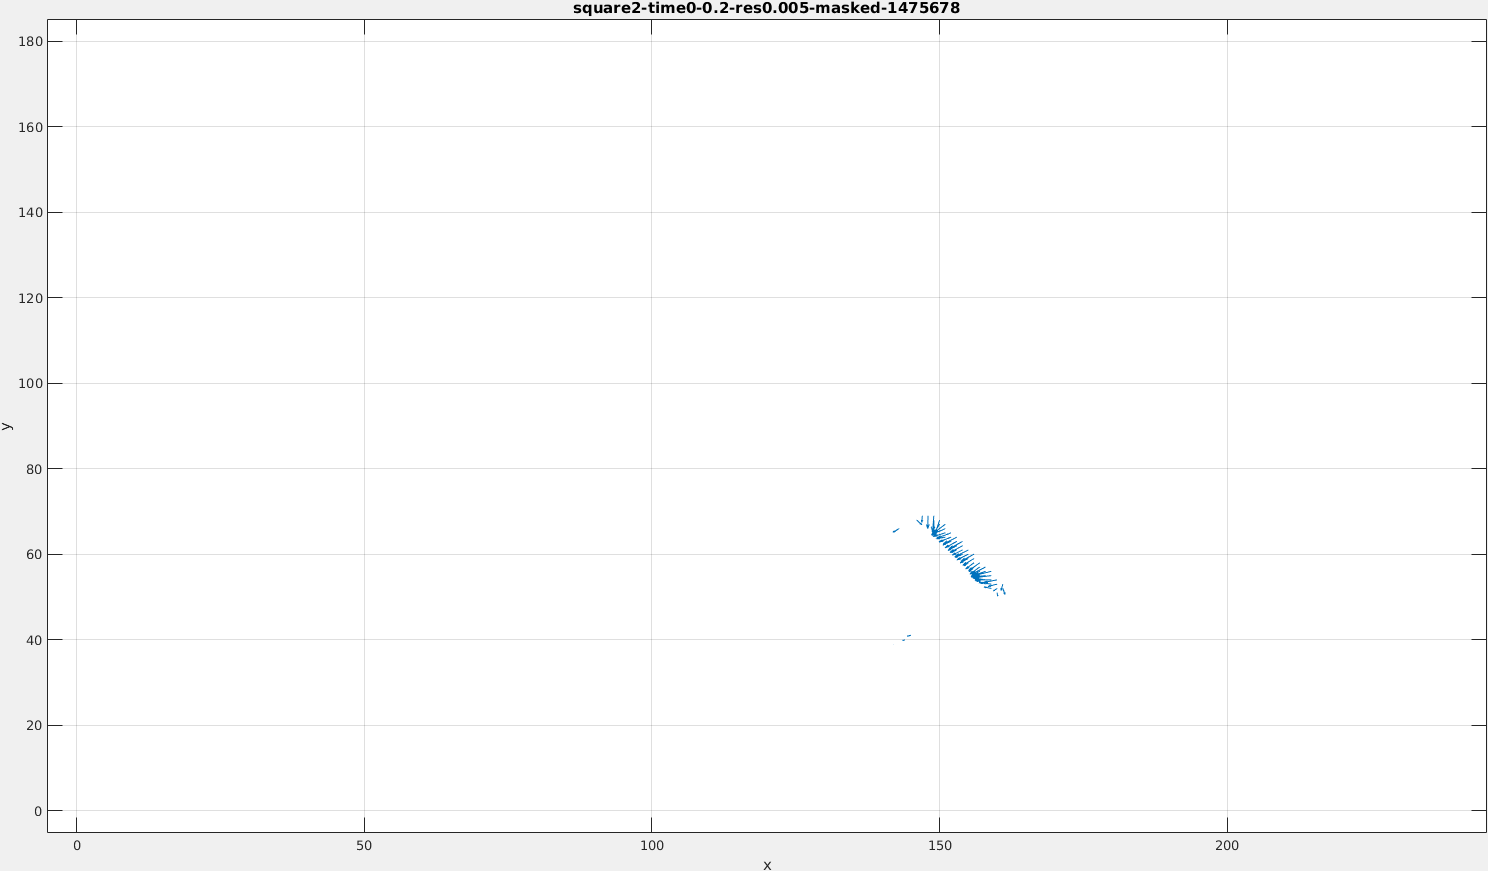
\includegraphics[height=.6\linewidth]{figs/square2/square2-masked-2.png}
  \caption{}
\end{subfigure}
\begin{subfigure}{.45\textwidth}
  \centering
  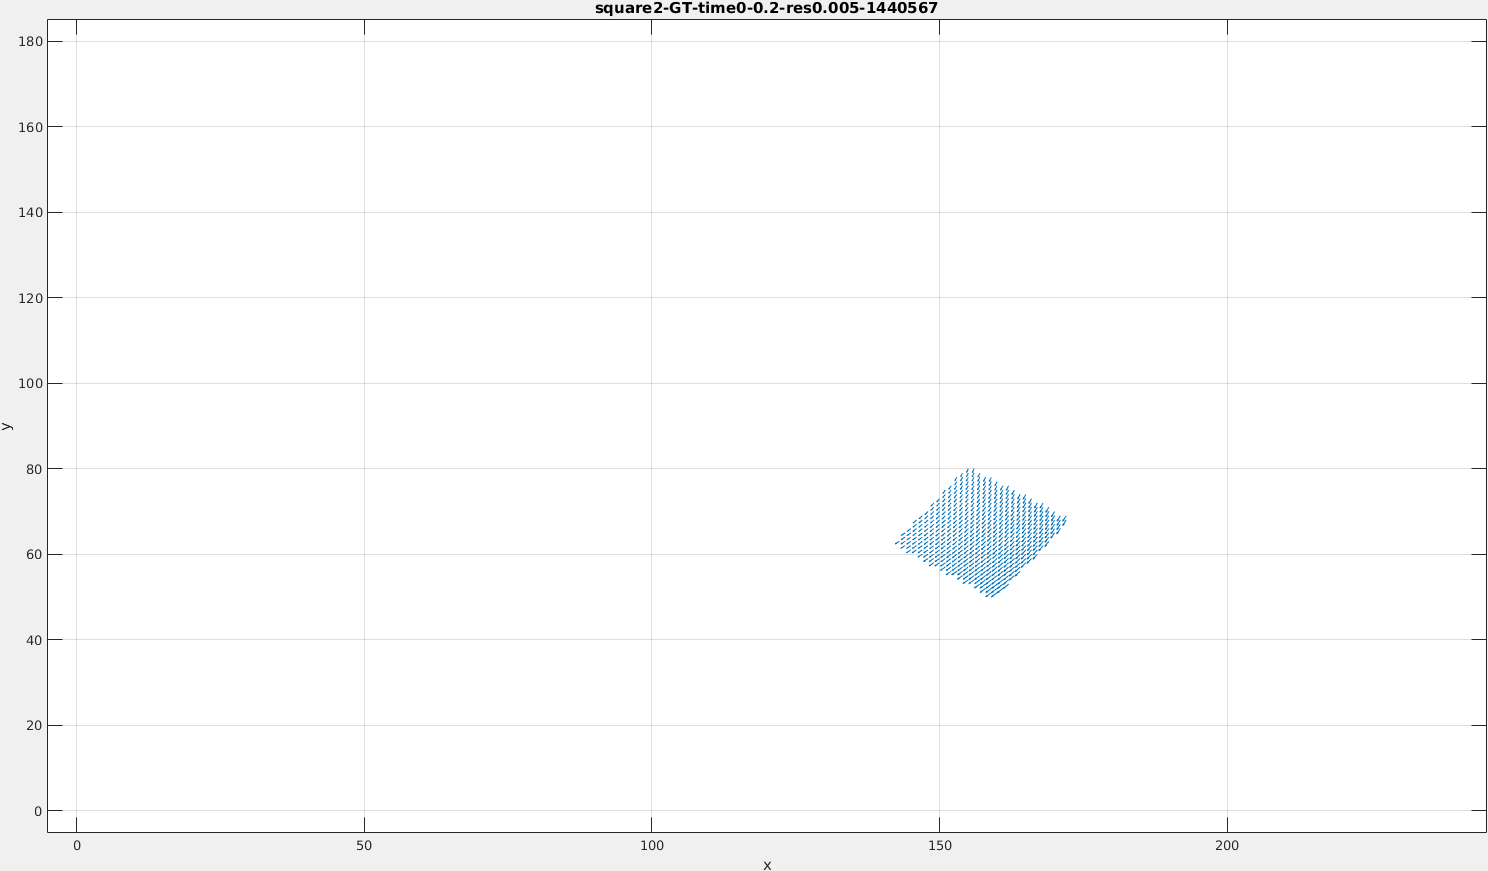
\includegraphics[height=.6\linewidth]{figs/square2/square2-GT-1.png}
  \caption{}
\end{subfigure}
\begin{subfigure}{.45\textwidth}
  \centering
  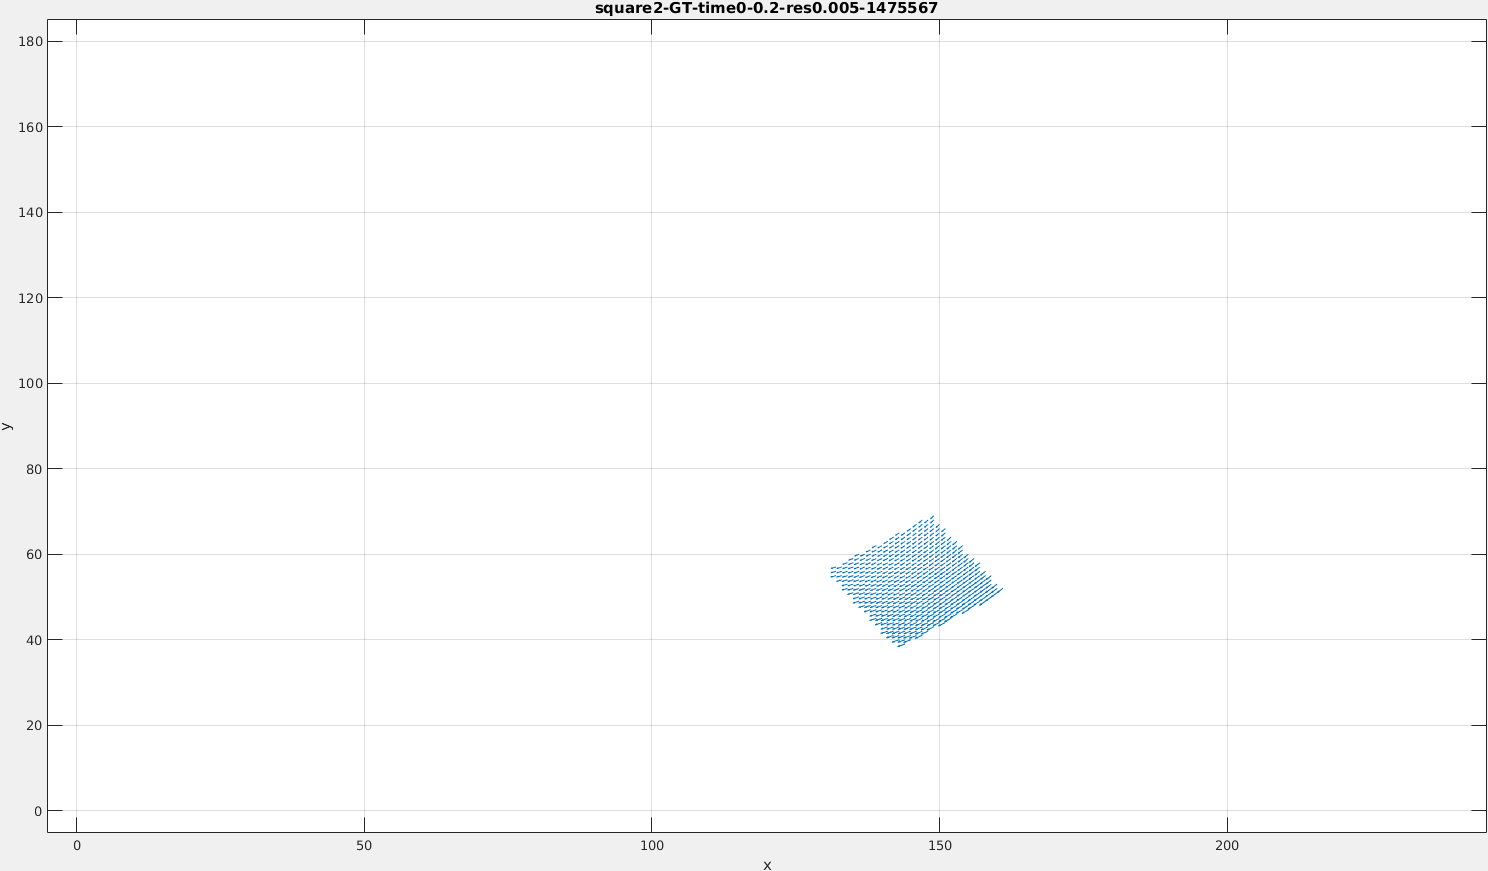
\includegraphics[height=.6\linewidth]{figs/square2/square2-GT-2.png}
  \caption{}
\end{subfigure}
\begin{subfigure}{.45\textwidth}
  \centering
  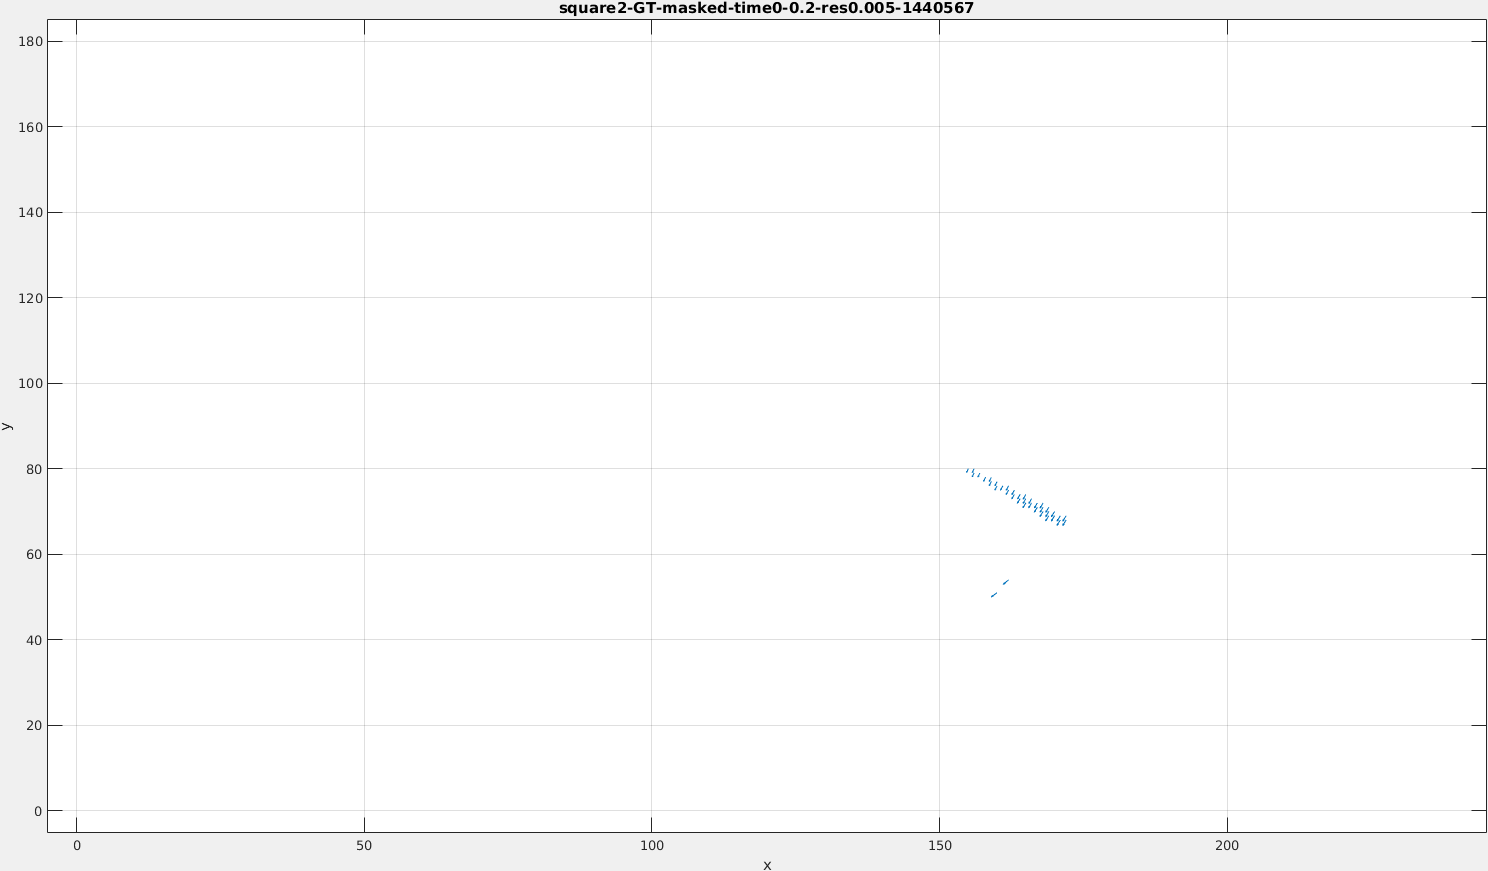
\includegraphics[height=.6\linewidth]{figs/square2/square2-GT-masked-1.png}
  \caption{}
\end{subfigure}
\begin{subfigure}{.45\textwidth}
  \centering
  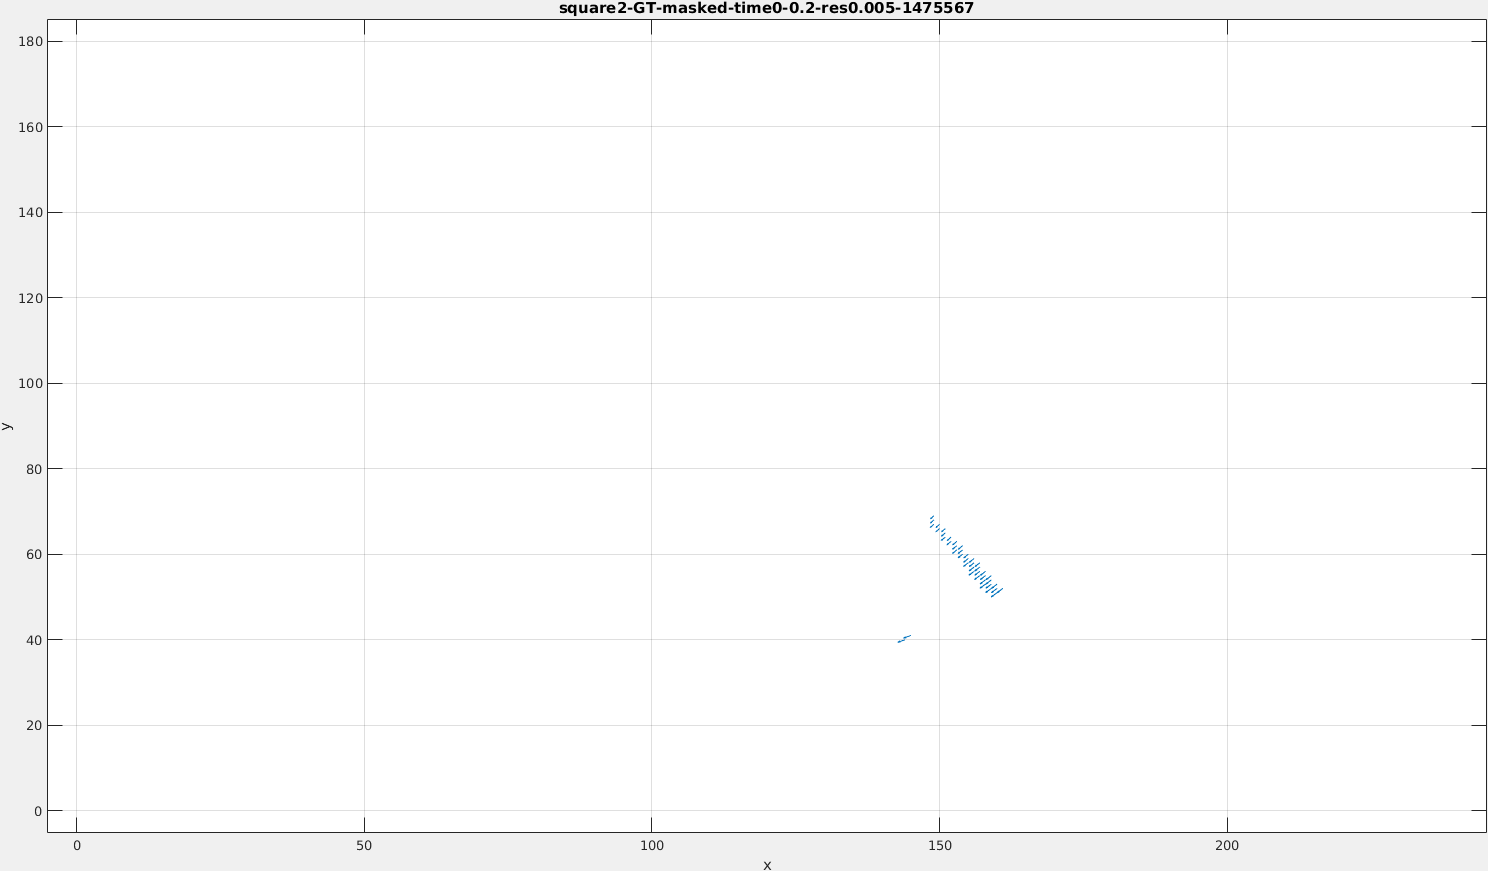
\includegraphics[height=.6\linewidth]{figs/square2/square2-GT-masked-2.png}
  \caption{}
\end{subfigure}
\caption[Fifth scene: Synthetic data of a circularly moving square.]{Fifth scene: Synthetic data of a circularly moving square.
Figures (a) and (b) show the computed optical flow for the scene at two time steps. The masked flow fields are shown in Figures (c) and (d).
The corresponding ground truth is shown in Figures (e) and (f). Applying the same mask leads to Figures (g) and (h)}
\label{fig:square2-snapshots}
\end{figure}


\begin{table}[tb]
	\centering
		\begin{tabular}{lccccccc}
Scene & Setting & Matching & RMSE & MeanErr & MedianErr & Avg. Angle \\
\hline  \hline
square2 & $13$ & direct & $32.57$ & $25.10$ & $19.81$ & -$150.44$ & \\
square2 & $13$ & interp & $32.92$ & $25.25$ & $19.79$ &  & \\
square2 & $14$ & direct & $32.77$ & $25.00$ & $19.31$ & -$150.63$ & \\
square2 & $14$ & interp & $33.19$ & $25.18$ & $19.30$ &  & \\
		\end{tabular}
	\caption[Fifth scene: Comparison of angular errors for different parameters.]{Fifth scene: Comparison of angular errors for different parameters.The angular error is rather low, considering the speed and non-linearity of the object's movement.
	A reason for this is the greatly reduced influenced effect of the missing normalization step.}
	\label{tab:error_comparison_square2}
\end{table}


The third synthetic scene depicts two balls moving around non-linear trajectories (see Figure \ref{fig:baelle-snapshots}). 
In Figures \ref{fig:baelle-snapshots1} and \ref{fig:baelle-snapshots2} it can be observed that the computed flow is influenced by the shading effect that was applied in the 3D scene. 

Due to the shading, the algorithm detects an additional edge inside one of the balls, which leads to more ambiguous results.
However, Table \ref{tab:error_comparison_baelle} shows that the median angular error is still rather low in comparison to other scenes.

A reason for this might be the shape of the balls. 
Without normalization, a part of the surface always roughly points in the movement direction, which leads to valid results for the corresponding event locations.

\begin{figure}[tb]
\centering
\begin{subfigure}{.45\textwidth}
  \centering
  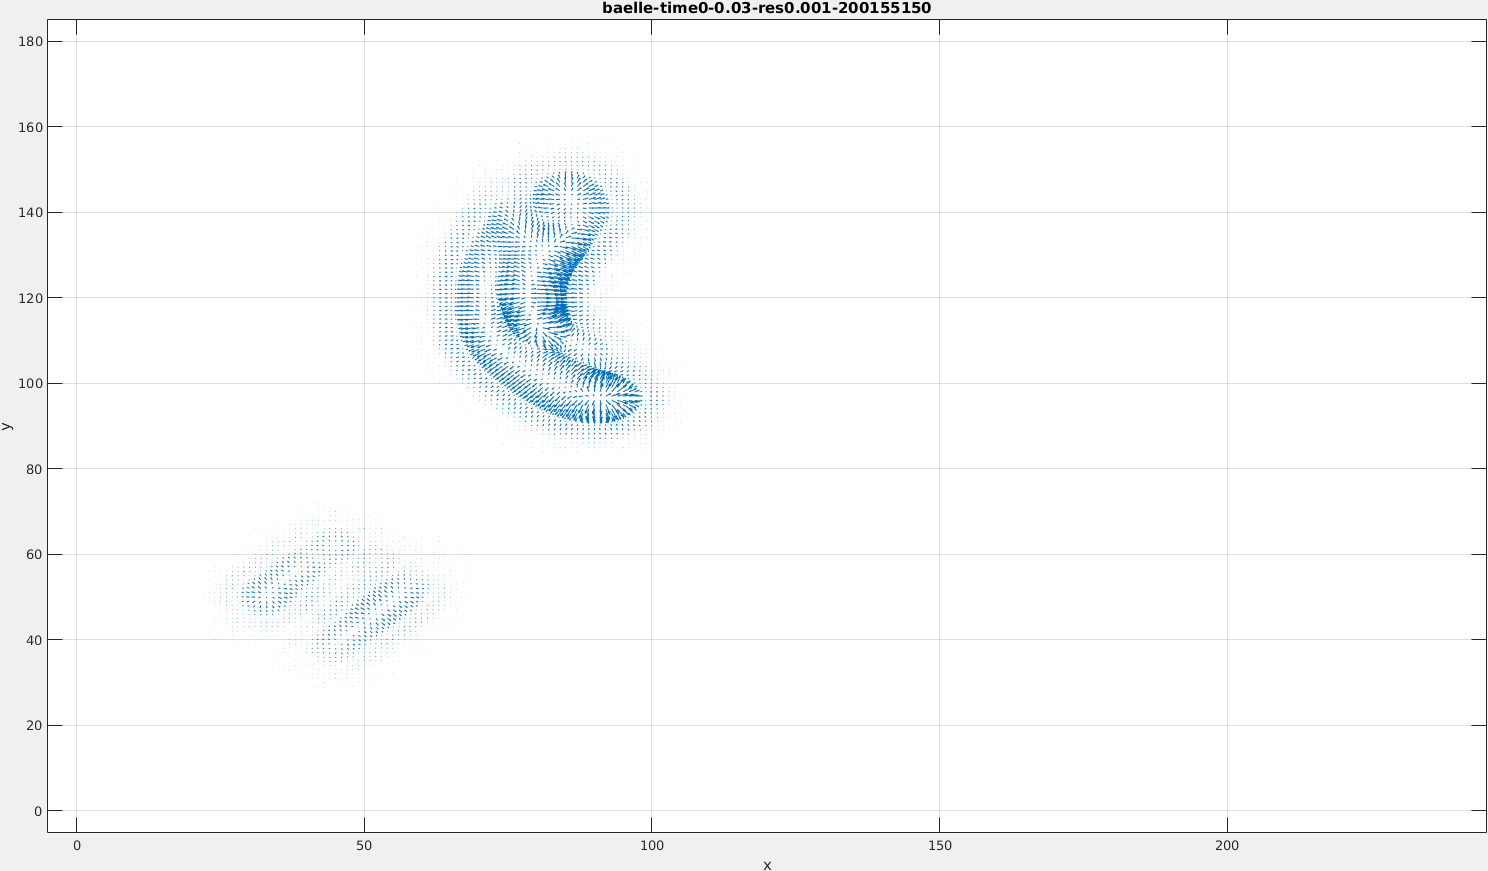
\includegraphics[height=.6\linewidth]{figs/baelle/baelle-1.png}
  \caption{}
\label{fig:baelle-snapshots1}
\end{subfigure}
\begin{subfigure}{.45\textwidth}
  \centering
  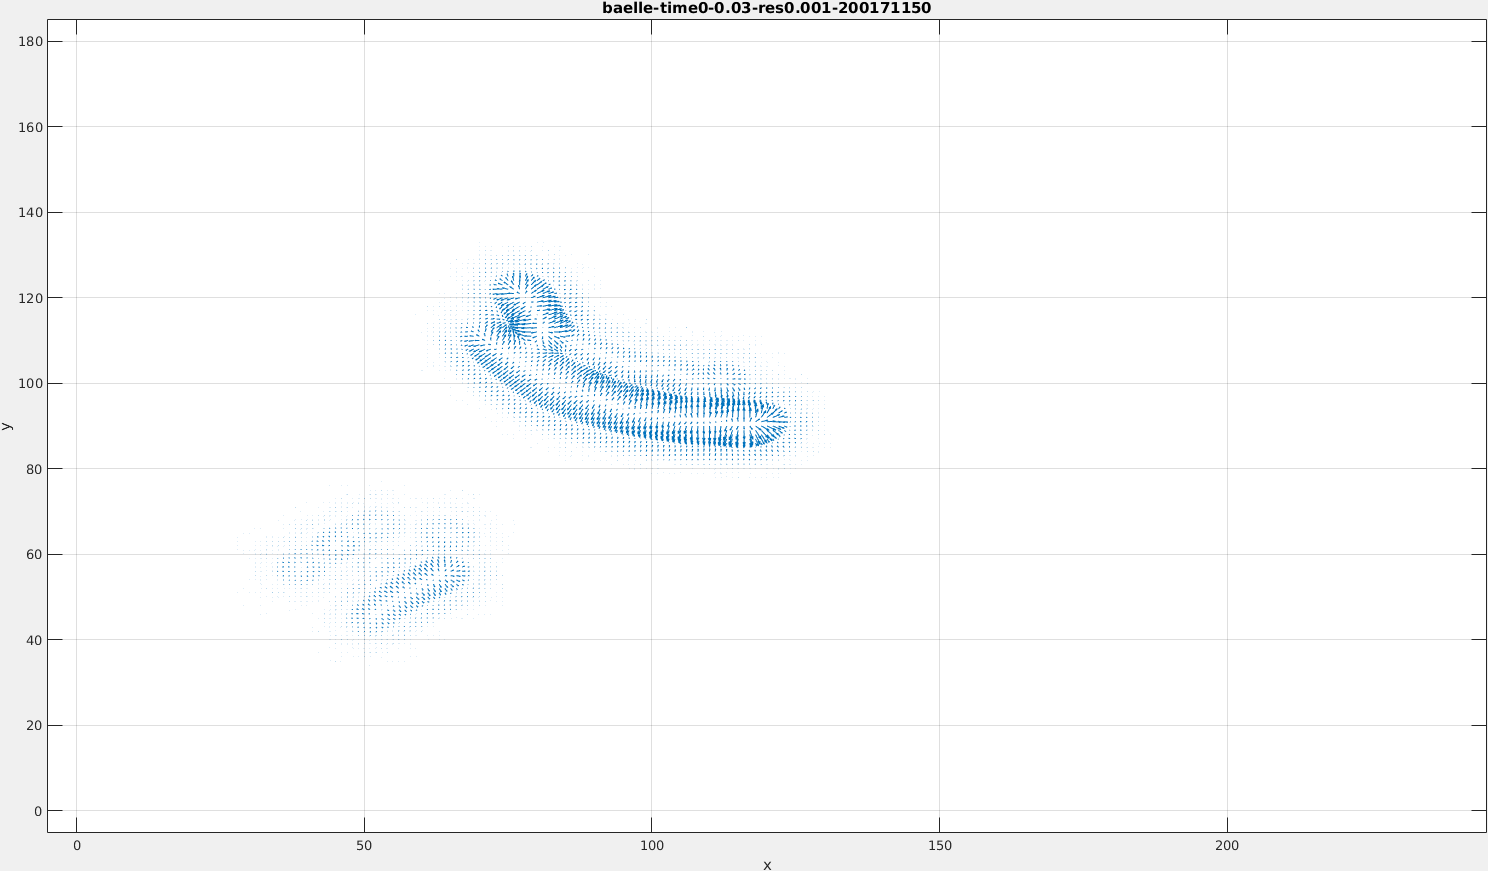
\includegraphics[height=.6\linewidth]{figs/baelle/baelle-2.png}
  \caption{}
  \label{fig:baelle-snapshots2}
\end{subfigure}
\begin{subfigure}{.45\textwidth}
  \includegraphics[height=.6\linewidth]{figs/baelle/baelle-masked-1.png}
  \caption{}
\end{subfigure}
\begin{subfigure}{.45\textwidth}
  \centering
  \includegraphics[height=.6\linewidth]{figs/baelle/baelle-masked-2.png}
  \caption{}
\end{subfigure}
\begin{subfigure}{.45\textwidth}
  \centering
  \includegraphics[height=.6\linewidth]{figs/baelle/baelle-GT-1.png}
  \caption{}
\end{subfigure}
\begin{subfigure}{.45\textwidth}
  \centering
  \includegraphics[height=.6\linewidth]{figs/baelle/baelle-GT-2.png}
  \caption{}
\end{subfigure}
\begin{subfigure}{.45\textwidth}
  \centering
  \includegraphics[height=.6\linewidth]{figs/baelle/baelle-GT-masked-1.png}
  \caption{}
\end{subfigure}
\begin{subfigure}{.45\textwidth}
  \centering
  \includegraphics[height=.6\linewidth]{figs/baelle/baelle-GT-masked-2.png}
  \caption{}
\end{subfigure}
\caption[Sixth scene: Synthetic data of two balls moving through the scene.]{Sixth scene: Synthetic data of two balls moving through the scene.
Figures (a) and (b) show the computed optical flow for the scene at two time steps. The masked flow fields are shown in Figures (c) and (d).
The corresponding ground truth is shown in Figures (e) and (f). Applying the same mask leads to Figures (g) and (h).
Due to a shading effect, two edges are detected by the algorithm (a)(b).}
\label{fig:baelle-snapshots}
\end{figure}

\begin{table}[tb]
	\centering
		\begin{tabular}{lccccccc}
Scene & Setting & Matching & RMSE & MeanErr & MedianErr & Avg. Angle \\
\hline  \hline
baelle & $15$ & direct & $43.46$ & $33.57$ & $26.39$ & $13.11$ & \\
baelle & $15$ & interp & $43.44$ & $33.48$ & $26.10$ &  & \\
baelle & $16$ & direct & $42.88$ & $33.38$ & $26.61$ & $13.41$ & \\
baelle & $16$ & interp & $42.81$ & $33.26$ & $26.37$ &  & \\
		\end{tabular}
	\caption[Sixth scene: Comparison of angular errors for different parameters.]{Sixth scene: Comparison of angular errors for different parameters.
	The median angular error is rather low compared to other investigated scenes. 
	This could be caused by the reduced effect of missing normalization due to the circular shape of the objects.}
	\label{tab:error_comparison_baelle}
\end{table}


Overall, the results of the evaluation seem promising.
A major part of the angular errors can be accounted for by the missing normalization in the post-processing.
Furthermore, the filter bank only incorporated Gabor filters with a fixed speed selectivity.
The problem of simultaneous movement of all pixels of an edge did only occur in the synthetic data and is unlikely to happen in real scenarios.
Nevertheless it should be addressed in further investigations.
